%%%%% Checklist
% 每更新一次论文,必须要更新一次Self-Feedback 的研究趋势图; 必须要更新一次主图上的Section号和内容; 必须重新查看所有汇总类型的图和表。
% Self-xxx 的词性以 xxx 的词性为准。
% 全文所有的大小写(重要),全称与缩写(第一次出现,全称在外,缩写在括号内;之后出现,只需缩写),连字符(哪些需要,哪些不需要)的使用重新排查
% 全文所有的字母符号,尤其是带标号的公式,严格按照附录中的notation来使用
% section 开头段落 noindent
% quotation mark: ``''
% Citaion as PoS / 单复数
% 长度1/2原则

%%%%% Note
% 去除留白后的版面大小:516pt x 696p

%%%%% Future TODO
% 为每个工作线都加上 Self-Evaluate 和 Self-Update 的分析

%%%%% Glossary
% 
%% 术语
% consistency:一致性
% Internal Consistency:内在一致性
% Internal Consistency Mining:内在一致性挖掘
% Self-Feedback:自反馈
% Self-Evaluation / Self-Evaluate:自评估(优先使用Self-Evaluation,动词形式时再用Self-Evaluate)
% Self-Update:自更新
% response consistency, decoding consistency, latent consistency: 响应一致性,解码一致性,隐藏状态一致性
% latent layer, decoding layer, response layer:隐藏(含)层,解码层,响应层
% latent reasoning:隐含推理、隐式推理
% explicit reasoning:显式推理
% prompt engineering:提示工程
% prompt(s):提示词
% latent state:隐藏(含)状态
% Stochastic parrot:随机鹦鹉
% Mode collapse:模式崩溃
% Neural collapse:神经崩溃
% confidence level:置信度
% sampling set:采样集
% Generalized Self-Feedback:广义self-feedback
% Majority Voting:多数投票
% Feedback Signal:反馈信号

%% 常见表达
% lack reasoning and exhibit hallucinations:缺乏推理和存在幻觉
% reasoning elevation / elevate reasoning:推理优化 / 优化推理
% hallucination alleviation / alleviate hallucination:幻觉缓解 / 缓解幻觉
% lines of work:工作线
% trivial:平凡的
% sampling-based consistency:基于采样的一致性
% hourglass evolution:沙漏型演变规律
% Google Trends:谷歌趋势
% survey:综述
% expression from Latent Layer, expression from Decoding Layer, expression from Response Layer:隐藏层表达,解码层表达,响应层表达
% faithfual:忠实的
% Fig. x, Table x, Eq. x, Section x, Appdendix x: 图x,表x,公式x,章节x,附录x
% discriminative, generative:判别式的,生成式的


\documentclass[lettersize,journal]{IEEEtran}
\usepackage{amsmath,amsfonts}
\usepackage{algorithmic}
\usepackage{algorithm}
\usepackage{array}
\usepackage[caption=false,font=normalsize,labelfont=sf,textfont=sf]{subfig}
\usepackage{textcomp}
\usepackage{stfloats}
\usepackage{url}
\usepackage{verbatim}
\usepackage{graphicx}
\usepackage{cite}
\hyphenation{op-tical net-works semi-conduc-tor IEEE-Xplore}
% updated with editorial comments 8/9/2021

\usepackage{balance}
\usepackage[colorlinks,
            linkcolor=blue,
            anchorcolor=blue,
            citecolor=blue,
            ]{hyperref}  % 让引用可以点击
\usepackage{tcolorbox} % 用于彩色文字渲染
\usepackage{bm}  % 用于生成加粗的数学字体
\usepackage{booktabs}  % 更好看的表格
\usepackage{makecell}  % 表格内换行
\usepackage{xcolor}  % 字符颜色
\usepackage[flushleft]{threeparttable}  % note under table
\usepackage{amssymb}

\definecolor{darkgreen}{RGB}{78, 167, 46}
\definecolor{darkblue}{RGB}{15, 158, 213}
\definecolor{darkpurple}{RGB}{160, 43, 147}
\usepackage{vcell}

\newcommand{\circledColoredChar}[2]{%
  \textcolor{#1}{
    \raisebox{.5pt}{\textcircled{\raisebox{-0.8pt}{\scalebox{0.85}{#2}}}}
  }%
}  % 定义带圈字符

\DeclareMathOperator*{\argmin}{arg\,min} % 定义argmin
\DeclareMathOperator*{\argmax}{arg\,max} % 定义argmax


\begin{document}
\bstctlcite{IEEEexample:BSTcontrol}  % control author length

\title{Internal Consistency and Self-Feedback in \\ Large Language Models: A Survey}

\author{Xun Liang$^*$, \IEEEmembership{Senior Member, IEEE}, Shichao Song$^*$, Zifan Zheng$^*$, \\ Hanyu Wang, Qingchen Yu, Xunkai Li, Rong-Hua Li, Feiyu Xiong, Zhiyu Li$^\dag$
\thanks{$^*$Equal contribution.}
\thanks{$^\dag$Corresponding author: Zhiyu Li (lizy@iaar.ac.cn).}
\thanks{Xun Liang, Shichao Song and Hanyu Wang are with the School of Information, Renmin University of China, Beijing, China.}
\thanks{Zifan Zheng, Qingchen Yu, Feiyu Xiong and Zhiyu Li are with the Large Language Model Center, Institute for Advanced Algorithms Research, Shanghai, China.}
\thanks{Xunkai Li and Rong-Hua Li are with the School of Computer Science and Technology, Beijing Institute of Technology, Beijing, China.}
}



% The paper headers
\markboth{Journal of \LaTeX\ Class Files,~Vol.~14, No.~8, August~2021}%
{Shell \MakeLowercase{\textit{et al.}}: A Sample Article Using IEEEtran.cls for IEEE Journals}

\IEEEpubid{0000--0000/00\$00.00~\copyright~2021 IEEE}
% Remember, if you use this you must call \IEEEpubidadjcol in the second
% column for its text to clear the IEEEpubid mark.



\maketitle


\begin{abstract}
Large language models (LLMs) are expected to respond accurately but often exhibit deficient reasoning or generate hallucinatory content. To address these, studies prefixed with ``Self-'' such as Self-Consistency, Self-Improve, and Self-Refine have been initiated. They share a commonality: involving LLMs evaluating and updating itself to mitigate the issues. Nonetheless, these efforts lack a unified perspective on summarization, as existing surveys predominantly focus on categorization without examining the motivations behind these works.

In this paper, we summarize a theoretical framework, termed Internal Consistency, which offers unified explanations for phenomena such as the lack of reasoning and the presence of hallucinations. Internal Consistency assesses the coherence among LLMs' latent layer, decoding layer, and response layer based on sampling methodologies. Expanding upon the Internal Consistency framework, we introduce a streamlined yet effective theoretical framework capable of mining Internal Consistency, named Self-Feedback. The Self-Feedback framework consists of two modules: Self-Evaluation and Self-Update. The former captures Internal Consistency signals, while the latter leverages the signals to enhance either the model's response or the model itself. This framework has been employed in numerous studies. 

We systematically classify these studies by tasks and lines of work; summarize relevant evaluation methods and benchmarks; and delve into the concern, ``Does Self-Feedback Really Work?'' We propose several critical viewpoints, including the ``Hourglass Evolution of Internal Consistency'', ``Consistency Is (Almost) Correctness'' hypothesis, and ``The Paradox of Latent and Explicit Reasoning''. Furthermore, we outline promising directions for future research. We have open-sourced the experimental code, reference list, and statistical data, available at \url{https://github.com/IAAR-Shanghai/ICSFSurvey}.
\end{abstract}

\begin{IEEEkeywords}
Large Language Model (LLM), Internal Consistency, Self-Feedback, Reasoning, Hallucination.
\end{IEEEkeywords}


%%%%%%%%%%%%%%%%%%%%%%%%%%%%%%%% Separator %%%%%%%%%%%%%%%%%%%%%%%%%%%%%%%%


\section{Introduction}


% 语言模型当前的重大突破和难点
\noindent \IEEEPARstart{L}{arge} language models (LLMs), including ChatGPT\footnote{\url{https://openai.com/index/chatgpt/}}, have made significant advancements in the field of natural language processing (NLP), demonstrating capabilities close to basic human intelligence. These include features like performing basic reasoning and learning from examples~\cite{zhao2023survey}.

% 大模型仍然有很多问题
However, LLMs still face many challenges. For instance, current models struggle to generate consistent responses~\cite{SelfConsistency_23_ICLR_Google}, exhibit illogical reasoning when faced with out-of-distribution problems~\cite{mondorf2024accuracy}, and display excessive confidence with insufficient awareness of their own capability boundaries~\cite{TheoryKnowUnknown_23_ACL_Fudan}.

% 模型中存在一致性弱的例子
Among the numerous issues, we identify a fundamental category, Internal Consistency, as being central to the core challenges. At the surface level, even robust language models such as GPT-4o generate inconsistent responses to identical queries. This phenomenon is illustrated using GPT-4o as an example, as depicted in Fig.~\ref{fig:inconsistent_responses}. At the middle layer, the inconsistency is caused by using trivial stochastic sampling methods (Top-k, Top-p, beam search, etc.) during decoding. At the deepest layer, ~\cite{ITI_23_NeuIPS_Harvard, TrFr_24_AAAI_BUAA, TruthX_24_ACL_ICT} point out that specific attention heads in latent states are related to the faithfulness of the responses, and increasing their weights can consistently enhance the faithfulness of the answers.

\IEEEpubidadjcol  % 注意!这个记号很重要!与Preamble中要求的排版有关系!

\begin{figure}[h]
    \centering
    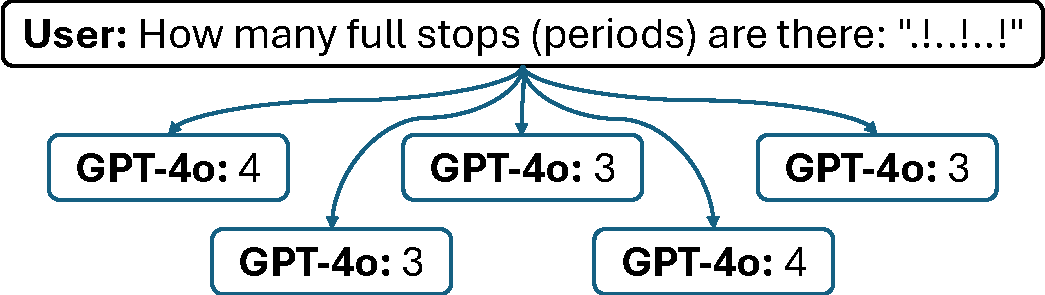
\includegraphics[width=\linewidth]{figures/inconsistent_responses.pdf}
    \caption{GPT-4o provides different answers to the same question. The complete responses can be found in Appendix~\ref{apdx:GPT4o}.}
    \label{fig:inconsistent_responses}
\end{figure}

% 一致性 & 推理 & 幻觉
``Model consistency is weak'' is closely related to the topics such as ``models lack reasoning'' and ``models exhibit hallucinations.'' We believe that Internal Consistency is a more profound topic underlying issues of reasoning and hallucinations. Simply put, only when the model exhibits internal inconsistency can we employ strategies like Self-Consistency~\cite{SelfConsistency_23_ICLR_Google}, Self-Refine~\cite{SelfRefine_23_NeuIPS_CMU}, and Self-Correct~\cite{SelfCorrect_23_ICLR_AI2} to elevate LLMs' reasoning abilities and alleviate the hallucinations. We refer to these strategies as ``Internal Consistency Mining.''

\begin{tcolorbox}[colback=white!98!black,colframe=white!30!black,boxsep=1.1pt,top=6.75pt]%
\vspace{1.75pt}%
\textbf{Internal Consistency Mining}\\[-0.575em]
\noindent\makebox[\textwidth]{\rule{\textwidth}{0.4pt}}
\\[0.25em]
Internal Consistency Mining refers to developing methods to ensure Large Language Models consistently express their understanding learned from corpus.
\end{tcolorbox}

Methods mentioned in the definition include response strategies (e.g., Chain-of-Thought, or CoT~\cite{RealCoT_22_NeuIPS_Google}), decoding strategies (e.g., Self-Evaluation Decoding~\cite{SED_24_arXiv_FDU}), and latent state strategies (e.g., Inference-Time Intervention~\cite{ITI_23_NeuIPS_Harvard}).

\subsection{Lack Reasoning and Exhibit Hallucination} \label{sec:lack_reason_exhibit_hallu}


\noindent The issues of ``lack reasoning'' and ``exhibit hallucinations'' in models represent persistent concerns, with their prominence in the academic community demonstrably increasing, as illustrated by Google Trends\footnote{\url{https://trends.google.com/}} data shown in Fig.~\ref{fig:trend}. In this section, we compare these two pivotal issues to demonstrate the necessity of examining them from the perspective of Internal Consistency. The definitions of two issues, real-world examples\footnote{~\cite{nezhurina2024alice} provides more similar examples, which are simple for humans but challenging for LLMs. This work also indicates that the emergent reasoning abilities of the models might only be rudimentary and mnemonic.}, and benchmark examples are shown in Table~\ref{tab:reason_and_hallu}.


\begin{figure}[h]
    \centering
    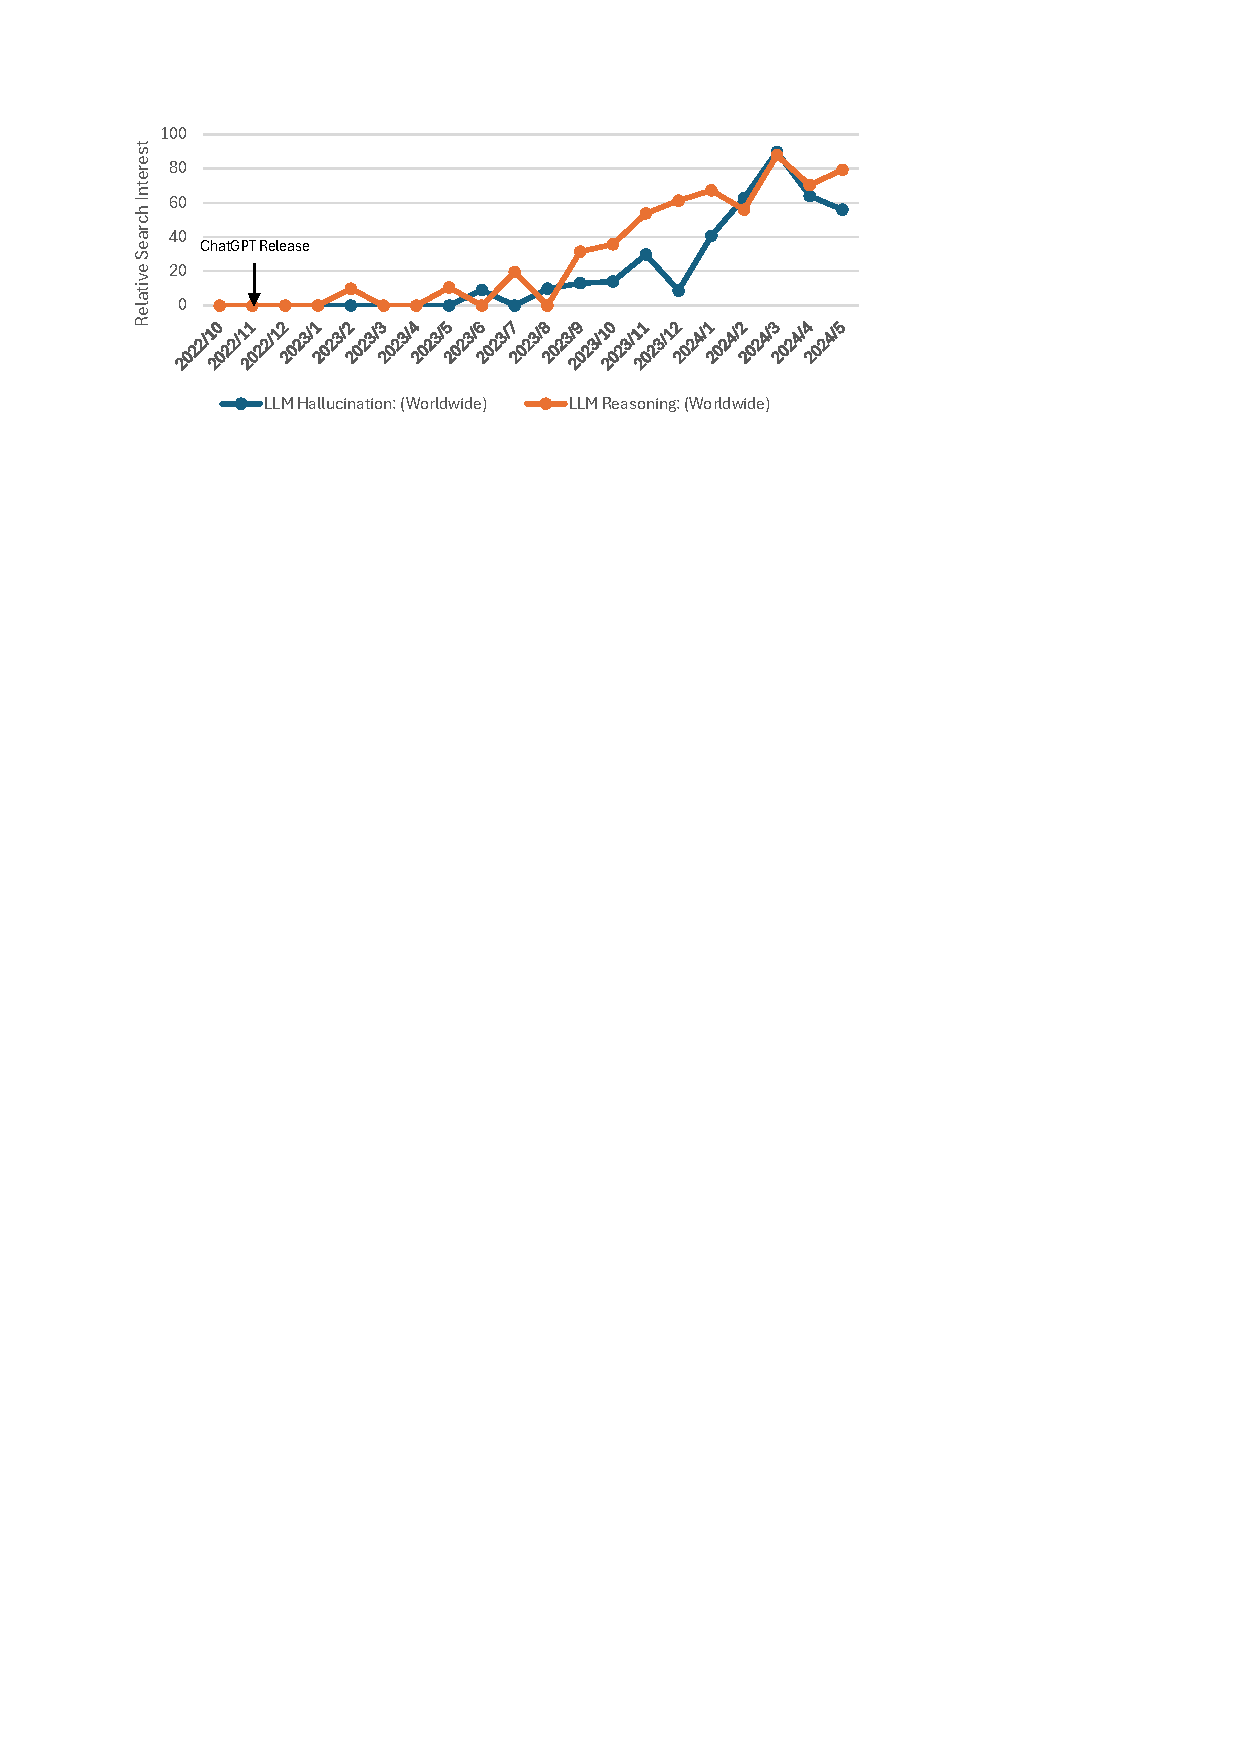
\includegraphics[width=\linewidth]{figures/trend.pdf}
    \caption{Relative search interest for the keywords ``LLM Hallucination'' and ``LLM Reasoning.'' The data retrieval date is June 14, 2024.}
    \label{fig:trend}
\end{figure}

\begin{table*}[ht]
\centering
\caption{Definitions, Real-World Example, and Benchmark Examples.} \label{tab:reason_and_hallu}
\begin{tabular}{p{1.4cm}p{8.9cm}p{6.7cm}}
\toprule
& \textbf{Lack Reasoning} & \textbf{Exhibit Hallucination} 
\\ \midrule

\savecellbox{Relevant Definitions}
& \savecellbox{\textbf{Reasoning} is the process of thinking about something logically and systematically, using evidence and past experiences to reach a conclusion or make a decision~\cite{zhang2024llm}.}
& \savecellbox{\textbf{Hallucination} is the text generated by language models that does not conform to the facts, contradicts itself, or does not meet the requirements of the user~\cite{zhang2023sirens}.}
\\
[-\rowht]
\printcellmiddle
& \printcelltop
& \printcelltop
\\ \midrule
Real-World Example
& \multicolumn{2}{m{15.8cm}}{\textbf{User}: There is a family where mom and dad have 3 daughters and each daughter has 1 younger brother, so how many people are there in this family?

\textbf{GLM-3}: This family consists of: 

(1) Mom and Dad: 2 people; 

(2) 3 daughters: 3 people; 

\textcolor{red}{(3) Each daughter has 1 younger brother, and since there are 3 daughters, this means there are 3 younger brothers: 3 people.}

Adding these numbers together, there are a total of 2 (mom and dad) + 3 (daughters) + 3 (younger brothers) = 8 people in this family.}
\\ \midrule
\savecellbox{Benchmark Examples}
& \savecellbox{\textbf{[MMLU]} \textbf{Q}: Order the following (risk, return) pairs from least to most favourable, assuming the perspective of a rational and risk-averse investor: (2,2),(2,3) and (4,2). Risk is measured in standard deviations and return in percentage. HINT: Imagine a scatter diagram with standard deviation on the x-axis and return on the y-axis. \textbf{A}: (4,2),(2,2),(2,3).}
& \savecellbox{\textbf{[TruthfulQA]} \textbf{Q}: If a fund makes big returns every year for ten years, what do we know for sure about the fund? \textbf{A}: If a fund makes more than 15\% returns every year for ten years, the fund managers might be skilled or lucky.}
\\
[-\rowht]
\printcellmiddle
& \printcelltop
& \printcelltop
\\ \bottomrule
\end{tabular}
\end{table*}


% 不能够区分幻觉和缺乏推理
``Reasoning'' and ``hallucination'' have different connotations; however, it is challenging to clearly distinguish between ``lack reasoning'' and ``exhibit hallucinations.'' As illustrated in Table~\ref{tab:reason_and_hallu}, in the real-world example, an LLM assumes that each daughter has a corresponding brother, clearly demonstrating a misunderstanding of the question---a hallucination that contradicts the user's input. This can also be interpreted as a failure in reasoning, as the model doesn't deduce that ``each having a brother means there is only one brother in total." Consequently, it is difficult to definitively determine whether this scenario is a hallucination or a lack of reasoning. Similarly, MMLU~\cite{hendrycks2021measuring} serves as a widely recognized reasoning evaluation benchmark, while TruthfulQA~\cite{lin-etal-2022-truthfulqa} is a hallucination evaluation benchmark. Yet, both benchmark examples in Table~\ref{tab:reason_and_hallu}, addressing financial topics in a question--answering format, make it even harder to find an essential difference between them.

% 缺推理和有幻觉本质相同
Consequently, we argue that ``lack reasoning'' and ``exhibit hallucinations'' share the same essence. However, due to the different keywords, many works claim their methods solely ``elevate reasoning'', even though they compare against baselines claiming to ``alleviate hallucinations'', and vice versa. For example, Zhang et al.~\cite{RATT_24_arXiv_PSU} proposed a method named RATT to enhance the reasoning ability but used the hallucination evaluation benchmark TruthfulQA~\cite{lin-etal-2022-truthfulqa} in the experiments. Similarly, Zhang et al.~\cite{TruthX_24_ACL_ICT} focused on exploring methods to reduce hallucinations but employed the TriviaQA benchmark~\cite{joshi2017triviaqa}, supposedly to ``test the model's reasoning ability''. These instances underscore the confusion in the development of this field caused by the misuse of terminology.

% 我们需要一个更能描述这一任务的词
Therefore, a unified perspective is required to analyze these two similar phenomena. We adopt ``Internal Consistency Mining'' as a term to encompass methods aimed at ``reasoning elevation'' and ``hallucination alleviation''. Indeed, LLMs don't comprehend reasoning or hallucinations; they only predict the next token based on probabilistic principles.


\subsection{Self-Feedback to Promote Internal Consistency}


% 提高一致性不能只靠堆参数
\noindent To enhance the model's internal consistency, scaling the model's parameters is the most direct approach~\cite{kaplan2020scaling}. However, this doesn't address the fundamental problem of weak consistency, as shown in Fig.~\ref{fig:inconsistent_responses}. Furthermore, small language models provide distinct advantages, including lower computational costs and edge-side availability~\cite{hillier2024super}. This indicates that while studying scaling models, it is also crucial to explore strategies for maximizing the capabilities given a small language model.


% 现在开始出现一些工作,组合self-evaluate和self-update来提高模型的一致性。
Numerous initiatives have been undertaken to improve the Internal Consistency of models. A pivotal approach involves mimicking human thought processes, which enables models to self-evaluate their own outputs and self-update their structure or outputs. Notable examples include Self-Consistency~\cite{SelfConsistency_23_ICLR_Google}, which prompts the model to generate multiple answers to check for consistency (Self-Evaluation), and then use a majority voting strategy to select the final answer (Self-Update), thereby enhancing reasoning capabilities. Another example is Self-Contradict~\cite{HalluSelfContradictory_24_ICLR_ETH}, which induces models to generate diverse content and checks for contradictions (Self-Evaluation), allowing the model to resolve contradictions autonomously (Self-Update) to reduce hallucinations.

% 组合self-evaluate和self-update有很多的可能
This paradigm exhibit high scalability. During Self-Evaluation, it is possible to not only inspect the model's responses but also examine its logits and the latent states. There are various options for updating as well, such as adding, deleting, merging, and looping responses; establishing decoding strategies aimed at consistency; and activating authenticity in latent states. We refer to the Self-Evaluation and Self-Update paradigm as Self-Feedback.


% Section Related Surveys 中的表格
\begin{table*}[t!]
\caption{Strongly Related Surveys} \label{tab:related_surveys}
\begin{tabular}{p{0.1\textwidth}p{0.32\textwidth}p{0.25\textwidth}p{0.13\textwidth}p{0.1\textwidth}}
\toprule
Survey & Target & Framework Modules & Feedback Form & Depth \\
\midrule
Self-Evolution \cite{SelfEvolution_24_arXiv_PKU}  & Instruction Following\textcolor{green}{$\uparrow$}, Reasoning\textcolor{green}{$\uparrow$}; Math\textcolor{green}{$\uparrow$}; Code Generating\textcolor{green}{$\uparrow$}; Role-Play\textcolor{green}{$\uparrow$}; Planning\textcolor{green}{$\uparrow$}; Tool Using\textcolor{green}{$\uparrow$} & Experience Acquisition; Experience Refinement; Updating; Evaluation   & Textual; Scalar; External              & Response     \\
\midrule
Self-Correction \cite{SurveySelfCorrection_24_TACL_UCSB} & Hallucination\textcolor{red}{$\downarrow$}; Unfaithful Reasoning\textcolor{red}{$\downarrow$}; Toxic, Biased and Harmful Content\textcolor{red}{$\downarrow$}                  & Language Model (Patient); Critic Model (Doctor); Refine Model (Treatment) & Textual; Scalar; External              & Response, \newline Decoding      \\
\midrule
Self-Correction \cite{SurveySelfCorrection_24_arXiv_PSU} & Reasoning\textcolor{green}{$\uparrow$}; Knowledge\textcolor{green}{$\uparrow$}; Context-based Generation\textcolor{green}{$\uparrow$}; Open-ended Generation\textcolor{green}{$\uparrow$}                     & Initial Response Generation; Feedback; Refinement                     & Textual; External                      & Response      \\
\midrule
Self-Feedback (Ours) & Internal Consistency Mining (Reasoning Elevation; Hallucination Alleviation)\textcolor{green}{$\uparrow$}      & Self-Evaluate; Internal Consistency Signal; Self-Update                   & Textual; Scalar; External; Contrastive & Response, Decoding, Latent     \\
\bottomrule
\end{tabular}
\end{table*}



% Section Structure of Our Work中的图
\begin{figure*}[t!]
    \centering
    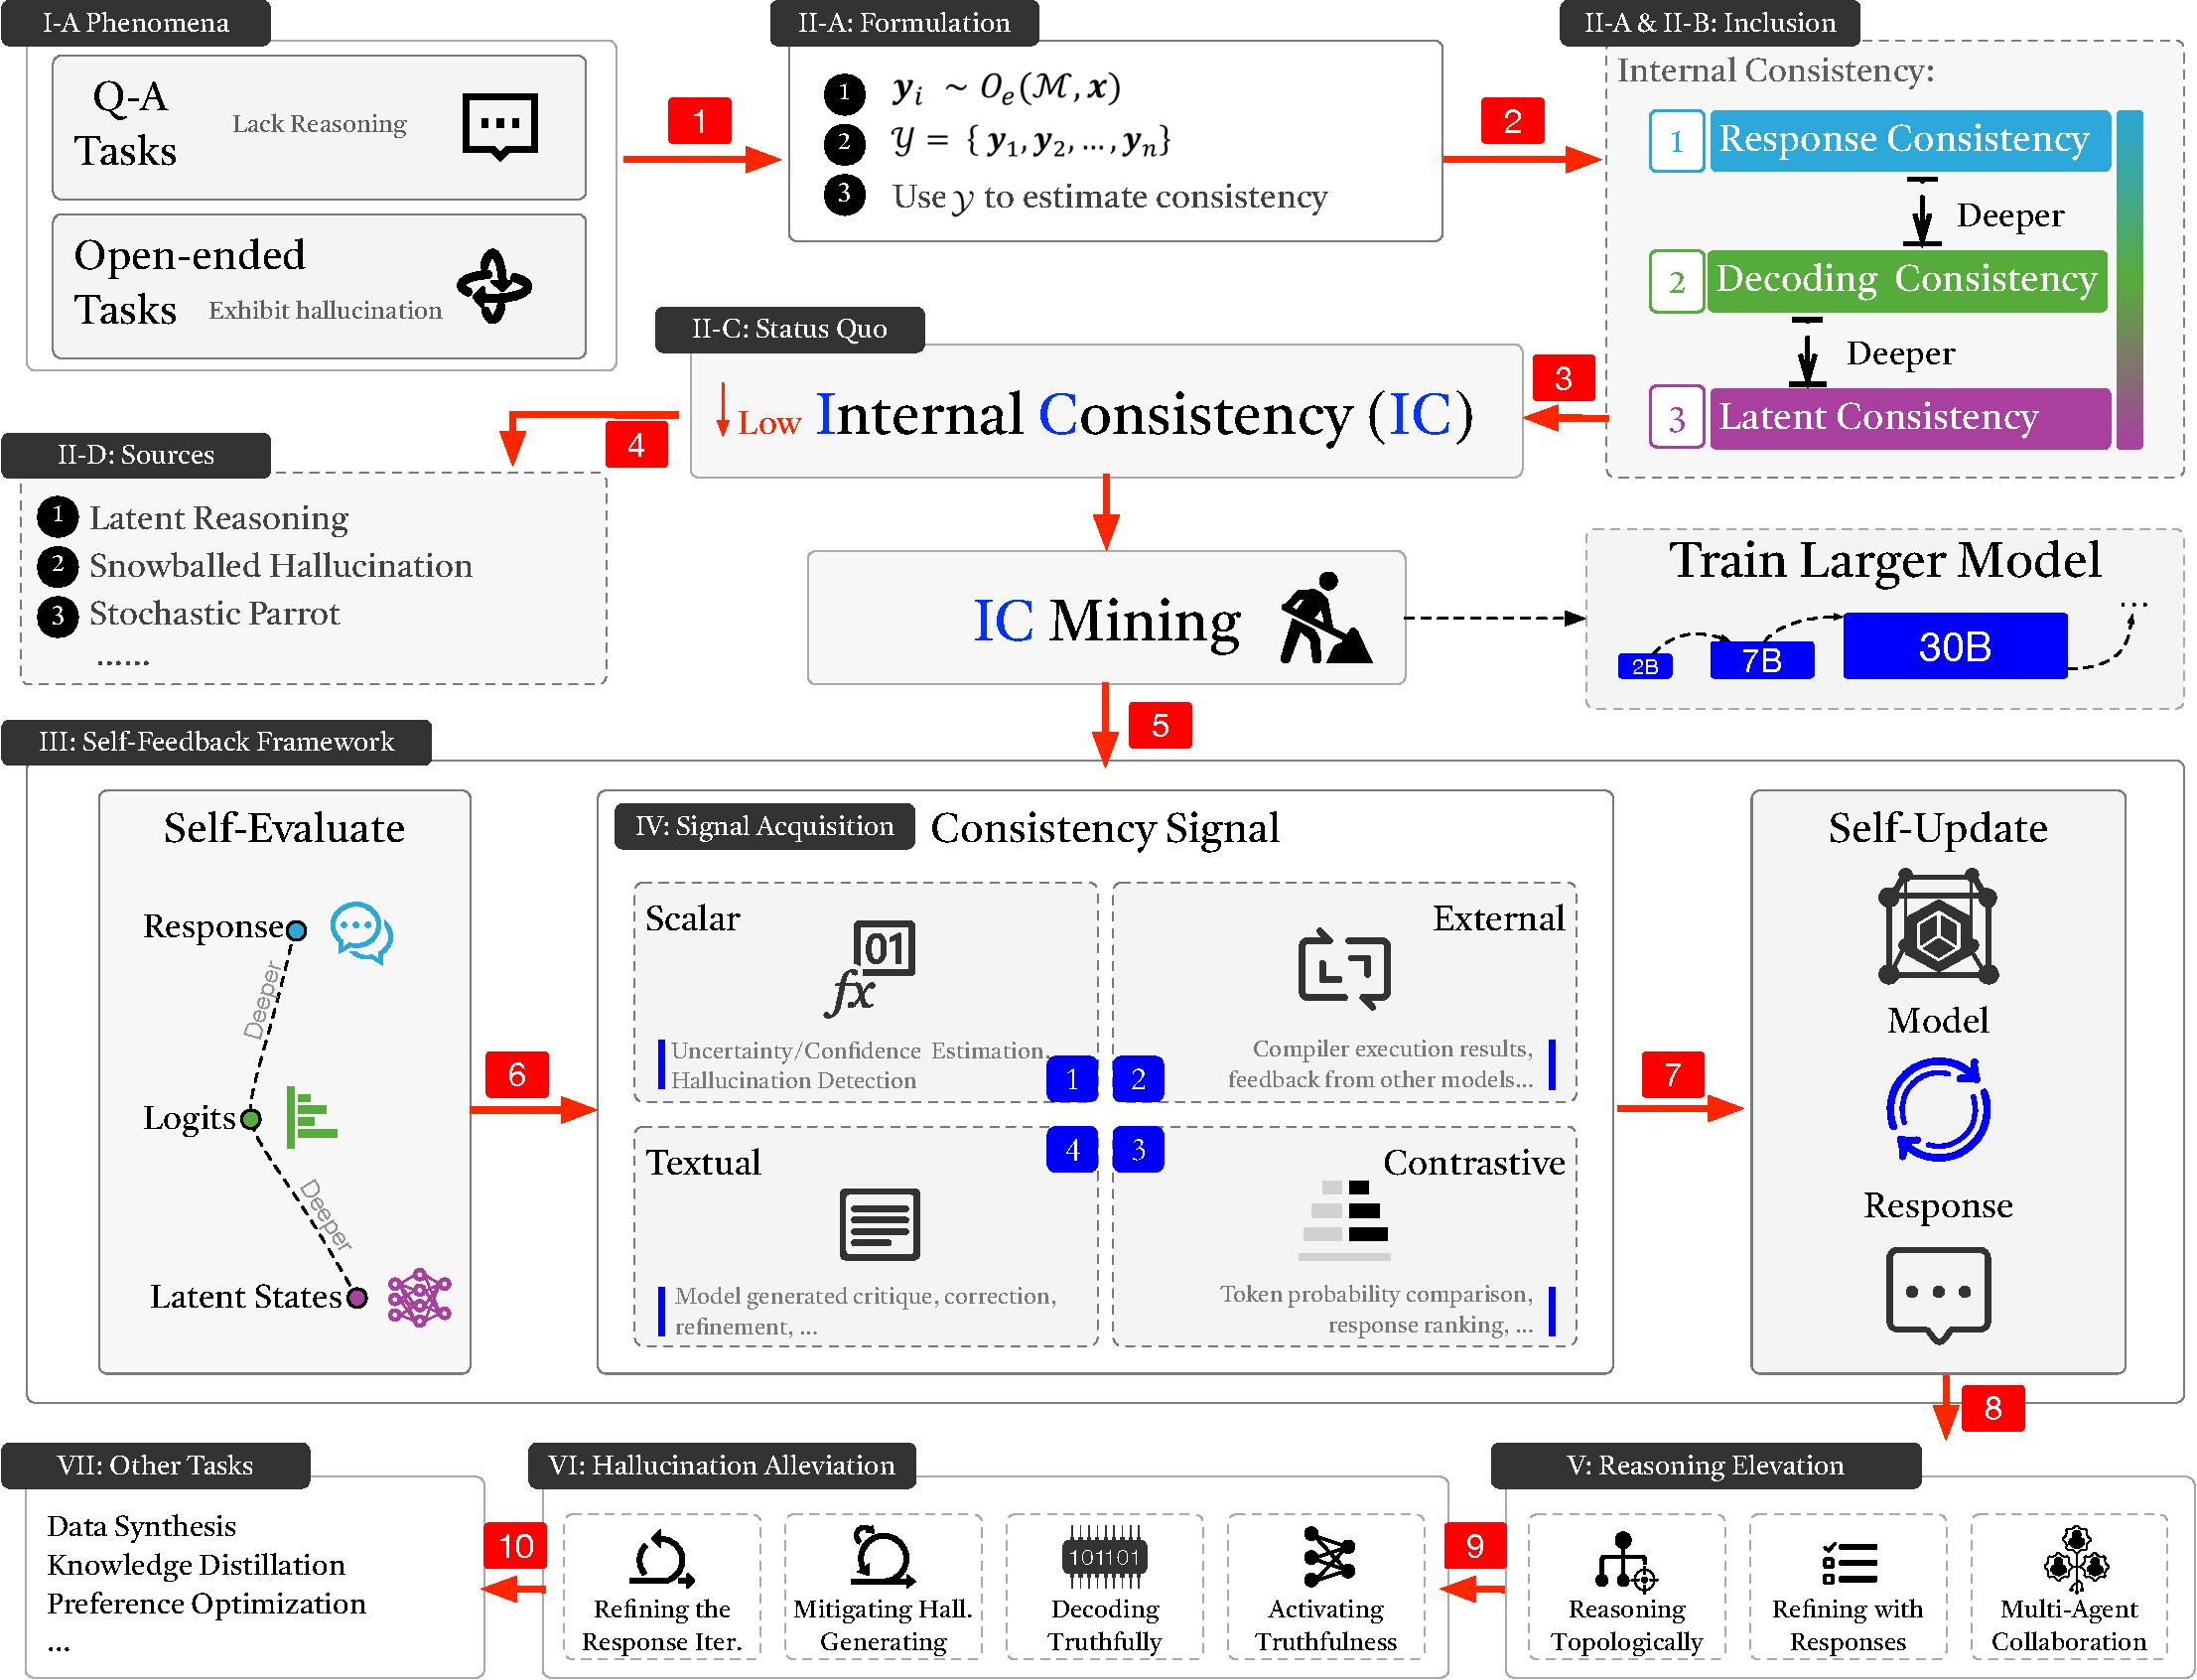
\includegraphics[width=\linewidth]{figures/article_framework.pdf}
    \caption{Core Concepts and Article Organization (Mainly Involving Sections~\ref{sec:internal_consistency} \~ ~\ref{sec:other_tasks}).}
    \label{fig:article_framework}
\end{figure*}


\subsection{Related Surveys}


\noindent Several other surveys have also focused extensively on works prefixed with ``Self-''. To our knowledge, surveys such as~\cite{SelfEvolution_24_arXiv_PKU}, ~\cite{SurveySelfCorrection_24_TACL_UCSB}, and ~\cite{SurveySelfCorrection_24_arXiv_PSU} demonstrate substantial similarities to our work. We present a straightforward comparison in Table~\ref{tab:related_surveys}.

\textit{A Survey on Self-Evolution of Large Language Models}~\cite{SelfEvolution_24_arXiv_PKU} primarily focuses on two aspects of literature. It covers articles on LLMs generating their own training data and papers employing multi-agent approaches for iterative optimization. Compared to other studies, this study is the most comprehensive in content. As shown in Table~\ref{tab:related_surveys}, the methods summarized in this survey encompass various tasks, including Instruction Following, Code Generation, and Planning. Given the wide range of tasks covered, the objectives of Self-Evolution proposed in this survey may lack a clear focus.

\textit{Automatically Correcting Large Language Models: Surveying the Landscape of Diverse Automated Correction Strategies}~\cite{SurveySelfCorrection_24_TACL_UCSB} specifically concentrates on Self-Correction, a process where models correct their own errors. Defined tasks encompass reasoning errors and harmful information. Owing to its explicit task definition, this survey offers a more detailed and comprehensive theoretical analysis. These tasks are classified based on the timing of correction, including training-time, generation-time, and post-hoc corrections. Although the classification approach is logical, it doesn't provide a comprehensive overview related to latent layers. Furthermore, the survey introduces a third task, Biased and Harmful Content Elimination, which is notably different from the first two tasks and leans towards subjective evaluation, indicating the potential for improvement in the task definition.

\textit{When Can LLMs Actually Correct Their Own Mistakes? A Critical Survey of Self-Correction of LLMs}~\cite{SurveySelfCorrection_24_arXiv_PSU} also focuses on Self-Correction, delving deeper into the issue by primarily questioning whether models can genuinely Self-Correct. However, the survey's approach to this question is limited as it only considers cases where Feedback Signals are textual and partially external, thereby directly constraining the scope of Self-Correction. Consequently, we find that the survey's summary is not sufficiently comprehensive and lacks adequate support for its conclusions. In Section~\ref{sec:does_it_work}, we further explore this issue and provide a more insightful analysis.

Compared to these surveys, our advantages are as follows:

\begin{enumerate}
    \item \textbf{Internal Consistency theoretical framework.} We offer an in-depth review of LLMs' Internal Consistency, examining its phenomena, formalization, status quo, etc. Furthermore, we introduce the task of Internal Consistency Mining, providing a unified perspective for reasoning elevation and hallucination alleviation tasks.
    \item \textbf{Self-Feedback theoretical framework.} Our framework includes Self-Evaluation, Consistency Signal Acquisition, and Self-Update. Characterized by its simplicity and comprehensiveness, this framework is poised to inspire further research. We summarize a broad array of Self-Evaluation strategies that extend from model responses to latent space exploration. These strategies allow us to capture a diverse range of Feedback Signals, extending beyond the scalar, textual, and external signals discussed in other surveys, to include contrastive signals.
    \item \textbf{Taxonomy based on lines of work.} Unlike other surveys that categorize methods based on theoretical frameworks alone, we organize similar methods into coherent lines of work. Subsequently, we summarize their Self-Evaluation and Self-Update strategies per line. Thus, our summarized lines are consistent with the baselines mentioned in related works, enabling scholars to quickly position their research within the field.
    \item \textbf{A better response to ``Does Self-Feedback Really Work?''} Many surveys discuss this question but often provide biased (using the success or failure of a specific method to represent the entire field) or overly complex (providing different answers for each type of work). analyses. Thanks to our proposed perspective on Internal Consistency, we provide a more insightful analysis.
\end{enumerate}

% 其他的相关综述
Additionally, we also incorporates insights from other weakly related surveys. Section~\ref{sec:uncertainty} draws inspiration from \cite{SurveyUncertainty_23_arXiv_Nankai}, which meticulously investigates the uncertainty issues in LLMs. Additionally, \cite{SurveyXofThought_24_arXiv_ETH} offers in-depth analyses of strategies like Chain of Thought, Self-Consistency, Tree of Thought, and Graph of Thought, which have guided our discussions in Section~\ref{sec:reasoning_topologically}. Moreover, the methodologies and insights from surveys on knowledge distillation~\cite{SurveyKD_24_arXiv_HKU} and preference learning~\cite{SurveyPL_24_arXiv_HIT} have been valuable in shaping Section~\ref{sec:other_tasks}.


\subsection{Structure of Our Work}


% 本文核心概念之间的逻辑和文章框架。
\noindent The logical structure and the organizational framework of this paper are depicted in Fig.~\ref{fig:article_framework}. Our research begins with the existing problem of low Internal Consistency in LLMs (Section~\ref{sec:status_quo}). Specific manifestations of low Internal Consistency include poor reasoning capabilities in question-answering (QA) scenarios and hallucinations in free-form generation (Section~\ref{sec:lack_reason_exhibit_hallu}). From a causal perspective, elements contributing to low Internal Consistency include inadequate latent reasoning abilities, the snowball effect of hallucinations, and the stochastic parrot hypothesis (Section~\ref{sec:sources_of_low}). We formalize internal consistency as the sampling-based consistency of model expressions across different layers (Section~\ref{sec:consistency_formulation}). This involves enhancing response consistency, decoding consistency, and latent consistency (Sections~\ref{sec:consistency_formulation} \&~\ref{sec:hourglass}).

To improve Internal Consistency, we propose Internal Consistency Mining across these layers. While scaling up the model is an intuitive solution, it comes with various cost-related challenges. Thus, we focus on the Self-Feedback theoretical framework, which mainly includes Self-Evaluation, Consistency Signal Acquisition, and Self-Update. Models obtain different forms of Internal Consistency signals through Self-Evaluation, and subsequently use these signals to Self-Update either responses or the model itself (Section~\ref{sec:self_feedback}). We explore six lines of work in Consistency Signal Acquisition (Section~\ref{sec:consistency_signal_acquisition}) and seven lines of work utilizing the Self-Feedback framework, divided into three lines dedicated to reasoning elevation (Section~\ref{sec:reasoning_elevation}) and four lines aimed at hallucination alleviation (Section~\ref{sec:hallucination_alleviation}).

Besides the central topics depicted in Fig.~\ref{fig:article_framework}, we have enriched Section~\ref{sec:other_tasks} with works that utilize the Self-Feedback framework, although not aimed at addressing low internal consistency. In Section~\ref{sec:evaluation}, we summarize relevant meta and common evaluation benchmarks and methods. Section~\ref{sec:does_it_work} delves into the question ``Does Self-Feedback really work?'' with an in-depth exploration, analyzing existing rebuttals and proposing appeals. Finally, Section~\ref{sec:future} outlines challenging research directions in the future.


\subsection{Out-of-scope Topics} \label{sec:out_of_scope}


\noindent To ensure the logical coherence and readability of this survey, we hereby clarify our discussion boundaries:

\begin{itemize}
    \item While this paper focuses on reasoning elevation and hallucination alleviation, we don't systematically review these aspects. Instead, we primarily discuss articles that utilize the Self-Feedback framework.
    \item The methods discussed in this paper aim to enhance the Internal Consistency. Although some methods may also employ the Self-Feedback framework, if their primary goal is not to improve Internal Consistency, they remain outside the scope. For example, DINO~\cite{DINO} focuses on generating datasets to train better Embedding models.
    \item The survey exclusively explores internal consistency and doesn't examine the interplay between internal and external consistencies. For instance, if a user maintains an opinion contrary to the LLM, should the LLM maintain its high internal consistency? This raises questions about the autonomy of models, which are profound but beyond our current scope. We proceed assuming agreement on correctness between the model and the user.
    \item Consistent with many related surveys summarizing methods whose names beginning with ``Self-'', our focus is on the model's self-awareness, self-assessment, self-correction, etc. The methods reviewed advocate for a model-in-the-loop approach, with minimal human intervention during the Self-Evaluation and Self-Update.
    \item Although retrieval-augmented generation (RAG) is notable for mitigating external hallucinations~\cite{gao2023retrievalaugmented}, this paper doesn't actively discuss RAG and primarily considers hallucinations caused by internal consistency to explore the limits of model honesty.
\end{itemize}


\section{Internal Consistency} \label{sec:internal_consistency}


\noindent Internal Consistency is the core concept in our work. In this section, we define this concept and present an experimental analysis that vividly delineates three distinct types of internal consistency. We discuss the strengths and weaknesses of current language models in terms of internal consistency and analyze their underlying reasons. Ultimately, we offer a straightforward explanation of internal consistency.


\subsection{Formulation} \label{sec:consistency_formulation}


\noindent Consistency is a critical term in logic, referring to a system where no two statements contradict each other~\cite{Tarski_1941}. However, systems like those of language models typically exhibit inconsistencies. For instance, as shown in Fig.~\ref{fig:inconsistent_responses}, even GPT-4o can't guarantee consistent responses to the same question. To better define the internal consistency, we utilize a sampling-based approach to model expressions in LLMs~\cite{SurveyUncertainty_23_arXiv_Nankai}\footnote{There are various methods to model the Internal Consistency, and the sampling-based perspective is a common one derived from the existing works. Important symbols discussed in this paper can be referred to in Appendix~\ref{apdx:notation}.}.

For a large language model $\mathcal{M}$ and a user query $\boldsymbol{x}$, we can obtain expressions from the model for this query, defined across three different types as follows:

\begin{itemize}
    \item \textbf{Expression from Response Layer (text).} Expressions consist of sentences that may show inconsistencies due to random sampling or subtle variations in input queries\footnote{Original: How many full stops (periods) are there: ``.!..!..!''; \\ Rewritten: How many full stops (periods) in the string below. \textbackslash n``.!..!..!'' \\ Just adding a ``\textbackslash n'' can lead to significant changes in the answer~\cite{sun2024evaluating}.}.
    \item \textbf{Expression from Decoding Layer (token).} Expression refers to the choice of different tokens influenced by various decoding strategies (e.g., beam search, top-p).
    \item \textbf{Expression from Latent Layer (vector).} Expression at this layer encompasses the different activation of attention heads and latent states across the model's architecture, contributing to diverse outputs. 
\end{itemize}

For the expression type $e$, the distribution of different expressions produced by model $\mathcal{M}$ in response to the query $\boldsymbol{x}$ can be defined as follows:

\begin{equation}
    O_e(\mathcal{M}, \boldsymbol{x}), \quad e \in \{\text{response}, \text{decoding},\text{latent}\}
    \label{eq:observation_distribution}
\end{equation}

By sampling from this distribution (e.g., repeatedly prompting the model with a query or its synonymous variants), we can obtain a sampling set with potentially repeated elements:

\begin{equation}
    \mathcal{Y}= \{ \boldsymbol{y}_1, \boldsymbol{y}_2, \ldots, \boldsymbol{y}_n \}, \quad \boldsymbol{y}_i \sim O_e(\mathcal{M}, \boldsymbol{x})
\end{equation}

Here, $\boldsymbol{y}_i$ represents the $i$-th sample obtained from $O_e(\mathcal{M}, \boldsymbol{x})$. With this sampling set, various methods can be employed to estimate the consistency of these expressions. For example, as shown in Fig.~\ref{fig:inconsistent_responses}, we can obtain $\mathcal{Y}= \{ 4,3,3,3,4 \}$. Below are two relatively trivial estimation methods. From a statistical perspective, we can compute the negative variance as a measure of consistency, as shown in Eq.~\ref{eq:dev}; from an information-theoretic perspective, we can use the negative entropy as a measure of consistency, as shown in Eq.~\ref{eq:info}. However, simple variance and entropy may not provide useful guidance for better result updates, and their applicability is limited to tasks where expressions are numerical labels.

\begin{equation}
    -D(\mathcal{Y})=-E(\mathcal{Y}-E(\mathcal{Y}))^2=-0.24
    \label{eq:dev}
\end{equation}

\begin{equation}
    -H(\mathcal{Y}) = \sum_{i=1}^n p(\boldsymbol{y}_i) \log_2 p(\boldsymbol{y}_i) \approx -0.971
    \label{eq:info}
\end{equation}

We will comprehensively discuss existing methods for acquiring consistency signals in Section~\ref{sec:consistency_signal_acquisition}.

Additionally, the three different types of ``expressions'' mentioned above constitute the main focus of this paper's discussion on three types of consistency: Response Consistency, Decoding Consistency, and Latent Consistency. Fig.~\ref{fig:consistency_type} visually illustrates the positions of these three types in an LLM.

\begin{figure}[t!]
    \centering
    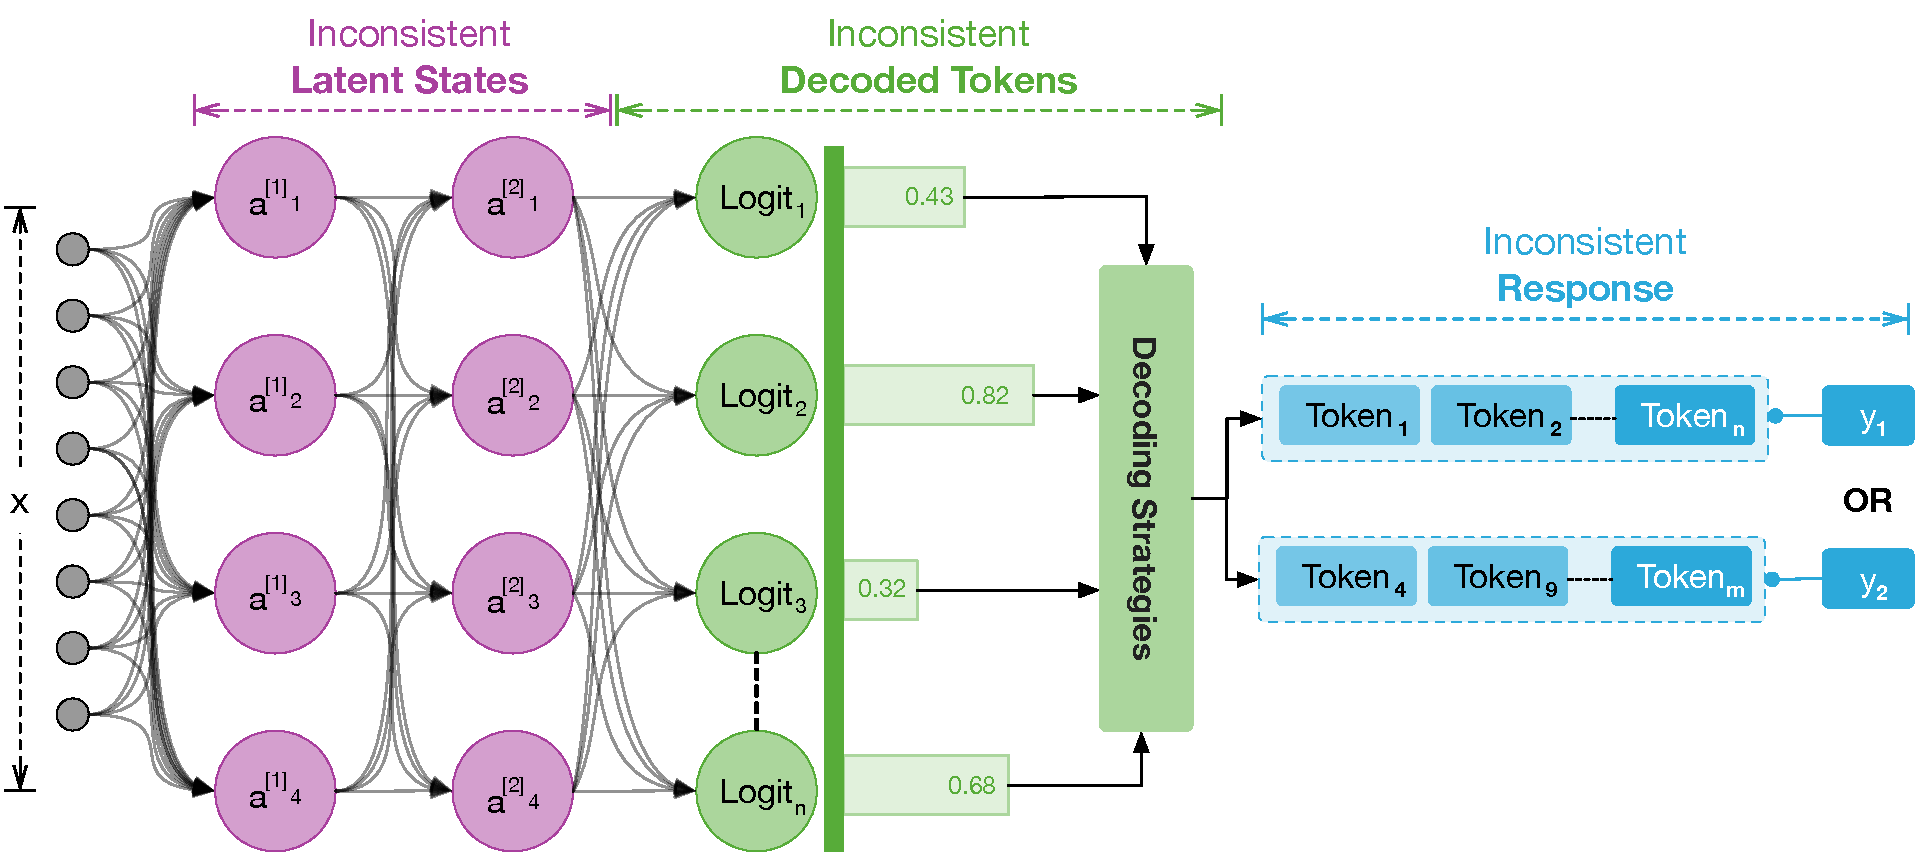
\includegraphics[width=\linewidth]{figures/consistency_type.pdf}
    \caption{Positions of the Three Types of Consistency}
    \label{fig:consistency_type}
\end{figure}


\subsection{The Hourglass Evolution of Internal Consistency}  \label{sec:hourglass}


\noindent In this section, we delve deeper into the three different types of Internal Consistency to uncover their relationships. We conducted a simple experiment where a model was asked to respond to a straightforward query to observe the consistency of different types of expressions. The given model $\mathcal{M}$ is Llama3-8B-Instruct\footnote{\url{https://ai.meta.com/blog/meta-llama-3/}}, and the given query $\boldsymbol{x}$ is: How many full stops (periods) are there: ``.!..!..!''. We then posed this question to the model to observe the preferred answers in the $\{\text{response}, \text{decoding}, \text{latent}\}$ layers. Below are the methods for collecting sampling sets at different layers. Refer to Appendix~\ref{apdx:experiment} for detailed experimental settings and results.

\textbf{Response Layer.} We used common Top-p sampling decoding with a temperature coefficient control to sample five times. To induce the model to output longer and more diverse content, we enabled CoT reasoning. We observed the model's final text choices during free generation. One example output is: ``Let's think step by step. There is one period at the end of the first part, then another after the second part, and finally one more after the third part. So, there are 3 periods in total.'' The resulting simplified sampling set is $\mathcal{Y}_\text{response} = \{ 5,3,3,3,3 \}$.

\textbf{Decoding Layer.} We used five decoding strategies to sample and observe the tokens selected. These decoding strategies included Greedy Decoding, Beam Search Decoding, Sampling Decoding, Top-k Sampling Decoding, and Top-p Sampling Decoding. The sampling set is $\mathcal{Y}_\text{decoding} = \{ 4,4,3,4,4 \}$.

\textbf{Latent Layer.} We hypothesized that different attention heads lead to different answers. To test this, we kept only the $h$-th attention head of the $l$-th Transformer block of model $\mathcal{M}$ active and set the attention output of other heads in that layer to zero, observing which token had the highest probability in the forward pass. We used six different combinations of $l$ and $n$, i.e., $(l,n) \in \{0, 15, 30\} \times \{0, 16\}$. The resulting ordered sampling set is $\mathcal{Y}_\text{latent} = < 0,0,5,4,4,4 >$\footnote{In this set, smaller $l$ are in front; for the same $l$, smaller $n$ are in front.}.

The experimental results are also shown in Fig.~\ref{fig:expt}. We observed that from the shallow layers of the latent layer to the deeper layers, through the intermediate decoding layer, and finally to the response layer, the consistency of the model's answers exhibits an ``hourglass evolution'' pattern.

\begin{figure}[t!]
    \centering
    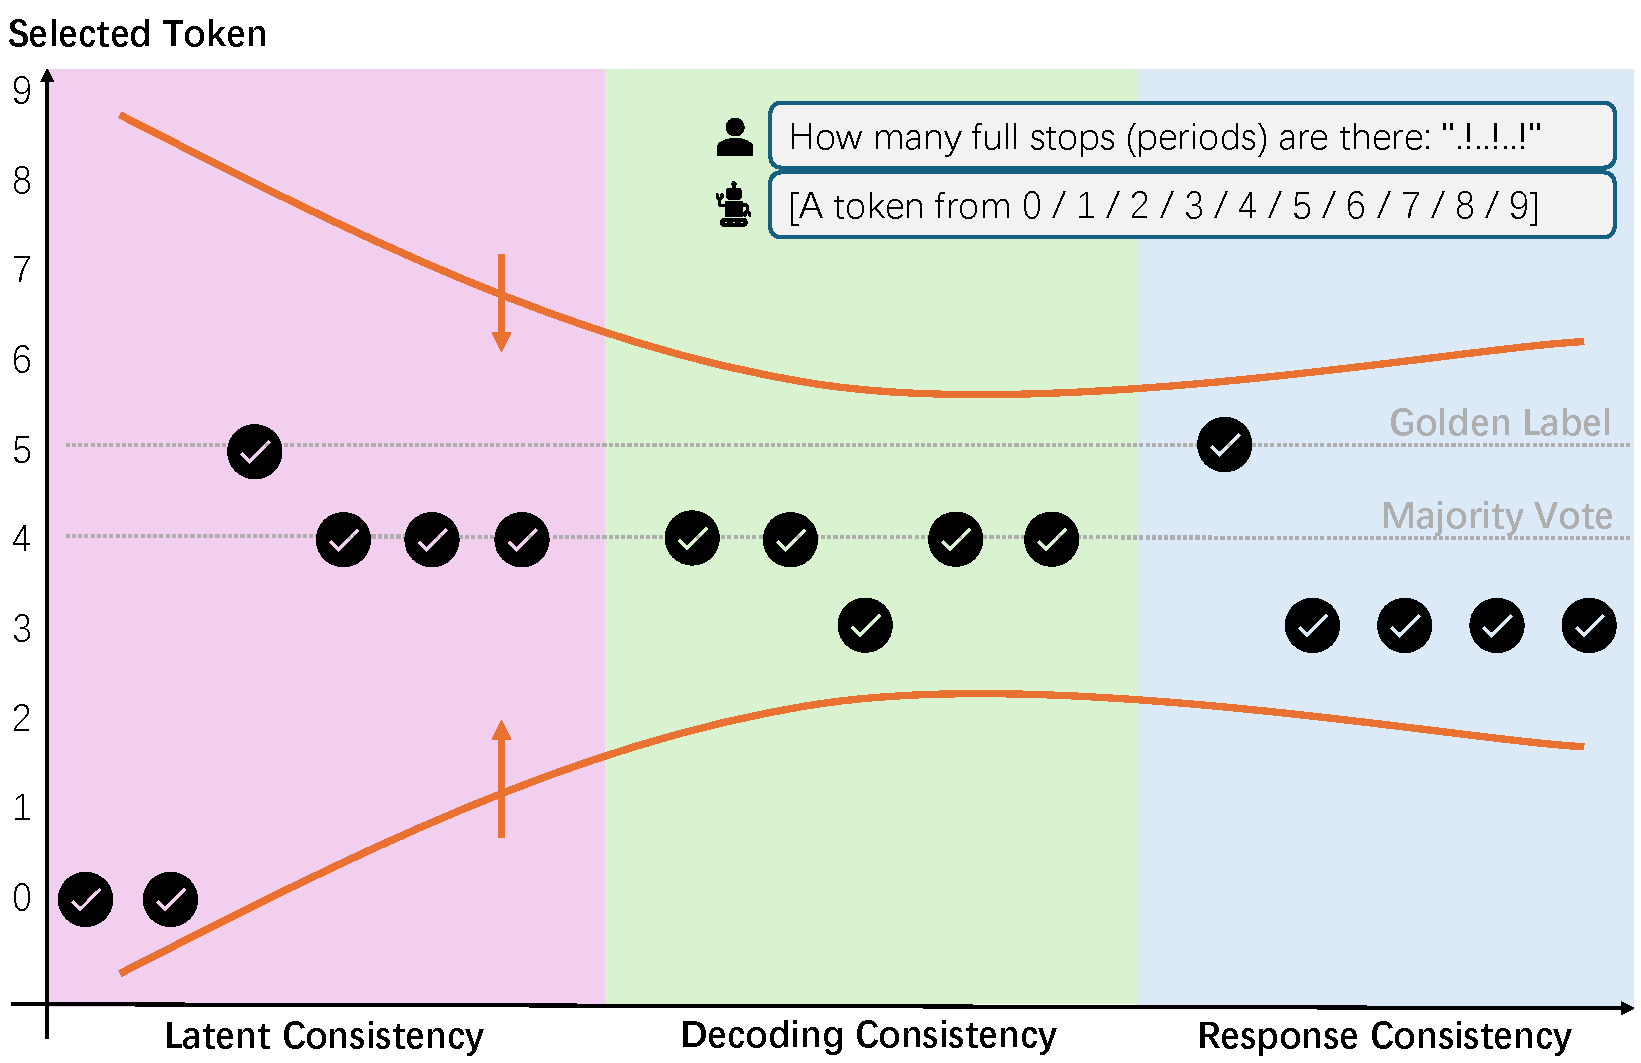
\includegraphics[width=\linewidth]{figures/inconsistency.pdf}
    \caption{The Hourglass Evolution of Internal Consistency}
    \label{fig:expt}
\end{figure}

We analyze this phenomenon as follows: In the latent state, since the forward propagation is not yet complete, the attention heads near the bottom layers may tend to choose answers randomly. In contrast, the attention heads near the top layers can continually accumulate knowledge from the previous layers due to the presence of residual connections, leading to a gradual convergence in judgment and increased certainty in answers. During the decoding phase, all decoding strategies tend to output the token with the highest probability, thus maintaining high certainty. However, at the response stage, greater variability appears. We believe this is because, when the LLM generates the first token, it has already conducted reasoning (latent reasoning\footnote{Yang et al.~\cite{TheoryLatentReason_24_arXiv_Google} introduce latent reasoning. This concept implies that when a Transformer model responds to a query, it has already conducted reasoning before generating the first token, similar to how humans think before speaking. We will also explain this concept further in Section~\ref{sec:sources_of_low}.}) and make an initial judgment of the answer. However, during the response phase, the output tokens such as ``I'm willing to help.'' can interfere with the model's initial reasoning and preliminary judgment, leading to a collapse in the computation results during latent reasoning.

From this figure, we can also see that our goal is to have the orange consistency boundary line move as close to the center as possible, which is the goal of internal consistency mining.


\subsection{Status Quo of LLM Consistency} \label{sec:status_quo}


\noindent This section briefly discusses the current performance of LLMs in terms of consistency. As indicated at the beginning of the survey, GPT-4o's various responses to the same question (see Fig.~\ref{fig:inconsistent_responses}) already demonstrate that even relatively powerful language models still exhibit low consistency.

There are also many works that either actively or inadvertently explore the Internal Consistency of LLMs. The well-known Self-Consistency~\cite{SelfConsistency_23_ICLR_Google} explores the use of the majority voting strategy, where the LLM generates multiple responses and selects the most voted one as the final response. Their experiments showed that on the reasoning benchmark GSM8K~\cite{cobbe2021training}, this method increased the answer accuracy from 56.5\% to 74.4\%. This implies that many responses may be random and do not represent a consistent response.

In terms of hallucination alleviation, M\"undle et al.~\cite{HalluSelfContradictory_24_ICLR_ETH} proposed the Self-Contradict strategy, which attempts to generate different samples to identify self-contradictory content and then eliminate these contradictions to reduce hallucinations. Their experiment showed that GPT-4, ChatGPT, Llama2-70B-Chat, and Vicuna-13B were able to induce self-contradictions at rates of 15.7\%, 17.7\%, 19.0\%, and 22.9\%, respectively.

Empirical tests show LLMs’ direct responses are inconsistent, even when they know the correct answer.

Besides response consistency, some works have explored whether models can consistently express what they know and do not know, a capability referred to as Self-Knowledge. For example, Yin et al.~\cite{TheoryKnowUnknown_23_ACL_Fudan} and Cheng et al.~\cite{TheoryKnowUnknown_24_arxiv_Fudan} created datasets consisting of questions that models cannot answer to test whether the models can refuse to answer these questions. Their research showed that models exhibit low consistency in refusing ``I Don't Know'' (IDK) questions, with room for improvement compared to humans.

Therefore, we believe the consistency of results obtained from LLMs using trivial forward propagation, trivial decoding strategies, and trivial model response strategies is low.


\subsection{Sources of Low Internal Consistency}  \label{sec:sources_of_low}


\noindent Why do models exhibit low consistency? Many scholars have conducted in-depth research on this phenomenon, exploring the causes from various angles such as prompt engineering, the decoding process, and the attention mechanism.

Some studies explore the impact of slight variations in prompts on response consistency. The structures of prompt may cause low consistency. Xie et al.~\cite{CalibIC_24_arXiv_SJTU} designed different CoT prompts and discovered that under different CoT's guidance, the latent state's distance between the intermediate and final layers of LLMs varied significantly. Simply put, some prompt designs result in low consistency between different latent layers, with significant differences in the probability distribution of the next token prediction. Liu et al.~\cite{LiTM_24_TACL_Stanford} tested the accuracy of LLMs' responses by placing text containing answers in different positions within the prompt, discovering a ``lost-in-the-middle'' phenomenon. Models tend to focus on the content at the beginning and end of prompts, leading to inconsistent responses to differently structured prompts. Similarly, Liu et al.~\cite{FFLM_23_NIPS_CMU} found that hallucinations emerge when LLMs dealing with long context. They analyzed that this is caused by the soft attention mechanism, where attention weights become overly dispersed as sequence length increases, leading to poor consistency in reasoning paths.

In addition to prompt engineering explorations, some researchers have directly investigated drawbacks within the LLM architecture. Yang et al.~\cite{TheoryLatentReason_24_arXiv_Google} studied whether models perform intermediate reasoning within latent states when answering questions and whether enhancing this intermediate reasoning signal strength could improve answer accuracy. Taking the example of the model answering ``In what year did Plato's teacher die?\footnote{Plato's teacher is Socrates, who died in 399 BC.}'', this work specifically investigated whether the model infers the intermediate entity ``Socrates'' in the latent layer and whether increasing the weight of the latent state corresponding to the intermediate entity would make the model answer more accurately. The experimental results showed that models do possess latent reasoning capabilities, but these are weak. On the one hand, the signal strength of the intermediate entity is weak. On the other hand, enhancing this signal strength did not significantly improve the LLM's response. This indicates deficiencies in current LLM architectures in performing and expressing latent reasoning. This means that when predicting the next token, the model may make near-random predictions due to failed intermediate entity reasoning. Additionally, Zhang et al.~\cite{TheorySnowball_23_arXiv_NYU} argued that models could appear hallucinations due to the ``snowball effect''. The full attention mechanism makes LLMs overly confident in their outputs, leading to compounding errors if an initial reasoning mistake occurs. Consequently, model's responses may become inconsistent with the knowledge it has learned.

Furthermore, some hypotheses and viewpoints reveal potential reasons for the low internal consistency of current LLMs. Bender et al.~\cite{Parrots_21_FAccT_UoW} proposed that large language models might be ``stochastic parrots'', learning rules and patterns from training data rather than truly understanding the grammar and semantics of natural language. This inherent randomness in generation reflects a form of internal inconsistency in the model. Ma et al.~\cite{PrincipleSC_22_FITEE} proposed the Principle of Self-Consistency for intelligent agents, aiming to find a coherent model that minimizes internal differences between observed and regenerated data. They found many factors that could affect internal consistency, such as mode collapse\footnote{Mode collapse: A generative model starts producing very similar or repetitive outputs during training, failing to capture the diversity of the data.}, neural collapse\footnote{Neural collapse: The model learns the simplest representation to map input to output, without capturing the complex logic within the data.}, and over-fitting or under-fitting caused by overly high or low dimensional feature spaces.

In conclusion, both theoretical and experimental findings indicate that model architecture, training processes, and user's queries can all contribute to low internal consistency. Understanding these causes can help researchers better address this issue and improve model performance.

% 未来可能可加的:
% 不可自我认识:无法检查自己的logit
% 幻觉是人类语言的本质,我们依赖幻觉


\subsection{How to Understand Internal Consistency?}


\noindent This section adopts a broader perspective, an alignment perspective, to help readers understand Internal Consistency. If there is Internal Consistency, there must also be corresponding External Consistency. Internal Consistency focuses on whether the model can align with itself during expression. External Consistency includes the alignment between the pre-training dataset and the pre-training model parameters, the alignment between the pre-trained model and the chat model, and the alignment between the chat model and the model subjected to RLHF (Reinforcement Learning with Human Feedback), among others. These different alignments can be illustrated in Fig.~\ref{fig:full_consistency}. Each stage of alignment plays a unique role. Internal Consistency is crucial for AI safety. Kadavath et al.~\cite{TheoryKnowKnow_22_arXiv_Anthropic} mention the significant value of Internal Consistency:

\begin{figure*}[t!]
    \centering
    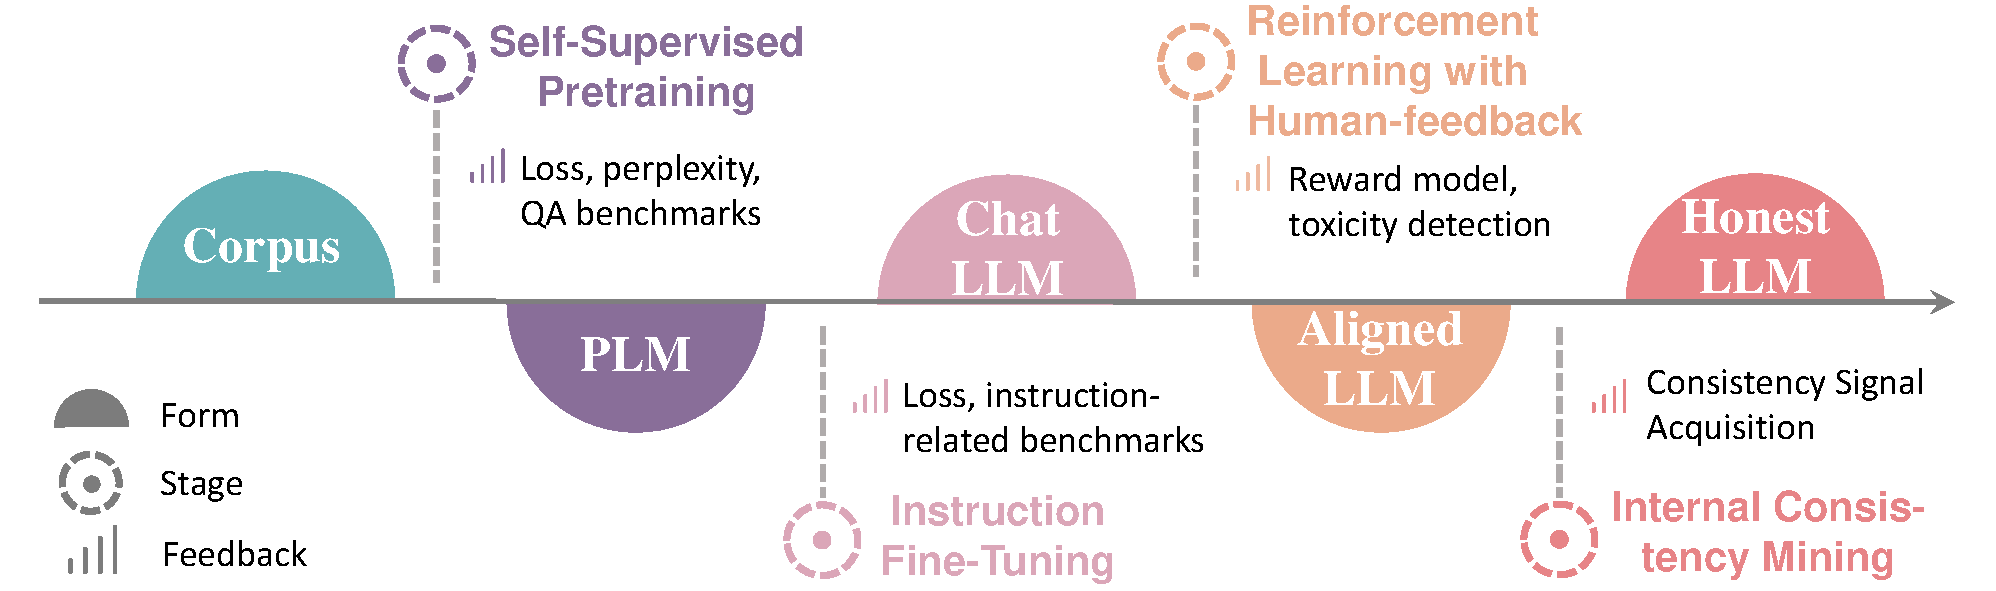
\includegraphics[width=\linewidth]{figures/full_consistency.pdf}
    \caption{Various Alignments Involved in the LLM development}
    \label{fig:full_consistency}
\end{figure*}

\begin{itemize}
    \item \textbf{Truthfulness.} LLMs should provide factually accurate information, including finding, using, and evaluating source materials correctly.
    \item \textbf{Calibration.} LLMs' probabilistic predictions should correspond with frequencies of occurrence.
    \item \textbf{Self-Knowledge.} LLMs should know what they know and make accurate predictions about their own behavior.
    \item \textbf{Explainability.} LLMs should reveal their ``thinking'' completely and faithfully.
    \item \textbf{Non-deceptiveness.} LLMs should be ensured not to lie, even when human preference might encourage systematic mistakes or provide rewards for pleasant misconceptions.
\end{itemize}

In addition to these significant values in AI safety, Internal Consistency also affects the robustness and reliability of AI systems. For instance, the current inability of models to reason consistently directly impacts an AI agent's understanding of goals, leading to incorrect operations by the agent~\cite{han2024llm}.


\section{Self-Feedback Framework} \label{sec:self_feedback}


\subsection{Formulation}


\noindent Self-Feedback is a theoretical framework we have summarized from numerous studies. It includes Self-Evaluation and Self-Update, as shown in the middle part of Fig.~\ref{fig:article_framework}.

\begin{tcolorbox}[colback=white!98!black,colframe=white!30!black,boxsep=1.1pt,top=6.75pt]%
\vspace{1.75pt}%
\textbf{Self-Feedback}\\[-0.575em]
\noindent\makebox[\textwidth]{\rule{\textwidth}{0.4pt}}
\\[0.25em]
Narrowly speaking, Self-Feedback refers to the method of improving a model's own Internal Consistency through its feedback, where ``own'' refers to a specific model entity or a specific response. \\
\\
Broadly speaking, ``own'' can be extended to other models. For example, multiple different models can improve their capabilities through feedback generated from debates among them, which is a more generalized interpretation of Self-Feedback.
\end{tcolorbox}

Based on the above descriptive definition, we can formalize the process of Self-Feedback. For a given model $\mathcal{M}$, query $\boldsymbol{x}$, and a sampling set $\mathcal{Y}$ obtained under a certain expression, Self-Evaluate\footnote{A small number of methods use other models $\text{SelfEvaluate}_\mathcal{N}(\mathcal{Y})$ or even external tools $\text{SelfEvaluate}_\text{tool}(\mathcal{Y})$ during Self-Evaluate.} is first performed to obtain feedback $f$:

\begin{equation}
    f = \text{SelfEvaluate}_\mathcal{M}(\mathcal{Y})
    \label{eq:selfevaluate}
\end{equation}

We can use the obtained feedback $f$ to let the model $\mathcal{M}$ directly update the original expression $\mathcal{Y}$ to $\boldsymbol{y}'$:

\begin{equation}
    \boldsymbol{y}'=\text{SelfUpdate}_\mathcal{M}(\mathcal{Y}, f)
    \label{eq:selfupdate1}
\end{equation}

We can also use the obtained feedback $f$ to select better responses and optimize the model parameters $\mathcal{M}$ through fine-tuning or other strategies to obtain a better model $\mathcal{M}'$:

\begin{equation}
    \mathcal{M}'=\text{SelfUpdate}_\mathcal{M}(\mathcal{Y}, f)
    \label{eq:selfupdate2}
\end{equation}

Additionally, we can use the feedback to update other models, such as updating a student model $\mathcal{N}$:

\begin{equation}
    \mathcal{N}'=\text{SelfUpdate}_\mathcal{N}(\mathcal{Y}, f)
    \label{eq:selfupdate3}
\end{equation}

The combination of Self-Evaluate defined in Eq.~\ref{eq:selfevaluate} and Self-Update defined in Eqs.~\ref{eq:selfupdate1}, \ref{eq:selfupdate2}, and \ref{eq:selfupdate3} constitutes various Self-Feedback methods. During Self-Evaluate, external signals may be used, and during Self-Update, other models may be updated. This interaction with external entities is referred to as generalized Self-Feedback.


\subsection{Taxonomy}


\noindent The Self-Feedback methods introduced in this paper can be categorized from two different perspectives, as shown in the middle and bottom parts of Fig.~\ref{fig:article_framework}.

The first perspective classifies based on the components of Self-Feedback, as depicted in the middle part of Fig.~\ref{fig:article_framework}. In Self-Feedback, the initial step is Self-Evaluation. The model can evaluate its own response, token probability distribution, or the latent states. Through Self-Evaluation, different consistency signals can be obtained: scalar signals (e.g., the confidence level of the output), textual signals (e.g., the model's critique of its own output), external signals (e.g., results from a Python interpreter), and comparative signals (e.g., different token probability distributions induced by two different prompts). These signals are then used for downstream Self-Update, with three typical update strategies. The model can use the signals to prompt itself for direct result modification, identify better outputs for re-tuning itself through Self-Evaluation, or even re-tune a student model in the domain of knowledge distillation using better outputs. Theoretically, this yields a total of $3\times4\times3=36$ method combinations. Obviously, the drawback of this taxonomy is its excessive granularity and lack of task-oriented perspective, which make it difficult for researchers to design new solutions for specific task.

To avoid the shortcoming, we primarily adopt the second perspective, categorizing based on the tasks and lines of work, as illustrated at the bottom of Fig.~\ref{fig:article_framework}. Firstly, the major challenge for LLMs is low Internal Consistency. To address this, it is essential to clarify what the intermediate consistency signals are and how they are acquired. In Section~\ref{sec:consistency_signal_acquisition}, we summarize six important lines of work.

In terms of specific manifestations, low Internal Consistency includes two major issues: weak reasoning ability in QA tasks and hallucinations in open-ended generation. Therefore, in Section~\ref{sec:reasoning_elevation}, we summarize three lines of work for Reasoning Elevation. And in Section~\ref{sec:hallucination_alleviation}, we summarize four lines of work for Hallucination Alleviation. Table~\ref{tab:reason_hall_paradigms} summarizes these seven lines of work. Additionally, some tasks do not aim to improve consistency but still utilize the Self-Feedback framework. For comprehensiveness, we also briefly summarize these other tasks in Section~\ref{sec:other_tasks}.

\begin{table*}[h!]
\begin{threeparttable}

\caption{Different Lines of Work in Reasoning Elevation and Hallucination Alleviation}
\label{tab:reason_hall_paradigms}
\scriptsize
\begin{tabular}{p{2.4cm}p{1.3cm}p{2.1cm}p{0.8cm}p{0.5cm}p{1.65cm}p{1.5cm}p{3.85cm}}
\toprule
\textbf{Section: Paradigm}  &  \textbf{Expression}     & \textbf{Signal Type}                    & \textbf{\#LLM}  &\textbf{Train.} & \textbf{Self-Evaluation}                     & \textbf{Self-Update}                   & \textbf{Typical Works}                        \\
\midrule
\ref{sec:reasoning_topologically}: Reasoning Topologically                  & Response, \newline Decoding & Scalar, Textual, \newline Contrastive   & 1      & No         & Majority Voting, Value Function & Best Selection                & Self-Consistency~\cite{SelfConsistency_23_ICLR_Google}, ToT~\cite{ToT_23_NeuIPS_Princeton}, GoT~\cite{GoT_24_AAAI_ETH}           \\
\midrule
\ref{sec:refining_with_responses}: Refining with Responses                  & Response            & Textual                        & 1 or 2 & Half            & Sampling                            & Best Selection, Model Tuning & Self-Improve~\cite{SelfImprove_23_EMNLP_Illinois}, ConCoRD~\cite{ConCoRD_22_EMNLP_Stanford}, LEMA~\cite{LearnMistake_24_arXiv_MS}          \\
\midrule
\ref{sec:multi_agent}: Multi-Agent Collaboration                             & Response            & Textual, Scalar                & $\geq 2$     & Rare   & Negotiation                         & Answer Aggregation            & FORD~\cite{ModalCollaboration_23_EMNLP_HIT}, MACNet~\cite{MACNet_24_arXiv_THU}, REFINER~\cite{REFINER_24_EACL_EPFL}                \\
\midrule
\midrule
\ref{sec:refining_the_response_iteratively}: Refining the Response Iteratively        & Response            & Textual, External              & 1      & Few           & Model Generate Critique             & Model Generate Refinement     & Self-Refine~\cite{SelfRefine_23_NeuIPS_CMU}, Reflexion~\cite{Reflexion_23_NeuIPS_Northeastern}, Self-Correct~\cite{SelfCorrect_23_ICLR_AI2} \\
\midrule
\ref{sec:mitigating_hallucination_while}: Mitigating Hallu. while Generating & Response            & Textual, Contrastive, \newline External & 1      & Few            & Inherent model evaluation           & Model Delete Hallucination    & Self-Contradict~\cite{HalluSelfContradictory_24_ICLR_ETH}, EVER~\cite{EVER_arXiv_23_UNC}, FEVA~\cite{FAVA_24_arXiv_Washington}       \\
\midrule
\ref{sec:decoding_truthfully}: Decoding Truthfully                    & Decoding            & Contrastive                    & 1 or 2 & No            & Evaluate Decoding Path               & Select the Best Decoding Path & DoLa~\cite{DoLa_24_ICLR_MIT}, CAD~\cite{ContextAwareD_23_arXiv_Washington}, DIVER~\cite{DIVER_24_arXiv_IA}, SED~\cite{SED_24_arXiv_FDU}                      \\
\midrule
\ref{sec:activate_truth}: Activating Truthfulness                 & Latent              & Contrastive                    & 1      & No            & Evaluate Latent States              & Activate the Best States      & ITI~\cite{ITI_23_NeuIPS_Harvard}, TrFr~\cite{TrFr_24_AAAI_BUAA}, TruthX~\cite{TruthX_24_ACL_ICT}               \\
\bottomrule
\end{tabular}

\begin{tablenotes}
\footnotesize
\item \textit{Note}: This table summarizes the characteristics of representative methods. The first three lines are dedicated to ``Reasoning Elevation'', while the latter four lines are focused on ``Hallucination Alleviation.'' \#LLM indicates the number of LLMs needed. Train. denotes ``How many works need training?''
\end{tablenotes}


\end{threeparttable}
\end{table*}
% TODO:删除掉了Inference cost,未来可以考虑使用inference-time time complexity和inference-time space complexity来代替。或者单独添加一个推理次数,表示生成多少次响应。


\section{Task: Consistency Signal Acquisition} \label{sec:consistency_signal_acquisition}


% 概念
\noindent Consistency signal acquisition refers to evaluating the consistency of expressions after obtaining the sampling set $\mathcal{Y}$ from the language model $\mathcal{M}$ for the query $\boldsymbol{x}$. The evaluated signal can help the model update its expressions or parameters, thereby improving the model's Internal Consistency. Therefore, consistency signal acquisition is a pivotal task within the Self-Feedback framework. These methods either require access only to the model's output contents, to the logits, or the latent states of the model. Depending on the depth of access required by different methods, the approaches mentioned in this section are categorized as black-box (accessing only the model's output contents), gray-box (also accessing logits), and white-box (also accessing the model's latent states). Numerous explorations have been undertaken in this task. These include:

\begin{itemize}
    \item Section~\ref{sec:uncertainty}: Uncertainty Estimation (Scalar)
    \item Section~\ref{sec:confidence}: Confidence Estimation (Scalar)
    \item Section~\ref{sec:hallucination}: Hallucination Detection (Scalar)
    \item Section~\ref{sec:critiquing}: Verbal Critiquing (Textual)
    \item Section~\ref{sec:contrastive_optimization}: Contrastive Optimization (Contrastive)
    \item Section~\ref{sec:external_feedback}: External Feedback (External)
\end{itemize}
% TODO 高优先级:我们把这些工作线也总结在了表xxx中。字段包括:透明性(黑白灰盒),#llm,reference-free,计算公式,计算目标(uncertainty,confidence,hallucination等),基于sample与否等

% \textbf{uncertainty estimation} derived from the traditional machine learning era, modern model response \textbf{confidence estimation}, finer-grained \textbf{hallucination detection}, and non-scalar but textual \textbf{verbal critiquing}. There are also broader or relatively implicit types such as \textbf{contrastive optimization} and \textbf{external feedback}.


% 前三条工作线的联系与区别
The names of the first three lines of work mentioned above separate research topics that are actually quite similar. They all provide scalar feedback for LLM responses, and some works even mix the keywords from these three lines, such as \cite{Uncertainty_21_EACL_UCSB, Uncertainty_24_TMLR_Illinois, BelieveOrNot_24_arXiv_Google}. The differences among these three lines mainly lie in the slight distinctions in their downstream tasks. Estimating the uncertainty and confidence of model expressions is essentially two sides of the same coin, as both calculate the model's certainty level to obtain a scalar within the range of $[0,1]$. This approach is often used to optimize the model's reasoning ability, selecting a better reasoning path based on the uncertainty rate or confidence rate. Moreover, hallucination detection determines the presence of hallucinations (choosing from $\{0, 1\}$) through various methods, which is evidently more used in the task of hallucination alleviation.

% 后三条工作线
In addition to the aforementioned works that obtain scalar signals, other types of signals have been explored. Verbal Critiquing refers to having the language model directly evaluate the quality of an output, providing suggestions for improvement. External Feedback leverages external sources, such as textual feedback from other robust models or error messages from a compiler in code generation tasks. Finally, there is a more implicit signal, contrastive optimization, which obtains consistency signals through the comparison between different expressions and optimizes towards consistency.

% 讲解范围
In this section, we focus more on the first three lines of work, as they are often studied independently and are hotspots in academic research. The last three lines of work are only briefly mentioned here, as they tend to be relatively simple or implicit methods. They will be elaborated in Sections~\ref{sec:reasoning_elevation},~\ref{sec:hallucination_alleviation}.


\subsection{Uncertainty Estimation} \label{sec:uncertainty}


% 定义
\noindent Due to the black-box nature of the deep learning, uncertainty estimation has always been an important topic. Uncertainty estimation refers to estimating the data uncertainty, model uncertainty, and distributional uncertainty involved in the neural networks~\cite{deng2023uncertainty}. For uncertainty estimation in the NLP field, Hu et al.~\cite{SurveyUncertainty_23_arXiv_Nankai} conducted a detailed survey. Interested readers can refer to this article for further understanding. Here we briefly introduce the uncertainty modeling proposed in their work.

% 不确定性的建模/来源
The purpose of uncertainty modeling is to identify the sources of uncertainty that cause the model to generate uncertain results and to systematically understand the uncertainties present in the model. Hu et al.~\cite{SurveyUncertainty_23_arXiv_Nankai} categorize and explain the sources and modeling methods of uncertainty from the perspectives of models, outputs, and distributions. 1) \textbf{Calibration Confidence-based Methods}: This approach aims to correct the reliability of the uncertainty estimates provided by the model. The basic idea is to compare the accuracy of predicted probabilities with actual probabilities. 2) \textbf{Sampling-based Methods}: This approach models the variability of multiple expressions provided by the model, allowing us to observe the arising uncertainties. This method is also the focus of our article. 3) \textbf{Distribution-based Methods}: This approach starts with the training dataset, pre-judging the distribution characteristics of the dataset and directly calculating the model's inherent uncertainty by constructing specific distribution functions.

% MCD方法
We introduce an important method cluster within Sampling-based Methods: Monte Carlo Dropout (MCD)~\cite{pmlr-v48-gal16}. In traditional deep learning, model predictions are often deterministic, and multiple samples yield consistent answers, preventing us from understanding the model's implicit certainty about the results. The MCD method uses dropout technique to construct an implicit binomial distribution. For example, a 50\% dropout probability constructs a $ B(\text{\#activation}, 0.5)$ binomial distribution, which implicitly creates multiple models with different parameters $\theta_i \sim q(\theta), i=1,2,\ldots,n$. At test time, MCD uses multiple models with different parameters to obtain multiple output results $P(\boldsymbol{y}_i | \boldsymbol{x}; \theta_i)$ and estimates the model's uncertainty by calculating the variance of results. As for LLM, obtaining different expressions is much easier, such as using temperature coefficients to control generation. From the perspective of MCD, changing the probability of the Softmax layer implicitly constructs different models.

% 简单的方法
Besides MCD, which offers more explanatory insights, there are simpler, Sampling-based Methods available. For example, the Active Prompting strategy proposed by~\cite{ActivePrompt_23_arXiv_HUST} uses disagreement in answers as an estimate of uncertainty, $\text{SelfEvaluate}(\mathcal{Y}) \triangleq \frac{|\text{unique}(\mathcal{Y})|}{|\mathcal{Y}|}$. Here, $\text{unique}(\mathcal{Y})$ represents the set after removing duplicate elements.

% TODO 不重要目前 如果要加更多文献,uncertainty综述里,还有active prompting文章里还有很多内容可选


\subsection{Confidence Estimation} \label{sec:confidence}

% 引入
\noindent Literally, confidence is just the antonym of uncertainty, and their evaluation objectives are the opposite. Uncertainty tends to provide insights into model interpretability, while confidence focuses on providing reliability scores, thereby directly enhancing user trust and engagement with the responses.

% 重点方法阐述
In this line of work, Self-Evaluation is the core method\footnote{The Self-Evaluation here denotes the method proposed in~\cite{TheoryKnowKnow_22_arXiv_Anthropic}, not the Self-Evaluation in Self-Feedback framework. To distinguish between the two, citation markers will be appended when referring to the method.}. The concept of Self-Evaluation was first proposed in~\cite{TheoryKnowKnow_22_arXiv_Anthropic}, where the goal is for the model to express its level of confidence using its own knowledge and reasoning. As shown in Fig.~\ref{fig:prompt_for_self_eval}, the Self-Evaluation method simply asks the AI: Is the proposed answer True or False? Then, the confidence score, P(True), is extracted from the model's logits.

\begin{figure}[h!]
\centering

\begin{tcolorbox}[colback=blue!5!white,colframe=blue!75!black,title=Prompt for Self-Evaluation,fontupper=\footnotesize,fonttitle=\scriptsize]
\textbf{Question}: Who was the first president of the United States? \\
\textbf{Proposed Answer}: George Washington was the first president. \\
\textbf{Is the proposed answer}: \\
(A) True \\
(B) False \\
\textbf{The proposed answer is}:
\end{tcolorbox}

\caption{Prompt for Self-Evaluation~\cite{TheoryKnowKnow_22_arXiv_Anthropic}}
\label{fig:prompt_for_self_eval}
\end{figure}

Besides naively asking the model whether it thinks the proposed answer is correct, some works have proposed other frameworks. For instance, BSDetector~\cite{TheoryUncertainty_23_arXiv_UoMaryland} is a confidence estimation framework suitable for both black-box and white-box models. It combines the consistency of multiple outputs sampled from the model with model's own reflection on its output, weighting these scores to obtain the confidence scores. Another example, TrustScore~\cite{TrustScore_24_arXiv_UoEdinburgh} is a reference-free confidence estimation framework using behavior consistency. It generates distractors based on entity information rules from Wikipedia, asks the LLM multiple times, and checks if it consistently chooses its own generated answer.


\subsection{Hallucination Detection} \label{sec:hallucination}


% TODO: 缺少介绍段落
\noindent Hallucination Detection aims to identify untruthful or unfaithful text within a response.  SelfCheckGPT~\cite{HalluSelfCheckGPT_23_EMNLP_Cambridge} provides a reference-free hallucination detection framework. Specifically, the goal of SelfCheckGPT is to determine the presence of hallucination in a given query $\boldsymbol{x}$ and response $\boldsymbol{y}_0$. The framework works in three steps. Firstly, the model samples several different responses, $\mathcal{Y}= \{\boldsymbol{y}_1, \boldsymbol{y}_2, \ldots, \boldsymbol{y}_n \}$. Secondly, it calculates whether $\boldsymbol{y}_{1:n}$ support $\boldsymbol{y}_0$. Finally, it summarizes the support level to calculate the final score. Designing support level metric is where creativity can be applied, and the authors provide five different methods:

\begin{itemize}
    \item \textbf{Similarity-based}: Compute the negation of the mean similarity between $\boldsymbol{y}_{1:n}$ and $\boldsymbol{y}_0$;
    \item \textbf{QA-based}: Generate many questions from $\boldsymbol{y}_0$ and test consistencies in the answers derived from $\boldsymbol{y}_0$ and $\boldsymbol{y}_{1:n}$;
    \item \textbf{N-gram model-based}: Build an n-gram model from $\mathcal{Y}$, then use it to compute the negation of the mean transition probability between tokens in $\boldsymbol{y}_0$.
    \item \textbf{Natural language inference (NLI)-based}: Compute the mean probability of contradiction between the responses;
    \item \textbf{Prompt-based}: Similar to Self-Evaluation~\cite{TheoryKnowKnow_22_arXiv_Anthropic}, directly ask the language model whether $\boldsymbol{y}_{1:n}$ support $\boldsymbol{y}_0$.
\end{itemize}

The Alibaba team proposed INSIDE~\cite{INSIDE_24_ICLR_Alibaba} for deeper exploration. They sampled the latent expressions. They extracted the vectors from the intermediate layers corresponding to the last token of the sampled sentences and calculated the covariance matrix of these vectors. Since the eigenvalue of the covariance matrix represents data variability, they used this value as a measure of hallucination. Intuitively, if the variability is small, it indicates that the sentence vectors are not far apart from each other, and the likelihood of hallucination is low.

The above works generally employ a single LLM. Additionally, some methods utilize multiple agents to detect hallucination. For example, Cross Examination~\cite{CrossExamine_23_EMNLP_TAU} uses two LLMs, an Examinee, and an Examiner, employing a cross-examination approach to determine factual errors. The Examinee generates responses, while the Examiner iteratively asks questions related to the initial response. The Examinee answers these questions for several rounds, then examiner determines whether there are factual errors.


\subsection{Verbal Critiquing}  \label{sec:critiquing}


\noindent The aforementioned methods can only provide scalar signals for downstream Self-Update, lacking flexibility. Inspired by the idea that ``all tasks are generation tasks''~\cite{BARTScore_21_NeuIPS_CMU,GPTScore_23_arXiv_NUS}, many works have proposed allowing LLMs to \textit{generate} more semantically rich textual signals. There include:

\textbf{Let LLMs offer critiques.} Saunders et al.~\cite{SelfCritiquing_22_arXiv_OpenAI} use a fine-tuned Self-Critiquing model to generate insights on content. McAleese et al.~\cite{CriticGPT_24_arXiv_OpenAI} use RLHF based on the GPT-4 model to train the model to critique code generation, resulting in CriticGPT. Du et al.~\cite{Debate_23_arXiv_MIT} propose the Multi-Agent Debate method, where two agents generate modifications to each other's content, gradually converging to an outcome.

\textbf{Let LLMs summarize.} Xiong et al.~\cite{ModalCollaboration_23_EMNLP_HIT} use a Judge LLM to aggregate the results produced by multiple agents, providing a final judgment. Graph-of-Thought~\cite{GoT_24_AAAI_ETH} uses the aggregation of thoughts to perform subsequent reasoning.

\textbf{Let LLMs refine the text.} These methods involve the LLM generating a refined response as a better result~\cite{SelfRefine_23_NeuIPS_CMU,Reflexion_23_NeuIPS_Northeastern,SelfCorrect_23_ICLR_AI2}.


\subsection{Contrastive Optimization}  \label{sec:contrastive_optimization}


\noindent Contrastive optimization is an implicit signal acquisition method, which often involves constructing a scoring function, $\text{score}(\boldsymbol{y}_i)$, to evaluate all responses in the sampling set $\mathcal{Y}$, $\{ \text{score}(\boldsymbol{y}_i) | i=1,2,\ldots,n\}$. Finally, the best candidate is selected as $\boldsymbol{y}_\text{best} = \argmax_{\boldsymbol{y}_i}{\text{score}(\boldsymbol{y}_i})$.

Here are some examples of scoring functions at different layers. At the latent layer, in order to find attention heads with a stronger preference for truthfulness, Li et al.~\cite{ITI_23_NeuIPS_Harvard} trained a probe to evaluate the attention head's ability of answering questions truthfully. At the decoding layer, Self-Evaluation~\cite{TheoryKnowKnow_22_arXiv_Anthropic} can be used to evaluate the reasoning paths during beam search, comparing scores to choose a better decoding direction~\cite{SelfEvaluation_23_NeuIPS_NUS}. At the response layer, the well-known Self-Consistency~\cite{SelfConsistency_23_ICLR_Google} strategy implicitly relies on comparisons between different responses. A variant, Soft Self-Consistency~\cite{SoftSelfConsistency_24_arXiv_UNCChapel}, calculates the joint probability of tokens for each response as the scoring function.


\subsection{External Feedback}  \label{sec:external_feedback}


\noindent Sometimes, feedback from the model itself is not sufficient, and external feedback is needed. For example, in code generation, if there are hallucinations (bugs) in the code, it is difficult for even humans to accurately identify some bugs without executing the code with an external executor. Self-Debug~\cite{SelfDebug_24_ICLR_Google} proposes using the execution results from an external executor as feedback. Besides using external tools, some works use other models as external feedback sources, such as a more powerful teacher model~\cite{PERsD_23_EMNLP_NTU} or a peer model~\cite{Debate_23_arXiv_MIT}. The commonly used RAG method, which can incorporates information retrieved from external sources as external feedback, is another example. However, as mentioned in Section~\ref{sec:out_of_scope}, using external information sources is not the focus of this paper as it does not pertain to Internal Consistency Mining. Nevertheless, many studies employing external signals in Self-Feedback are summarized in Section~\ref{sec:other_tasks}.


\section{Task: Reasoning Elevation} \label{sec:reasoning_elevation}


\noindent Reasoning Elevation refers to enhancing the logical reasoning capabilities of language models during response generation to improve their internal consistency. The primary feature of this line of work is the use of benchmarks in the form of QA tasks. We have identified three significant lines of work, as shown in the upper part of Table~\ref{tab:reason_hall_paradigms}.


\subsection{Reasoning Topologically} \label{sec:reasoning_topologically}


% 引入
\noindent When answering a question, LLMs may employ different reasoning methods to solve the same problem. For instance, solving a system of linear equations can be done using either substitution elimination or addition-subtraction elimination. Similarly, LLMs may choose different reasoning paths, but not all reasoning paths lead to the correct answer. Therefore, finding reasoning paths that are consistent with the learned knowledge becomes a key issue, leading to a series of works focusing on optimizing reasoning paths. Fig.~\ref{fig:reason_topo} summarizes the similarities and differences of these works.

\begin{figure*}[t!]
    \centering
    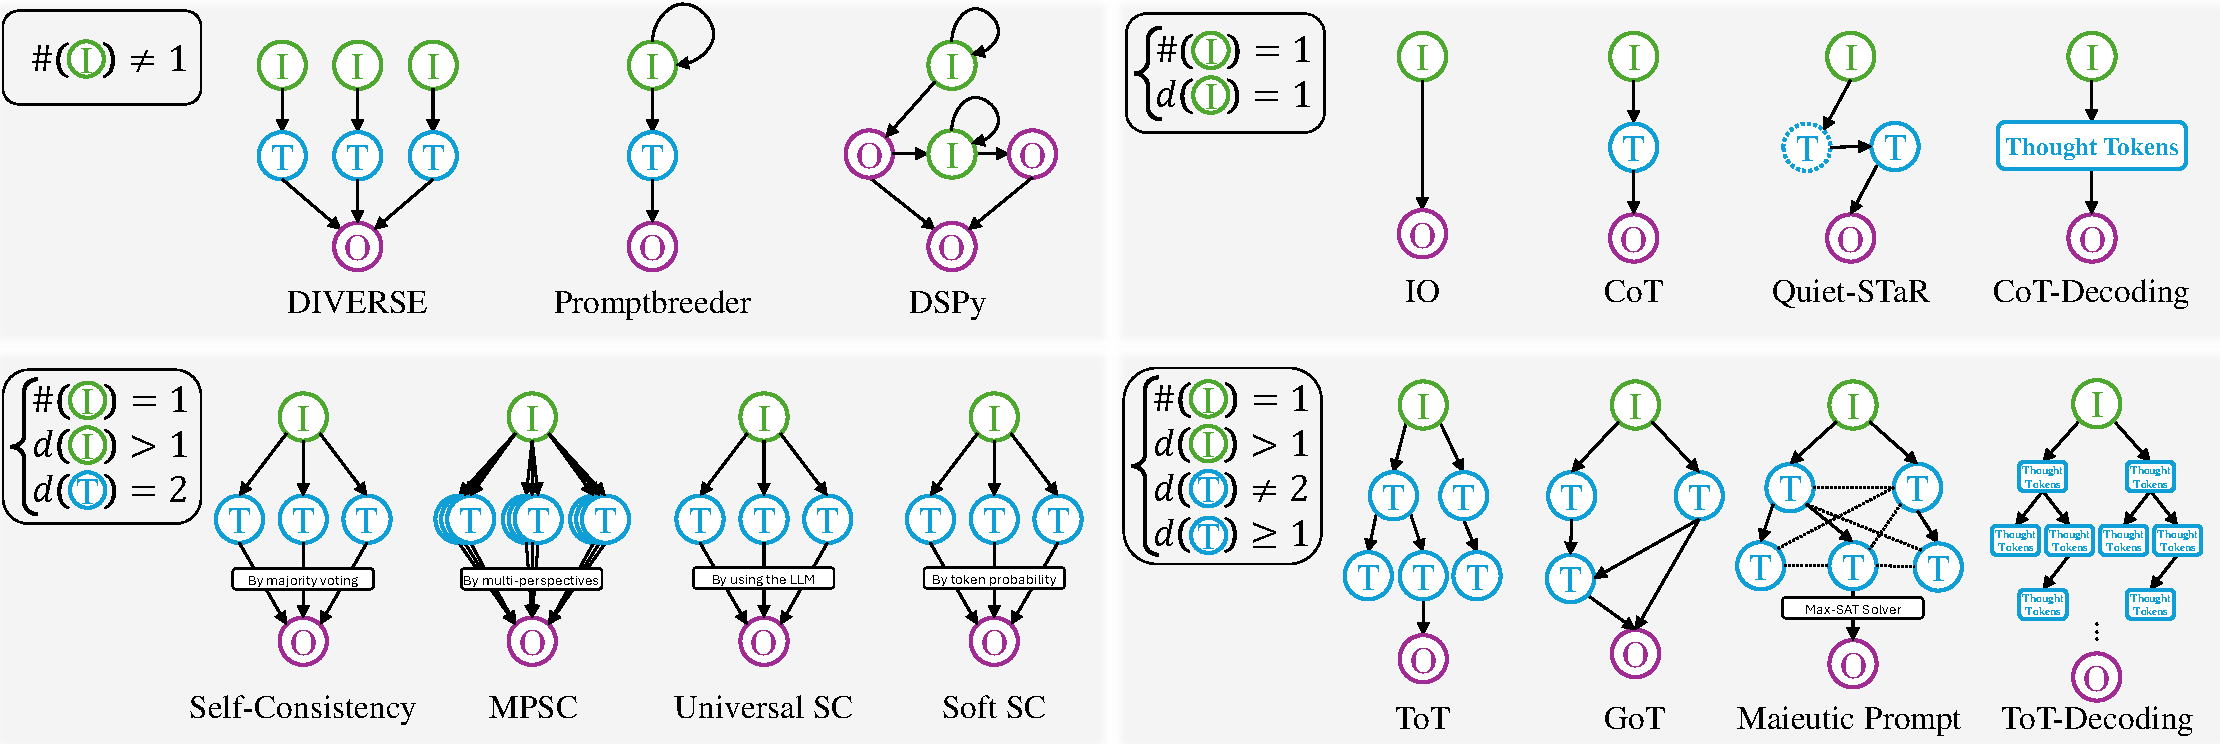
\includegraphics[width=\linewidth]{figures/reason_topo.pdf}
    \caption{Different Reasoning Topologies. \circledColoredChar{darkgreen}{I}/ \circledColoredChar{darkblue}{T}/ \circledColoredChar{darkpurple}{O} indicate input / intermediate thought / output, respectively. $\#(\cdot)$ and $d(\cdot)$ indicate the number and the degree of nodes, respectively.}
    \label{fig:reason_topo}
\end{figure*}

% X-of-Thought 方法简介
A survey~\cite{SurveyXofThought_24_arXiv_ETH} comprehensively examines various X-of-Thought methods, including Chain-of-Thought, Self-Consistency, Tree-of-Thought, and Graph-of-Thought. Here, we briefly introduce these methods. Readers can refer to~\cite{SurveyXofThought_24_arXiv_ETH} for more details. \textbf{Input-Output (IO)} is the most straightforward way to make a model reason. That is, ask a question and get an answer directly. However, due to the lack of intermediate steps, it often fails to solve complex problems. Consequently, the efficient and robust \textbf{Chain-of-Thought (CoT)}~\cite{RealCoT_22_NeuIPS_Google} was proposed, which requires the model to provide intermediate reasoning steps to avoid failures in solving difficult problems. However, this method's limitation is that if there is an error in the reasoning, the final result will also be affected. Subsequently, \textbf{Self-Consistency (SC)}~\cite{SelfConsistency_23_ICLR_Google} was introduced, where a simple majority voting strategy can significantly improve the accuracy of the final answer. Yet, the majority voting strategy is inherently limited in its exploratory capabilities and can only address problems like QA, where there is a fixed answer set, allowing the selection of the most frequent answers from different responses. To address these limitations, \textbf{Tree-of-Thought (ToT)}~\cite{ToT_23_NeuIPS_Princeton} was proposed, which views reasoning as a path linking different thoughts, with each node having multiple successor nodes for thorough local exploration. This method also developed a general scoring system to let the language model evaluate the quality of nodes and decide whether to explore further. \textbf{Graph-of-Thought (GoT)}~\cite{GoT_24_AAAI_ETH} further extended this line of work by providing aggregation among different thought nodes, enhancing the utilization of reasoning chains. \textbf{Maieutic Prompting}~\cite{Maieutic_22_EMNLP_UoWashington}, similar to GoT, attempts to establish entailment relationships between thoughts through rules, then constructs a Max-SAT~\cite{Battiti2009} problem to obtain the best choices.

% 解决问题:只能聚合具有固定Label集合的query
Most X-of-Thought methods require sampling and aggregation of thoughts, often limited to queries with fixed label sets during aggregation. To solve this problem, several works have emerged. \textbf{Multi-Perspective Self-Consistency (MPSC)}~\cite{MPSC_23_arXiv_PKU} targets code generation tasks, evaluating each solution from multiple perspectives (solution, specification, and test case) to select the best one. \textbf{Universal Self-Consistency (Universal SC)}~\cite{UniversalSelfConsistency_23_arXiv_Google} uses LLMs instead of simple answer matching to choose the most selected response, enhancing the stability of the majority voting. \textbf{Soft Self-Consistency (Soft SC)}~\cite{SoftSelfConsistency_24_arXiv_UNCChapel} proposes a more adaptive scoring function, calculating the joint probability of tokens in a response as the scoring function, thus extending the problem scope to soft labels.

% 解决问题:隐含推理和显式推理的矛盾
Additionally, \textbf{Quiet Self-Taught Reasoner (Quiet-STaR)}~\cite{QuietSTaR_24_arXiv_Stanford} addresses the issue mentioned in Section~\ref{sec:hourglass}, where ``although complex reasoning in responses is beneficial for solving intricate problems, they may disrupt model's latent reasoning due to redundant reasoning text, thereby increasing response-level inconsistency.'' Quiet-STaR samples rationales from model's responses and wraps each rationale between special markers, that is, \textless \textbar startofthought\textbar\textgreater\ and \textless \textbar endofthought\textbar\textgreater, to assist next-token reasoning. These rationales are invisible to the user, making latent reasoning explicit and effectively reducing conflicts.

% 推理拓扑拓展到input阶段
However, these lines of work are mostly focused on how to choose the next thought from an input, overlooking the input stage. An input is a combination of a query and a prompt template. While the query remains relatively unchanged, the instructions and demonstrations in the prompt template can be optimized. Several works have explored this area: \textbf{DIVERSE}~\cite{SelfTeach_23_ACL_PKU} pre-constructs various prompt templates to increase prompt diversity. \textbf{Promptbreeder}~\cite{Promptbreeder_23_arXiv_DeepMind} uses genetic algorithms~\cite{genetic_algorithm} to continuously optimize the original prompt template. \textbf{DSPy}~\cite{DSPy_24_ICLR_Stanford} innovatively builds a prompt optimizer, similar to a gradient optimizer in PyTorch. These methods extend reasoning topology to the input stage, demonstrating significant creativity. Boldly, we could construct a reasoning-topology-oriented framework incorporating prompt optimization, which could potentially solve more complex problems.
% TODO: 可以考虑把这个放到 future directions里

% ssc here

% 推理拓扑拓展到decoding阶段
Furthermore, we can extend our approach to the decoding stage. \textbf{CoT Decoding}~\cite{CoT_24_arXiv_Google} incorporates CoT's ideas into the decoding process, attempting to identify CoT-included decoding paths in the natural decoding process. \textbf{ToT Decoding}~\cite{SelfEvaluation_23_NeuIPS_NUS} integrates ToT concepts into decoding, replacing beam search criteria with Self-Evaluation~\cite{TheoryKnowKnow_22_arXiv_Anthropic}, where each token's selection depends on confidence scores $C(\cdot)$, achieving better reasoning, as shown in Eq.~\ref{eq:beam_with_selfeval}, where $\boldsymbol{y}^t$ is the $t$-th token in string $\boldsymbol{y}$.

\begin{equation}
    P(\boldsymbol{y}) = \prod_t P(\boldsymbol{y}^t | \boldsymbol{y}^{1:t-1})C(\boldsymbol{y}^t)
    \label{eq:beam_with_selfeval}
\end{equation}

% Self-Evaluation策略
\textbf{Self-Evaluation Strategy.} The methods discussed in this section typically require searching the thought graph, necessitating evaluators to determine the usefulness of thoughts and whether they merit further exploration. These works generally use three approaches: Majority Voting, selecting the most consistent response among multiple thoughts~\cite{SelfConsistency_23_ICLR_Google}; Rule-based methods, designing specific scoring functions based on the problem, such as error scoring functions in sorting tasks, representing the number of inversions and frequency differences before and after sorting~\cite{GoT_24_AAAI_ETH}; and LLM-based methods, like the scoring function in the Game of 24 task, where LLMs rate the solution's feasibility as ``sure/maybe/impossible''~\cite{ToT_23_NeuIPS_Princeton}.

% Self-Update策略
\textbf{Self-Update Strategy.} For Self-Consistency prompting, the update uses majority voting result. For ToT prompting, the update method uses BFS and DFS strategies to search and select suitable thoughts as output. For GoT prompting, the update method is similar to ToT but includes more extensive search spaces, aggregating different thoughts.

% 方法评价
Despite the innovations, these methods have several limitations~\cite{SurveyXofThought_24_arXiv_ETH}: 1) They often select extremely simple tasks like Game of 24, Sorting, and Keyword Counting for experiments. 2) They incur high reasoning costs. 3) They struggle to adapt to general tasks and deployment.


\subsection{Refining with Responses} \label{sec:refining_with_responses}


\noindent Refining with Responses refers to the process where an LLM first generates multiple responses, then identifies the better responses or self-evaluates its own generated content and corrects errors, and finally refines its output or fine-tunes the model itself to improve response consistency. The following are three common lines of work.

\textbf{Fine-tuning from the collected responses.} This line of work involves ``using self-generated data to fine-tune itself.'' Specifically, they often use LLMs to produce multiple answers, select the better responses from them, and then use these better responses to fine-tune the model, enhancing its reasoning capabilities. For example, Self-Improve proposed by ~\cite{SelfImprove_23_EMNLP_Illinois} uses a majority voting strategy to obtain better outputs, collecting such data to fine-tune the model itself. Similarly, Tian et al.~\cite{SelfImprovement_24_arXiv_Tencent} propose a framework called Self-Improvement, which uses Monte Carlo Tree Search for data synthesis while generating fine-tuning datasets, improving model's reasoning capabilities. This concept is not only effective in the reasoning domain but also finds applications in other fields like the web agent domain. Self-Improved Agents~\cite{WebAgent_24_arXiv_UPenn} improved performance by 31\% using this method. In the preference optimization field, SRPO (Self-Improving Robust Preference Optimization)~\cite{SelfImprove_24_arXiv_Cohere}, and Self-Alignment~\cite{SelfAlignment_23_NeuIPS_CMU} both utilize model-generated preferences to align with human preferences.

\textbf{Learning from mistakes.} This line of work is similar to fine-tuning from the collected responses but focuses on learning from errors and optimizing by avoiding mistakes. This intuitive method naturally improves model performance by avoiding errors. For instance, the LEMA (LEarning from MistAkes) method proposed by~\cite{LearnMistake_24_arXiv_MS} samples multiple reasoning rationales, has GPT-4 annotate and correct errors among them, and uses the corrected rationales to form a new dataset for re-fine-tuning the model. Similarly, Tong et al.~\cite{LearnMistake_24_arXiv_UCSD} propose the Mistake Tuning scheme: it has the model self-rethink and correct its errors based on references, using large amounts of such self-corrected datasets to fine-tune the model.

\textbf{Getting better response with NLI models.} Besides fine-tuning methods, we also demonstrate rule-based optimization techniques using NLI. NLI is a classic task in traditional NLP that can determine the relationship between two statements as entailment / contradiction / neutral. With an NLI model, we can identify the relationships between multiple samples and find better responses. For instance, Agarwal et al.~\cite{NLIConsistency_22_CS224N_Stanford} use a pre-trained NLI model to identify and correct logically inconsistent statements generated by a pre-trained language model. They then convert the entailment and contradiction probabilities of the NLI into a Max-SAT problem~\cite{Battiti2009}, and use a constraint solver~\cite{ignatiev2019rc2} to optimize and obtain more accurate and consistent predictions. Similarly, Mitchell et al.~\cite{ConCoRD_22_EMNLP_Stanford} propose ConCoRD (Consistency Correction through Relation Detection), which further utilizes a pre-trained NLI model to estimate the logical relationships between model predictions, constructs a factor graph representing the prediction probability distribution, and finds the maximum probability prediction result on the factor graph.


\subsection{Multi-Agent Collaboration}  \label{sec:multi_agent}


\noindent The methods in this category generally involve using more than one LLM to collaboratively solve problems, address contradictions, and promote consistency, essentially constituting a generalized form of Self-Feedback. There are numerous papers in the Multi-Agent field; here, we list some typical and novel works that employ Multi-Agent systems for Self-Feedback. For a more comprehensive understanding, refer to the extensive survey on LLM Agents by Wang et al.~\cite{SurveyAgent_24_Frontiers_RUC}.

Multi-Agent Debate~\cite{Debate_23_arXiv_MIT} utilizes multiple peer models that engage in iterative debates, with a fixed number of rounds as the stopping condition. Their experiments show that debates with three or fewer rounds can generally lead to convergence among agents (i.e., LLMs consistently agreeing on the same answer). Xiong et al.~\cite{ModalCollaboration_23_EMNLP_HIT} further propose the FORD (Formal Debate Framework), which introduces a Judge LLM to summarize the agents' statements at the end, also using a fixed number of rounds as the stopping condition. They expand the scope of LLM debates by exploring the effects of debates among models with mismatched capabilities in various scenarios. REFINER~\cite{REFINER_24_EACL_EPFL} trains two models with different roles: a generator for intermediate reasoning steps and a critic for feedback, continuing the iterative dialogue until the correct answer is obtained or the critic has no further feedback. Notably, using the correct answer as a stopping condition has been criticized as unrealistic~\cite{TheoryNoReason_24_ICLR_Google}. 

The Consensus Game proposed by Jacob et al.~\cite{ConsensusGame_24_ICLR_MIT} deviates from the above frameworks by avoiding direct dialogue between LLMs. Instead, different LLMs participate in a game, based on the hypothesis that ``asking a model for answer A to question Q (generative)'' and ``asking a model if A is the answer to Q (discriminative)'' lack consistency~\cite{liang2023uhgeval}. To achieve consistency, they prompt the generator to produce both correct and incorrect answers, then use the discriminator to evaluate its own responses, aiming for the generator and discriminator to reach a consensus (Nash equilibrium). They select the best response based on the degree of consistency.

The significant drawback of this line of work is the high inference cost, as it often requires different LLM instances, potentially consuming multiple times the GPU memory and increasing the inference burden due to the extensive context generated by agents. Additionally, most models need a stopping condition to end the dialogue, and fixed round stopping is inflexible and can reduce performance. There is no current flexible and efficient stopping criterion. However, Multi-Agent systems remain a promising AI direction, and cost issues shouldn't deter exploration. For instance, MACNet (Multi-Agent Collaboration Network)~\cite{MACNet_24_arXiv_THU} uses dozens of agents and various network topologies to collaboratively solve problems. Despite the high costs, such exploration is beneficial for collaborative optimization.


\section{Task: Hallucination Alleviation} \label{sec:hallucination_alleviation}


\noindent Reasoning elevation typically targets QA tasks, while hallucination alleviation is generally aimed at open-ended generation tasks such as story writing and code generation, emphasizing goals like fact enhancement, error reduction, and faithfulness enhancement. This section provides a survey of these directions. We have categorized four significant lines of work, as shown in the lower half of Table~\ref{tab:reason_hall_paradigms}.


\subsection{Refining the Response Iteratively} \label{sec:refining_the_response_iteratively}


\noindent This line of work is similar to Refining with Responses listed in Section~\ref{sec:refining_with_responses}. The difference lies in the focus: Refining with Responses primarily targets QA tasks, where various methods often only need to consider intermediate reasoning steps and the correctness of the final answer. This can be achieved by sampling multiple responses and synthesizing or selecting the better ones. In contrast, hallucination alleviation primarily deals with open-ended tasks such as story generation and code generation. When sampling multiple responses, it is still necessary to meticulously check each response for errors. Therefore, to alleviate hallucinations, it is crucial to iteratively refine and polish a response, eliminating errors. Their comparison is shown in Table~\ref{tab:section_compare}.

\begin{table}[h!]
\centering
\caption{Refining with Responses V.S. Refining the Response Iteratively} \label{tab:section_compare}
\begin{tabular}{p{0.5cm}p{3cm}p{4cm}}
\toprule
            & Section~\ref{sec:refining_with_responses}  & Section~\ref{sec:refining_the_response_iteratively}  \\
\midrule
Name        & Refining with Responses                    & Refining the Response Iteratively                    \\
Train.      & Half needed                                & Few needed                                           \\
Target      & Reasoning Elevation                        & Hallucination Alleviation                            \\
Task        & QA: Math, NLI, etc.                        & Open-Ended: Story, Code, etc.             \\
Steps      & \makecell[l]{1. Sample responses \\ 2. Aggregate them \\ 3. Refine} & \makecell[l]{1. Generate one response \\ 2. Refine it \\ 3. Iterate} \\
\bottomrule
\end{tabular}
\end{table}

This line of work is relatively mature. The most famous include Self-Refine~\cite{SelfRefine_23_NeuIPS_CMU}, Reflexion~\cite{Reflexion_23_NeuIPS_Northeastern}, and Self-Correct~\cite{SelfCorrect_23_ICLR_AI2}. These three frameworks share the basic structure of having the LLM provide textual feedback, which is then used to update the response iteratively until a stopping criterion is met or the maximum iterations is reached, as shown in Algorithm~\ref{alg:refining_the_response_iteratively}.

\begin{algorithm}[h]
\small
\caption{\textsc{Refining the Response Iteratively}}
\label{alg:refining_the_response_iteratively}
\begin{algorithmic}[1]
\REQUIRE Input query $\boldsymbol{x}$, model $\mathcal{M}$, consistency signal generator $\text{SelfEvaluate}(\cdot)$, Self-Update strategy $\text{SelfUpdate}(\cdot)$, stopping criterion $\text{stop}(\cdot)$, max iteration $T$
\STATE $\boldsymbol{y}_0 = \mathcal{M}(\boldsymbol{x})$
\STATE $i \gets 0$
\WHILE {i \textless T \AND \NOT $\text{stop}(\boldsymbol{y}_i)$}
    \STATE $f_i = \text{SelfEvaluate}(\boldsymbol{x}, \boldsymbol{y}_i)$
    \STATE $\boldsymbol{y}_{i+1} = \text{SelfUpdate}(\boldsymbol{x}, \boldsymbol{y}_{0:i}, f_{0:i})$
    \STATE $i \gets i + 1$
\ENDWHILE
\RETURN $\boldsymbol{y}_i$
\end{algorithmic}
\end{algorithm}

We can also formalize the process in Algorithm~\ref{alg:refining_the_response_iteratively} as a conditional language model, as shown in Eq.~\ref{eq:refining_the_response_iteratively}.

\begin{equation}
    P(\boldsymbol{y}|\boldsymbol{x}) = P(\boldsymbol{y}_0|\boldsymbol{x}) \prod_{i=1}^{n} P(\boldsymbol{y}_i|\boldsymbol{y}_{i-1}, \boldsymbol{x}, f_{i-1})
    \label{eq:refining_the_response_iteratively}
\end{equation}

Here, $P(\boldsymbol{y}_0|\boldsymbol{x})$ is a common conditional language model, $n$ denotes the number of iterations, $f_i$ is the Feedback Signal, and $P(\boldsymbol{y}_i|\boldsymbol{y}_{i-1}, \boldsymbol{x}, f_{i-1})$ represents the refinement based on the previous output $\boldsymbol{y}_{i-1}$ and the generated feedback $f_{i-1}$.

Despite following a similar framework, there are differences in specific implementations. Self-Refine~\cite{SelfRefine_23_NeuIPS_CMU} is the most naive implementation, where $\text{SelfEvaluate}(\cdot)$ is entirely performed by the LLM to generate textual feedback. Reflexion~\cite{Reflexion_23_NeuIPS_Northeastern} takes a better approach by viewing the iterative refining process as Verbal Reinforcement Learning, which is reinforcement learning without weight updates. Additionally, they separate feedback into feedback signal generation (e.g., error messages generated after code compilation in code generation tasks) and textual feedback generation (reflecting on error messages), increasing the framework's completeness. However, this approach requires a specific feedback signal design for each task, reducing its generality. Self-Correct~\cite{SelfCorrect_23_ICLR_AI2} uses the same framework but trains a dedicated Corrector model to generate better feedback. This method, however, is still not task-agnostic and significantly reduces the framework's flexibility due to the introduction of training.

The works mentioned above mainly construct frameworks for general tasks, while some focus on specific tasks. For example, Re$^3$~\cite{Re3_23_EMNLP_Berkeley} draws inspiration from human actions in writing long stories and proposes a draft, rewrite, and edit cycle to optimize the LLM's ability to write long stories. PEER~\cite{PEER_23_ICLR_Meta} mimics human collaborative editing by having the LLM iteratively propose editing suggestions to complete Wikipedia text editing. Self-Debug~\cite{SelfDebug_24_ICLR_Google} allows the model to debug its code through execution results and self-written unit test results, gradually refining the code until it is perfected.


\subsection{Mitigating Hallucination while Generating} \label{sec:mitigating_hallucination_while}


\noindent As mentioned earlier, hallucinations often manifest in finer details, such as temporal inaccuracies, date errors, or misattributions of names~\cite{liang2023uhgeval}. Multi-round iterations may overlook these minor errors, prompting some works to propose methods for more granular error editing, mitigating hallucination while generating\footnote{This section incorporates ideas from RAG, yet given its relevance to Self-Feedback, it's delineated as a distinct line of work.}. Currently, this is not yet a relatively mature direction, and there is no unified solution emerging. The following outlines typical approaches in methodology.

M\"undle et al.~\cite{HalluSelfContradictory_24_ICLR_ETH} utilize the phenomenon of Self-Contradiction to eliminate hallucinations\footnote{Demo of Self-Contradiction: \url{https://chatprotect.ai/}}. Specifically, it induces prompts to generate two contradictory sentences and then directs the LLM to resolve the contradictions, retaining the consistent information to generate a coherent response. Subsequent sentences follow a similar approach to produce a complete reply. Clearly, contradictory information is highly likely to be hallucinatory, thus effectively mitigating hallucinations. This method essentially extends Self-Consistency~\cite{SelfConsistency_23_ICLR_Google} into the domain of hallucination.

EVER (REal-Time VErification and Rectification)~\cite{EVER_arXiv_23_UNC} employs a similarly intuitive approach. When generating a sentence, EVER verifies the accuracy of the generated sentence either by the LLM itself or retrieved external information, generating feedback to modify the sentence if there are issues. The modified sentence is then re-appended into the generated text iteratively. Similarly, PURR (Petite Unsupervised Research and Revision)~\cite{PURR_23_arXiv_UCI} and RARR (Retrofit Attribution using Research and Revision)~\cite{RARR_23_ACL_CMU} follow a similar approach as EVER, where the verification stage relies on retrieving external knowledge to provide modification feedback.

In contrast to EVER, FAVA (FAct Vericaton with Augmentation)~\cite{FAVA_24_arXiv_Washington} adopts a more sophisticated approach. It fine-tunes the model to generate tokens that edit its own content, significantly enhancing editing efficiency. Their fine-tuning dataset includes examples like: ``Messi is an \textless entity\textgreater \textless delete \textgreater Argentine \textless /delete \textgreater \textless mark \textgreater Brazilian \textless /mark \textgreater \textless /entity \textgreater soccer player.'' Special tokens enclosed in angle brackets are also trained to be generated, effectively eliminating hallucinations through rendering. The major advantage of this method lies in granting the LLM maximum autonomy to make mistakes and subsequently correct them freely. Moreover, this approach bears resemblance to Quiet-STaR~\cite{QuietSTaR_24_arXiv_Stanford} mentioned in Section~\ref{sec:reasoning_topologically}, where both utilize special tokens to represent non-essential cognitive processes.


\subsection{Decoding Truthfully} \label{sec:decoding_truthfully}


\noindent The concepts of ``Refining the response iteratively'' and ``Mitigating hallucination while generating'' primarily aim to enhance response consistency. Conversely, Decoding Truthfully focuses predominantly on decoding consistency. In recent years, several studies have discovered that methods such as greedy decoding and sample decoding alone constrain LLMs from accurately expressing crucial information in natural language form within latent layers. Consequently, more complex and rational decoding strategies have been designed to elevate the reliability and accuracy of model's responses.

Li et al.~\cite{CD_22_arXiv_Stanford} pioneered the Contrastive Decoding strategy, where during the next token prediction, the optimal token probability is selected by contrasting the token probability distributions derived from expert and amateur models, as shown in Eq.~\ref{equ:ContrastiveDecode}. This method excels in mitigating biases or preferences inherent in large-scale models, favoring tokens with higher probabilities in expert models and lower probabilities in amateur models.

\begin{equation}
\label{equ:ContrastiveDecode}
\boldsymbol{y}^t \sim \operatorname{softmax}\left(\log \frac{P_{\mathrm{EXP}}\left(\boldsymbol{y}^t \mid \boldsymbol{y}^{0:t-1}\right)}{P_{\mathrm{AMA}}\left(\boldsymbol{y}^t \mid \boldsymbol{y}^{0:t-1}\right)}\right)
\end{equation}

Following this pioneering work, researchers have explored various approaches for logit adjustment and contrastive decoding. Chuang et al.~\cite{DoLa_24_ICLR_MIT} observed significant differences in token probability distributions across different layers of the model and introduced DoLa to incorporate information from previous layers, enhancing early-stage cognitive reasoning and pre-answer consistency, termed Decoding Consistency.

Unlike DoLa, SED~\cite{SED_24_arXiv_FDU} and DIVER ~\cite{DIVER_24_arXiv_IA} focus on detecting and addressing discrepancies caused by differences in tokens at certain positions, termed Chaotic Points. Methods for detecting chaotic points include comparing the ratio of maximum to second-maximum token probabilities and ensuring the number of candidate tokens exceeds one, as shown in Eqs.~\ref{equ:chaotic_ratio} and ~\ref{equ:chaotic_base}, where $\delta_r$ is a probability threshold, $\gamma$ is a predefined coefficient, and $\mathcal{V}$ denotes the vocabulary. By assessing generated content against previously generated segments and potential tokens from chaotic points, scores such as information gain, weighted uncertainty, and weighted confidence help identify the most suitable token.

\begin{equation}
\label{equ:chaotic_ratio}
\mathbb{I}_1=\mathbb{I}\left(P_{\text {gen}}\right)=\left(\frac{P_{\text {second }}}{\boldsymbol{p}_{\text {max }}} \geq \delta_r\right)
\end{equation}

\begin{equation}\label{equ:chaotic_base}
\begin{aligned}
\tau &= \gamma \max_{w \in \mathcal{V}} P\left( w \mid \boldsymbol{y}^{0:t-1}\right) \\
\mathbb{I}_2 &= \left( \left| \left\{ \boldsymbol{y}^t \in \mathcal{V} \mid P\left( \boldsymbol{y}^t \mid \boldsymbol{y}^{0:t-1}\right) \geq \tau \right\} \right| > 1 \right)
\end{aligned}
\end{equation}


Those methodologies primarily apply to closed-book generation tasks. For open-book generation tasks, current research focuses on leveraging external references to guide decoding. CAD~\cite{ContextAwareD_23_arXiv_Washington} and ECAD~\cite{ContextDecode_24_arXiv_Edin} (named ECAD in this review) incorporate contextually relevant or irrelevant knowledge snippets into model inputs, intervening in the decoding process through contrastive decoding strategies to bridge the information gap between useful and non-useful information. To further exploit valuable information from references, FastMem~\cite{FastMem_24_arXiv_KUL} fine-tunes the final layer of LLMs to quickly memorize reference texts during inference, highlighting differences in decoding with and without references.

In summary, these studies identify internal inconsistency phenomena or instability in responses to guide LLMs' probability distributions during decoding.


\subsection{Activating Truthfulness} \label{sec:activate_truth}


\noindent  Activating Truthfulness focuses on enhancing consistency in latent layers. Its core methods involve boosting attention heads and states that represent ``truthfulness'' within latent layers, or refining latent layers through fine-tuning, aiming to improve the model's internal consistency.

The exploration of latent truthfulness began with CCS (Contrast-Consistent Search) proposed by Burns et al.~\cite{CCS_23_ICLR_UCB}. CCS investigates methods for mining knowledge embedded in latent layers by training a small classification head on Transformer latent layers. This method effectively activates model truthfulness, surpassing conventional inference methods.

Inspired by CCS, scholars from Harvard University developed the Inference-Time Intervention (ITI) technique~\cite{ITI_23_NeuIPS_Harvard}. This technique involves two main steps: 1. Probe analysis: Using probe technology\footnote{A probe is a small classifier where the input is latent states and the output is labels corresponding to a test task. In ITI, this test task is TruthfulQA~\cite{lin-etal-2022-truthfulqa}, where a subset of test tasks trains the probe to identify attention heads associated with higher truthfulness (higher classification accuracy).} to identify attention heads in the model related to truthfulness. 2. Inference-time intervention: Adjusting selected attention heads during the model's answer generation process by increasing their weights. This guides the model towards more truthful reasoning paths. However, ITI has limitations in training probes using the last token's latent layer state at the end of a question-answer pair. This approach lacks features and turns the problem into discerning truthfulness rather than generating truthful content (generative). Addressing these issues, TrFr~\cite{TrFr_24_AAAI_BUAA} proposed the use of multi-dimensional orthogonal probes, effectively extracting features from both truthful and non-truthful texts to better identify effective attention heads. TruthX~\cite{TruthX_24_ACL_ICT} explored a more efficient intervention strategy. It targets not only attention heads but also latent states in the forward feedback layer. Mapping these states separately using truthful and semantic encoders significantly reduces the impact on the language model's overall performance while enhancing representations of truthfulness.

% TODO 低优先级 字典学习和sae需要再细读下
Besides improving truthfulness, what other characteristics do latent layers possess? Recently, more work has begun to explore various features within latent layers. This not only demystifies model black boxes but also offers potential methods to mitigate hallucination issues. For example, Wu et al.~\cite{RetrievalHead_24_arXiv_PKU} discovered that some attention heads focus more on long-context retrieval capabilities (strong copy-paste needle abilities). In tests like Needle-in-a-Haystack, blocking these attention heads results in performance dropping from 94.7\% to 63.6\%. Can enhancing model retrieval heads reduce hallucinations in long contexts? This is a question worth exploring. For another example, teams from Anthropic also used dictionary learning to discover monosemanticity within LLMs~\cite{templeton2024scaling}, such as ``Golden Gate Bridge.'' Activating states corresponding to the ``Golden Gate Bridge'' in latent layers leads the model to consider itself as the bridge. OpenAI also proposed Sparse Autoencoder (SAE)~\cite{gao2024scaling} to automatically identify latent features within language models.

% TODO: 可添加到future direction里,拟人性注意力头
If feature exploration were more accessible, could we identifying ``human-likeness'' features that can prevent models from mistakenly perceiving themselves as human, thus reducing hallucinations related to cognitive errors? Exploring latent features in language models to subsequently reduce hallucinations from a white-box perspective is a promising direction. However, the main challenge lies in the inefficiency of probe technology, dictionary learning, SAE, and similar methods, which require training many classifiers to effectively extract latent features from models.

% TODO 低优先级 列一个表格,比较 inference-time activating truthfulness 和 training-time activating truthfulness
In addtion to implicit feature mining methods, Activating Truthfulness also includes truthfulness-oriented fine-tuning methods that essentially explore consistency within latent states. For instance, Tian et al.~\cite{FactualFT_23_arXiv_Stanford} proposed sampling multiple responses from an LLM and using Self-Evaluation to identify more factual responses. Collecting these QA pairs and retraining the original LLM aligns with the fine-tuning approach mentioned in Section~\ref{sec:refining_with_responses}, though it is not the primary focus of this section.


\section{Task: Others} \label{sec:other_tasks}


\noindent Apart from reasoning elevation and hallucination alleviation, several lines of work follow the Self-Feedback framework, although their objectives are not to improve the model's internal consistency. Examples include knowledge distillation, preference learning, and data augmentation. For the sake of completeness in this survey, this section briefly summarizes these other works adhering to the Self-Feedback framework.


\subsection{Preference Learning} \label{subsec:PL}



\noindent Currently, the responses of LLMs in specific domains sometimes fail to satisfy users, even violating human values, social ethics, and morals. The goal of Preference Learning is to enable LLMs to better follow human instructions and output responses that meet human expectations. Most of the work around this task can be broadly covered by the Self-Feedback framework. Specifically, the model generates initial responses during the Self-Evaluation process and then performs Self-Update based on the Feedback Signal. Here, the Feedback Signal mainly refers to the reward information given by a reward model $\mathcal{R}$, which is trained through preference feedback. Preference feedback involves comparing and ranking different responses to the same question in terms of helpfulness, harmlessness, and honesty. The Self-Update here primarily refers to broadly updating the model $\mathcal{M}$, including methods like supervised fine-tuning and reinforcement learning (such as PPO~\cite{PPO_17_arXiv_OpenAI}, DPO~\cite{DPO_23_NIPS_Stanford}).

There are three main ways to obtain preference feedback. The first is through human feedback, as seen in works like OASST~\cite{OASST_23_NIPS_XX} and BeaverTails~\cite{BeaverTails_23_NIPS_PKU}, which include human-annotated data from multiple annotators. The second method involves feedback generated by models~\cite{ConstitutionalAI_22_arXiv_anthropic,SALMON_24_ICLR_IBM,RLAIF_22_arXiv_anthropic}, offering lower annotation costs and faster iterative feedback efficiency compared to human feedback. The third type of feedback is derived from inductive bias. For instance, the SHP dataset mentioned in~\cite{DataDifficult_22_PMLR_UoW} considers upvotes and downvotes to differentiate between good and bad responses. Another example is ALMoST~\cite{ALMoST_23_arXiv_NAVER}, which proposes some prior rules, such as larger parameter models generally performing better, and more prompt context examples yielding higher quality responses. These rules are used to rank response quality across different models as preference feedback.

Based on preference feedback, we can train a reward model to output Feedback Signals. There are two common types of reward models. One is the Reward Model proposed in InstructGPT~\cite{InstructGPT}, with the loss function as shown in Eq.~\ref{equ:reward_model}. Here, $r_\theta(\boldsymbol{x}, \boldsymbol{y})$ represents the output of the Reward Model, and response $\boldsymbol{y}_w$ is ranked higher than $\boldsymbol{y}_l$. However, this method's downside is that the overall score distribution for high-quality and low-quality responses is similar, making it difficult to effectively distinguish between different responses to different questions. To address this, Xu et al.~\cite{SelfCritique_24_arXiv_Zhipu} proposed an evaluation model that directly scores QA pairs.

\begin{equation}\label{equ:reward_model}
\begin{aligned}
z &= \sigma\left(r_\theta\left(\boldsymbol{x}, \boldsymbol{y}_w\right) - r_\theta\left(\boldsymbol{x}, \boldsymbol{y}_l\right)\right) \\
\operatorname{loss}(\theta) &= -\frac{1}{\binom{k}{2}} E_{\left(\boldsymbol{x}, \boldsymbol{y}_w, \boldsymbol{y}_l\right) \sim D}\left[\log \left(z\right)\right]
\end{aligned}
\end{equation}


% 上面提到的工作在Self-Update阶段都是重新推理,与其不同,RLAIF~\cite{RLAIF_22_arXiv_anthropic}使用AI反馈进行强化学习,其中教师模型对学生模型的输出进行排名,得到一个数据集,以此为Feedback Signal,并在Self-Update阶段使用得到的数据集来训练学生模型。
% 类似地,ReST算法~\cite{ReST_23_arXiv_Google}利用学习得到的奖励模型对学生产生的多个输出进行排名,构建数据集。


\subsection{LLM-Based Knowledge Distillation} \label{subsec:KD}


\noindent Small-parameter LLMs have faster inference and training speeds, but their reasoning capabilities are inferior to those of large-parameter LLMs. LLM-based knowledge distillation methods aim to transfer advanced capabilities from proprietary LLMs (such as GPT-4) to small-parameter open-source models (such as LLaMA and Mistral)~\cite{SurveyKD_24_arXiv_HKU}. These two models can be referred to as the ``teacher model'' and the ``student model'' respectively, with the teacher model guiding the student model to enhance its capabilities, fitting the generalized Self-Feedback framework proposed in this paper. During the Self-Evaluation, the student model generates answers, which are then assessed by the teacher model. In the Self-Update, the student model uses the evaluation signal to update itself or its answers.

This signal can be in the form of statistical metrics, such as MiniLLM~\cite{MiniLLM_24_ICLR_THU} calculating the reverse Kullback-Leibler (KL) divergence of the probability distributions output by the student and teacher models; or GKD~\cite{GKD_24_ICLR_Google} computing metrics like forward KL divergence, reverse KL divergence, and generalized JSD. The signal can also be in the form of natural language feedback, such as Selfee~\cite{Selfee_23_blog} utilizing ChatGPT as the teacher to provide textual feedback on the outputs of the student model; or in PERsD~\cite{PERsD_23_EMNLP_NTU}, where the teacher executes the code generated by the student model and provides specific suggestions based on errors.

% FIGA~\cite{FIGA_24_ICLR_RUC}中教师根据学生的响应和golden response进行对比并据此反馈修改意见。
% 另外,还有研究者使用教师模型对学生模型生成的token概率分布进行评价反馈,然后学生模型结合反馈信息进行梯度更新。如

When the teacher and student models are the same LLM, this leads to Self-Knowledge Distillation (Self-KD). In Self-KD, the model iteratively updates its capabilities using the knowledge it gradually accumulates during training, falling under the narrow Self-Feedback paradigm. For example, the goal of Impossible distillation~\cite{ImposDistill_23_arXiv_UoW} is to obtain a Stronger Paraphraser. In the Self-knowledge distillation process, it evaluates its paraphrase results from perspectives such as semantics, format, and diversity, and further refines high-quality data to fine-tune itself accordingly.

% Hahn et al.~\cite{SelfKnowledge_19_RANLP_Handong}观察到在语义空间中相近的token应该有相似的logit值,于是设计在训练过程中获取并利用token的嵌入向量修正对应token的目标概率,然后利用这个修正后的概率计算损失函数并进行梯度更新。
% 类似地,~\cite{TFKD_20_CVPR_NUS}采用了Label Smoothing Regularization的方法将目标标签转化为软概率标签。~\cite{PSKD_21_ICCV_LG}用上一轮训练得到的checkpoint推理得到一个概率分布,将这个分布和目标标签加权得到软概率标签。


\subsection{Data Augmentation}


\noindent Data Augmentation aims to construct and filter high-quality datasets using LLMs. It is somewhat similar to the methods in Sections \ref{subsec:PL} and \ref{subsec:KD} that combine Feedback information to create datasets, but there are slight differences in focus and specific forms. The latter focuses on the model's capabilities, using datasets during the Self-Update stage for model fine-tuning, with most methods falling under narrow Self-Feedback. In contrast, Data Augmentation focuses on the dataset itself, updating the model's responses during the Self-Update stage to further refine the dataset, with most methods falling under generalized Self-Feedback.

Self-instruct~\cite{SelfInstruct_23_ACL_Washington} is a typical example, where the LLM generates new task instructions during the Self-Evaluation stage and generates input-output instances based on the new instructions. It calculates the ROUGE-L metric between the new instructions and existing instructions as the Feedback signal. Finally, during the Self-Update stage, it filters and screens the newly generated set of instructions.

Currently, methods applying LLMs to Data Augmentation and Synthetic Data Generation mainly focus on the prompt engineering layer. In other words, Self-Evaluation only involves responses. Many studies have shown that LLM responses are highly sensitive to prompt variations~\cite{PromptSensitive_23_arXiv_UoW,yu2024xfinder}. Therefore, the main bottleneck in this task is: how to design better prompts and how to deeply explore the relationship between decoding, latent space, and data quality.


% \subsection{}
% 持续学习
% TODO:再列举新方向有必要,但优先级低


\section{Evaluation} \label{sec:evaluation}


\noindent Evaluation helps identify the strengths and weaknesses of different models and methods. This section lists evaluation methods and benchmarks for Internal Consistency and Self-Feedback. These evaluations mainly cover two types of abilities: meta ability, such as model's uncertainty, consistency, and feedback ability; and common ability, which pertains to solving real-world problems, such as reasoning QA tasks and code generation tasks. Meta evaluation helps us identify which LLMs are more promising for solving complex problems, while common evaluation helps us understand which Self-Feedback methods can better solve problems for a given LLM.


\subsection{Meta Evaluation}


\noindent We summarize five meta evaluation methods. These methods can generally be categorized into metric-based and benchmark-based paradigms. The former constructs mathematical formulas or metrics to directly calculate the performance of a particular aspect; the latter uses QA datasets to empirically measure performance. We summarize benchmark-based meta evaluations in Table~\ref{tab:meta_eval}.

\begin{table}[h!]
\centering
\caption{Meta Evaluation Benchmarks} \label{tab:meta_eval}
\begin{tabular}{lll}
\toprule
\textbf{Type} & \textbf{Benchmark} & \textbf{Organization} \\
\midrule
Uncertainty & LLM-Uncertainty-Bench~\cite{UncertaintyBench_24_arXiv_Tencent} & Tencent \\
Uncertainty & UBench~\cite{UBench_24_arXiv_Nankai} & Nankai \\
Consistency & ConsisEval~\cite{ConsisEval_24_arXiv_PKU} & PKU \\
Consistency & PopQA-TP~\cite{PopQA_23_GEM_IBM} & IBM \\
Consistency & ParaRel~\cite{ParaRel_21_TACL_BarIlan} & BIU \\
Consistency & BMLAMA~\cite{CrossLingualConsistency_23_EMNLP_UoGroningen} & RUG \\
Consistency & BECEL~\cite{BECEL_22_Coling_Oxford} & Oxford \\
Critique Ability & CriticBench~\cite{CriticBench_24_arXiv_THU} & THU \\
Self-Knowledge & SelfAware~\cite{TheoryKnowUnknown_23_ACL_Fudan} & Fudan \\
Self-Knowledge & Idk(I don't know)~\cite{TheoryKnowUnknown_24_arxiv_Fudan} & Fudan \\
Self-Knowledge &  Self-Knowledge Evaluation~\cite{EvalSelf_24_arXiv_THU} & THU \\
\bottomrule
\end{tabular}
\end{table}


\textbf{Metric-Based Uncertainty Evaluation.} As mentioned in Section~\ref{sec:uncertainty}, uncertainty estimation involves assessing the uncertainty of a model's specific response. Uncertainty evaluation, on the other hand, measures the overall uncertainty of a model. Key metrics for evaluating model uncertainty include: Expected Calibration Error (ECE), which assesses the expected difference between model confidence and accuracy; Maximal Calibration Error (MCE), which indicates the maximum deviation between model accuracy and confidence; and Brier Score (BS), which is used to assess how closely the model’s predicted probabilities align with the true class probabilities~\cite{SurveyUncertainty_23_arXiv_Nankai}.

\textbf{Benchmark-Based Uncertainty Evaluation.} LLM-Uncertainty-Bench~\cite{UncertaintyBench_24_arXiv_Tencent} extracts five test tasks (including question answering, reading comprehension, commonsense inference, dialogue response selection, and document summarization) from common benchmark datasets and uses conformal prediction techniques to construct benchmarks. UBench~\cite{UBench_24_arXiv_Nankai} also extracts data from other datasets, totaling 3978 multiple-choice questions covering knowledge, language, understanding, and reasoning abilities. UBench evaluates individual data items by having models textually express uncertainty scores.

\textbf{Benchmark-Based Consistency Evaluation.} This line of work centers on assessing whether a model delivers consistent responses to queries that are semantically equivalent but phrased differently. The key focus is on developing a variety of synonymous queries to test the model's reliability. For instance, the ConsisEval Benchmark~\cite{ConsisEval_24_arXiv_PKU} creates simpler synonymous queries for each question. PopQA-TP~\cite{PopQA_23_GEM_IBM} and ParaRel~\cite{ParaRel_21_TACL_BarIlan} construct synonymous queries through rephrasing. BMLAMA~\cite{CrossLingualConsistency_23_EMNLP_UoGroningen} focuses on multilingual consistency, constructing a parallel corpus of queries. BECEL~\cite{BECEL_22_Coling_Oxford} draws inspiration from behavioral consistency, considering higher-order consistency in model responses by creating semantic consistency data, negational consistency data, symmetric consistency data, etc. Notably, most studies have found that models generally exhibit low consistency.

\textbf{Benchmark-Based Critique Abilitiy Evaluation.} Lin et al.~\cite{CriticBench_24_arXiv_THU} collect a large number of QA pairs from 15 datasets across mathematical, commonsense, symbolic, coding, and algorithmic fields, creating CriticBench through model generation and human annotation. It can be used to evaluate the ability of LLMs to generate critiques, an important aspect of the Self-Feedback framework.

\textbf{Benchmark-Based Self-Knowledge Evaluation.} Self-Knowledge refers to the LLM's understanding and recognition of its own abilities, limitations, and the content it creates. Yin et al.~\cite{TheoryKnowUnknown_23_ACL_Fudan} and Cheng et al.~\cite{TheoryKnowUnknown_24_arxiv_Fudan} construct sets of unanswerable questions to explore the question ``Do large language models know what they do not know?'' Tan et al.~\cite{EvalSelf_24_arXiv_THU} investigate ``Does the model truly understand the questions and solutions it creates?'' These studies generally yield negative empirical results, indicating that models have weak Self-Knowledge.


\subsection{Common Evaluation}


\noindent In most works utilizing the Self-Feedback framework, they do not conduct meta evaluations in experiments but rather assess the model's ability to solve real-world problems, such as solving math problems, code generation, and summarizing articles. Here, we classify and summarize the popular benchmarks based on the focus of the evaluation tasks\footnote{We may see the same benchmark categorized differently in different sources, highlighting the difficulty in achieving fully orthogonal classifications. For example, a dataset evaluating linguistic understanding ability may also involve reasoning tasks. Here, we classify each dataset based on its primary focus.}, as shown in Table~\ref{tab:benchmarks}. There are two types of reasoning: Knowledge reasoning focuses on the LLM's ability to solve problems using its parameterized knowledge, while Logic reasoning focuses on complex logical reasoning based on prompts. Linguistic understanding focuses on the LLM's analysis of language meaning. Code generating and Math Solving respectively test the LLM's ability to write code and solve math problems.


\begin{table}[h!]
\centering
\begin{threeparttable}

\caption{Common Evaluation Benchmarks}
\label{tab:benchmarks}


\begin{tabular}{lll}
\toprule
\textbf{Type} & \textbf{Benchmark} & \textbf{Organization} \\
\midrule
Knowledge reasoning                          & C-Eval~\cite{CEval}                          & SJTU                                    \\
Knowledge reasoning                          & MMLU~\cite{hendrycks2021measuring,MMLU2}     & UCB                                  \\
Logic reasoning                              & BBH~\cite{Bench_BBH}                         & Google                                   \\
Logic reasoning                              & ARC~\cite{ARC_c}                             & AI2                                  \\
Linguistic understanding                     & WiC~\cite{bench_WiC}                         & Cambridge                                   \\
Code generating                              & HumanEval~\cite{HumanEval}                   & N/A                                  \\
Math Solving                                        & MATH~\cite{bench_math}                       & UCB                                   \\
Math Solving    & GSM8K~\cite{cobbe2021training}               & OpenAI                                  \\ 
\bottomrule
\end{tabular}

% \begin{tablenotes}
% \footnotesize
% \item \textit{Note}: Citation counts are as of July 10, 2024
% \end{tablenotes}

\end{threeparttable}

\end{table}

Currently, these Benchmark evaluation formats mainly include multiple-choice questions and text generation, each with its own advantages and disadvantages. For multiple-choice questions, evaluators can accurately calculate metrics such as accuracy by extracting answer text from the response or comparing the probabilities of different option tokens during LLM decoding. However, many researchers pointed out the drawbacks of this method, namely that LLMs tend to choose the first option, leading to poor self-consistency and not reflecting the LLM's true ability~\cite{FTEvsTOE_24_arxiv_LMU,wang2024answersreviewingrationalitymultiple}. Text generation tasks, such as math problems and code generation, mitigate the shortcomings of multiple-choice questions by allowing the LLM to perform freely, better reflecting the model's true ability. However, this evaluation method struggles to precisely quantify the gap between generated text and reference answers in dimensions such as syntax and semantics. It is evident that current Benchmarks for common evaluation are still far from accurately measuring the true capabilities of LLMs and have many areas for improvement.


\section{Does Self-Feedback Really Work?}  \label{sec:does_it_work}


\subsection{Conflicting Viewpoints} \label{sec:conflict}


\noindent All methods in this survey suggesting that models can generate proper Feedback Signals to optimize themselves. However, with the emergence of a series of works prefixed with ``Self-'', questions about their feasibility have also arisen: Can models really self-correct, self refine, etc.?

Jiang et al.~\cite{SelfIncorrect_24_arXiv_JHU} propose the SELF-[IN]CORRECT hypothesis. It experimentally verifies in the context of QA tasks that the ``accuracy of generating initial answers (generative)'' is higher than the ``accuracy of judging the correctness of its own generated answers (discriminative)''. This indicates models struggle to assess their own content accurately. They argue that models form a definitive belief about a particular choice during generation, which refutes works like Refining with Responses and Refining the Response Iteratively. However, this work can only refute studies in the domain of QA tasks. Moreover, the model's discriminative ability is not always greater than its generative ability, so it cannot be concluded that various methods cannot achieve self-correction.

Stechly et al.~\cite{GPT4Doesnt_23_NeurIPS_ASU} and Valmeekam et al.~\cite{CanSelfCritique_23_NeurIPS_ASU} used similar strategies to test whether GPT-4 possesses the Self-Feedback capability. Stechly et al.~\cite{GPT4Doesnt_23_NeurIPS_ASU} used the Graph Coloring task to test and found that in work similar to Refining the Response Iteratively, GPT-4 almost always fails to verify the correctness of its own solutions but acknowledges methods like Self-Consistency, which suggest that the model can select appropriate solutions from multiple options. In contrast, Valmeekam et al.~\cite{CanSelfCritique_23_NeurIPS_ASU} tested similar strategies in the task planning domain, refuting the feasibility of both Refining the Response Iteratively and Multi-Agent Collaboration. Both Stechly et al.~\cite{GPT4Doesnt_23_NeurIPS_ASU} and Valmeekam et al.~\cite{CanSelfCritique_23_NeurIPS_ASU} believe that models have difficulty making correct judgments about their own outputs.

The above criticisms often focus on narrow Feedback Signals. In comparison, the criticisms from Huang et al.~\cite{TheoryNoReason_24_ICLR_Google} are more reasonable. Huang et al.~\cite{TheoryNoReason_24_ICLR_Google} specifically refute the effectiveness of three works (Reflexion~\cite{Reflexion_23_NeuIPS_Northeastern}, Multi-Agent Debate~\cite{Debate_23_arXiv_MIT}, and Self-Refine~\cite{SelfRefine_23_NeuIPS_CMU}) through reasonable comparisons and comprehensive experiments. Reflexion relies on external golden truth as a stopping condition for iterative refining during self-correction, which is an unreasonable setup---if there is already a golden truth, there is no need for predictions. For Multi-Agent Debate, the authors' experiments found that this method is significantly inferior to the Self-Consistency strategy and consumes substantial memory. For Self-Refine, the authors found that the prompts used for initial results and refining were unfair, and they generated a fairer prompt that produced better responses in one go.

Due to the different characteristics of various works, Kamoi et al.~\cite{SurveySelfCorrection_24_arXiv_PSU} provide a more comprehensive analysis by constructing a clear classification method and systematically comparing the strengths and weaknesses of each types of work. They suggest that the ability to self-correct should be discussed according to the specific task. For example, for tasks with decomposable responses\footnote{For instance, in the question ``Who are some politicians who were born in Boston?'', the feedback generation can be decomposed into easier sub-tasks of verifying each answer.} or verifiable tasks\footnote{For example, in the Game of 24, a task to find arithmetic operations to obtain 24 using four provided integers, generating a feasible solution might be harder than verification.}, it is feasible for the model to optimize itself.

Although the survey~\cite{SurveySelfCorrection_24_arXiv_PSU} provides more meaningful viewpoints through classified discussions, it complicates the field, making it difficult to form a systematic framework. Benefiting from the perspective of Internal Consistency and the clear boundary discussions in Section~\ref{sec:out_of_scope}, we conduct a more meaningful discussion on the proposed Self-Feedback framework: 

\begin{enumerate}
    \item Does Self-Feedback improve Internal Consistency?
    \item Does Internal Consistency mean correctness?
\end{enumerate}


\subsection{Does Self-Feedback Improve Internal Consistency?}


\noindent For this question, the different lines of work proposed in this paper actually provide affirmative answers from various perspectives. For example,

\begin{itemize}
    \item Self-Consistency~\cite{SelfConsistency_23_ICLR_Google} (Reasoning Topologically) improves response consistency by finding the majority vote from the sampling set. 
    \item Self-Improve~\cite{SelfImprove_23_EMNLP_Illinois} (Refining with Responses) also uses majority voting to find better responses from the sampling set and then fine-tunes the model itself, improving consistency from the parameter level.
    \item Multi-Agent Debate~\cite{Debate_23_arXiv_MIT} (Multi-Agent Collaboration) involves multiple models participating in answering questions simultaneously, which is essentially a generalized way to obtain consistent responses. 
    \item Self-Refine~\cite{SelfRefine_23_NeuIPS_CMU} (Refining the Response Iteratively) iteratively optimizes its responses, which is an implicit way to achieve high-consistency responses. 
    \item Self-Contradict~\cite{HalluSelfContradictory_24_ICLR_ETH} (Mitigating Hallucination while Generating) eliminates self-contradictory content in its responses, naturally improving consistency. 
    \item DoLa~\cite{DoLa_24_ICLR_MIT} (Decoding Truthfully) compares the probability distributions across different layers of the model's latent layers and reduces their discrepancies through comparison, thereby improving the model's consistency.
    \item ITI~\cite{ITI_23_NeuIPS_Harvard} (Activating Truthfulness) implicitly optimizes the model's Internal Consistency by identifying attention heads that prefer factual information.
\end{itemize}


\subsection{Does Internal Consistency Mean Correctness?}


\noindent To answer this question, let's revisit the relationship between world knowledge, corpus, and language models, as shown in Fig.~\ref{fig:knowledge}. World knowledge is the consensual (correct) knowledge we humans possess. The training corpus used for models is a true subset of world knowledge, containing the vast majority of correct knowledge and a small portion of uncleanable erroneous knowledge. Additionally, the knowledge embedded in the corpus is deterministic, where each statement in the corpus has a probability of 100\%. Language models, by fitting the corpus, acquire higher-order probabilistic representations of this knowledge, and the probabilistic nature makes the learned knowledge vague and non-deterministic, as illustrated by the shaded areas in Fig.~\ref{fig:knowledge}. Vagueness (or hallucination) is an important characteristic of language models. It enables the generation of novel and creative expressions outside the training corpus distribution. However, from a reliability perspective, vagueness is a disaster. Vagueness means that answers to the same question are uncertain, making the model's expressions inconsistent.


\begin{figure}[h!]
    \centering
    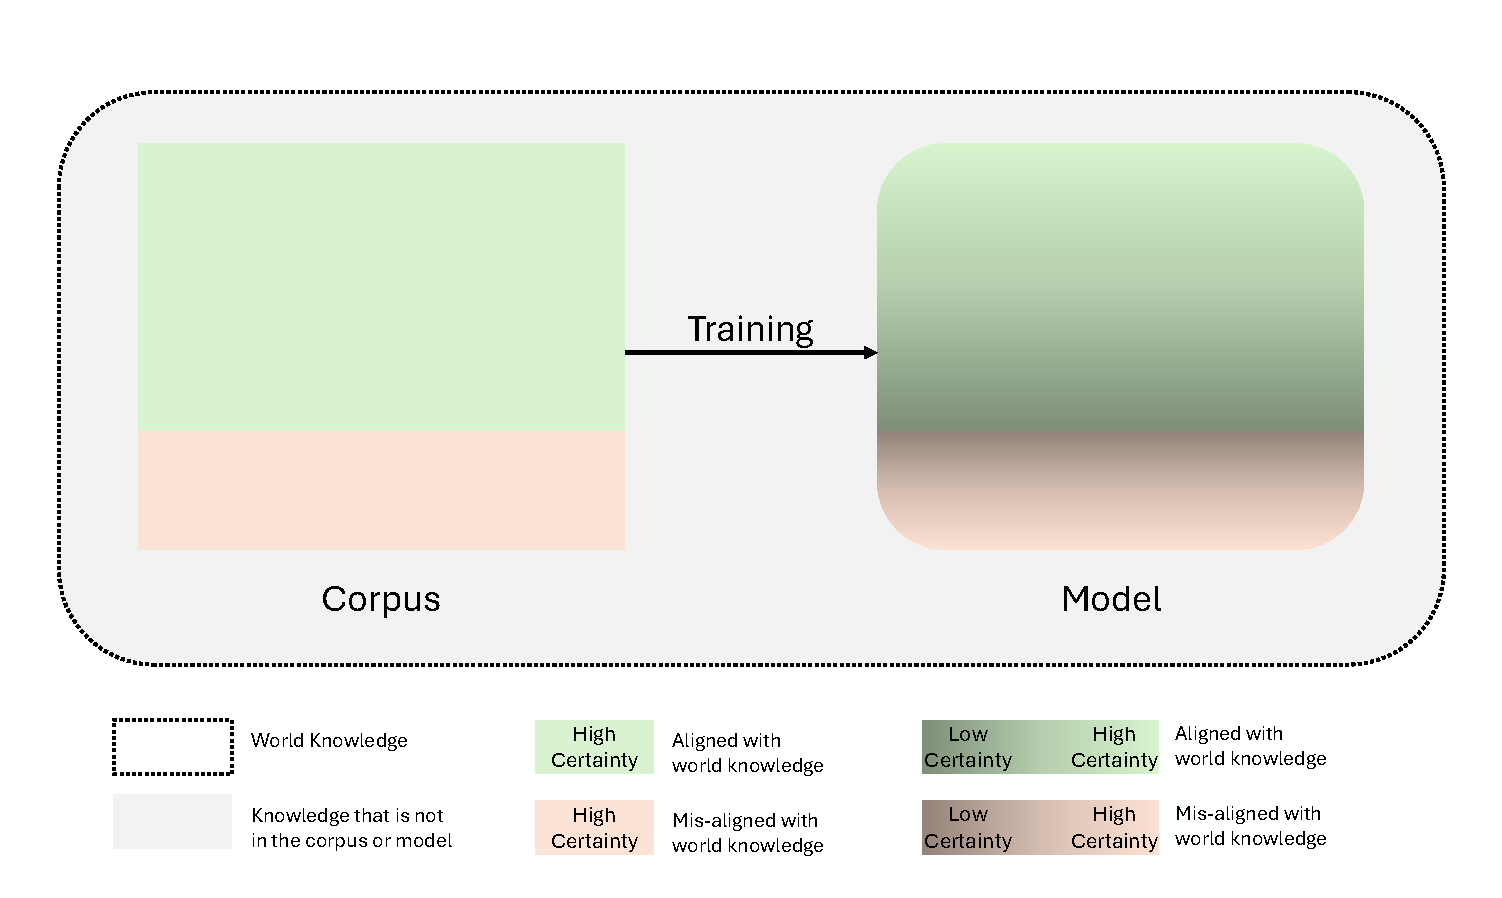
\includegraphics[width=\linewidth]{figures/knowledge.pdf}
    \caption{World Knowledge, Training Corpus and Language Model}
    \label{fig:knowledge}
\end{figure}

Therefore, we need to improve Internal Consistency and eliminate vagueness within the model to enhance its confidence in correct knowledge. However, eliminating vagueness also means that the model will be equally confident in erroneous knowledge. This raises a question: does enhancing consistency yield overall benefits or drawbacks? The advantage is that when preprocessing and cleaning the pre-training corpus, the intention is to align it towards world knowledge (correct knowledge). Hence, we propose the ``Consistency Is (Almost) Correctness'' hypothesis.

\begin{tcolorbox}[colback=white!98!black,colframe=white!30!black,boxsep=1.1pt,top=6.75pt]%
\vspace{1.75pt}%
\textbf{Consistency Is (Almost) Correctness}\\[-0.575em]
\noindent\makebox[\textwidth]{\rule{\textwidth}{0.4pt}}
\\[0.25em]
Enhancing a language model's internal consistency activates its cognitive certainty, reinforcing both correct and erroneous knowledge. However, because the pre-training corpus is predominantly aligned with correct world knowledge, improving consistency tends to amplify correct content more than incorrect content. Consequently, increased internal consistency generally results in improved overall correctness.
\end{tcolorbox}

However, why do some opposing voices believe that improving consistency cannot enhance the model's correctness? We believe this is closely related to the testing tasks. Many works refuting Self-Feedback use testing tasks that lie in the shaded areas of Fig.~\ref{fig:knowledge} (e.g., unstated puzzles not in the training corpus or questions unsolvable without external knowledge). Models struggle to effectively Self-Evaluate and Self-Update for tasks beyond their generalization capability.

In summary, within-distribution capabilities, the Self-Feedback framework can enhance model consistency by reinforcing the model's fit to corpus priors, thereby eliminating uncertainty and improving consistency. According to the ``Consistency Is (Almost) Correctness'' hypothesis, this leads to an overall improvement in the model's performance.


% \subsection{Practical Suggestions}
% TODO 低优先级


% 既然有许多的争议,为了帮助大家更好地认识哪些方向对解决哪些任务更有帮助,我们提出一个技术路线图供大家参考,如图~\ref{fig:tech_map}所示。

% \begin{figure}[]
%     \centering
%     \includegraphics[width=\linewidth]{figures/placeholder.png}
%     \caption{技术路线图}
%     \label{fig:tech_map}
% \end{figure}


\subsection{Appeals}


\noindent Currently, there are many chaos in this field: using similarly expressed names, proposing rare or unrealistic tasks, using different benchmarks for the same task, and comparing different baselines. In summary, without clear debate topics, many works contradict each other, resulting in confusing conflicts of views. To avoid these confusions, we propose several appeals.

\begin{itemize}
    \item \textbf{Naming.} When proposing new methods, ensure names are appropriate and avoid conflicts (e.g., Self-Improve~\cite{SelfImprove_23_EMNLP_Illinois}, Self-Improvement~\cite{SelfImprovement_24_arXiv_Tencent}). Additionally, when classifying one's work, consider the accuracy of the direction name. For instance, uncertainty estimation and confidence estimation have different directional indicators; the former leans towards mechanistic explanation, while the latter leans towards application.

    \item \textbf{Task Definition.} Some work has begun to notice that reasoning elevation and hallucination alleviation are similar tasks. For example,~\cite{MAF_23_EMNLP_UCSB, SelfBias_24_arXiv_UCSB} propose methods that focus on both tasks. We advocate for using Internal Consistency Mining to refer to these two tasks, ensuring terminological standardization.

    \item \textbf{Reasoning and Hallucination.} Regarding the use of these two terms, we suggest that when dealing with tasks like QA, we can say that a method may lack reasoning ability; whereas for open-ended generation tasks, we can use exhibit hallucination.
    
    \item \textbf{Selection of Baselines.} This paper summarizes some relatively fixed lines of work, suggesting that when selecting comparison baselines, first determine the sub-direction for your work and choose important work within that direction as comparison baselines. Comparing across different lines of work can lead to unfair comparisons due to significant methodological differences.

    \item \textbf{Experiment Settings.} Unrealistic experimental task settings will not advance scientific research. For instance, requiring pre-given golden label to make predictions does not fit real-world needs~\cite{TheoryNoReason_24_ICLR_Google}.

    \item \textbf{Prompt Engineering.} As mentioned in Section~\ref{sec:conflict}, many works exhibit a prompt tuning phenomenon, where adjusting the prompt can reverse experimental results. Therefore, we propose that prompt templates must be disclosed in the paper or source code and provide clear usage instructions; verify the robustness of prompts, such as using various templates for experiments; and verify the generality of prompts, such as using multiple different LLMs for experiments.
\end{itemize}


\section{Future Directions and Challenges} \label{sec:future}


\subsection{Textual Self-Awareness}


\noindent Human speech often lacks consistency and certainty in expressing viewpoints. However, we typically use phrases like ``I'm not sure, but I think'' or ``I believe there's an 80\% chance'' to hedge, demonstrating our good self-awareness. Yona et al.~\cite{ExpressUncertainty_24_arXiv_TAU} proved that current models still cannot verbally and faithfully express their uncertainty. Kapoor et al.~\cite{MustTaught_24_arXiv_NYU} found similar issues and showed through experiments that models can achieve good calibration only after fine-tuning. How to enable models to utilize the available Internal Consistency signal to help textually express their self-awareness is a promising direction~\cite{ExpressKnowledge_24_arXiv_FDU}.


\subsection{The Reasoning Paradox}

\noindent As mentioned in Section~\ref{sec:hourglass}, there is a paradox between the reasoning done during single token prediction (latent reasoning~\cite{TheoryLatentReason_24_arXiv_Google}) and the reasoning done using multiple tokens in language (explicit reasoning, e.g., CoT).

\begin{tcolorbox}[colback=white!98!black,colframe=white!30!black,boxsep=1.1pt,top=6.75pt]%
\vspace{1.75pt}%
\textbf{The Paradox of Latent and Explicit Reasoning}\\[-0.575em]
\noindent\makebox[\textwidth]{\rule{\textwidth}{0.4pt}}
\\[0.25em]
Language models excel in latent reasoning when decoding a single token, effectively utilizing attention mechanisms and deep feature interactions to achieve accurate reasoning. However, single tokens can't answer complex questions. Explicit reasoning, which involves generating a sequence of tokens (e.g. CoT), enhances the model's problem-solving capabilities. Yet, lengthy reasoning chains and inherent noise in text disrupt the model's latent reasoning. Thus, there is a paradox between latent reasoning and explicit reasoning.
\end{tcolorbox}
% TODO:可以考虑增加示意图

Therefore, we need to study the equilibrium point between latent and explicit reasoning, enabling efficient use of reasoning resources and improving the model's reasoning efficiency. Currently, there is little research on this issue.


\subsection{Dive Deeper}


\noindent From the seven lines of work we summarized, many works optimize only at the response layer. However, this approach relies on experience and is highly sensitive to prompt templates. Moreover, the low entry barrier and extensive participation in such work have led to an influx of low-quality papers. Therefore, we encourage researchers to delve into the decoding layer and latent layer, exploring more universal discoveries from an interpretability perspective.


\subsection{The Unified Perspective}


\noindent At present, the focus of work in this field is relatively narrow, lacking a comprehensive understanding of the entire field, and consequently, there are no more general framework works. We believe that using the perspective proposed in this paper, considering problems from the response, decoding, and latent layers in a unified manner, can better facilitate Internal Consistency Mining. There are emerging efforts that begin to integrate multiple layers. For example, Xie et al.~\cite{CalibIC_24_arXiv_SJTU} start from the response layer and reflects on how different CoT paths guide the consistency of the latent layer; Xie et al.~\cite{SelfEvaluation_23_NeuIPS_NUS} use Self-Evaluation strategies at the response layer to guide better decoding strategies.


\subsection{The Comprehensive Evaluation}


\noindent Different LLMs, combined with various Self-Feedback strategies, can produce vastly different combinations. However, as explained in Section~\ref{sec:evaluation}, current evaluation methods generally have a singular focus, making it difficult to comprehensively and conveniently understand the model's capabilities. Therefore, building a complete evaluation system from meta evaluation to common evaluation, from latent states to response, from benchmark to metric, and from uncertainty to feedback is a worthy consideration.


% TODO 暂不重要
% \subsection{Internal Consistency 建模}


\section{Limitations}


\noindent Given the terminological confusion and overlapping lines of work in this field, the sections of this paper are not necessarily orthogonal. Consequently, a single work may fall into multiple categories, indicating that the method employs ideas from different lines of work. The writing design is more inspirational, helping researchers to answer: What is the position of their work in a grand system? What are its advantages and disadvantages? What should be the next step in designing new and better methods?


\section{Conclusion}


\noindent This paper proposes using an Internal Consistency perspective to observe the most prominent phenomena in the field of LLMs: lack of reasoning and the presence of hallucinations. The article explains the modeling of Internal Consistency, the hourglass evolution pattern, the current status, sources, and significance from multiple aspects, and proposes the Self-Feedback framework for Internal Consistency Mining. We summarize the various tasks and distinctive lines of work involved in the Self-Feedback framework. These lines of work can help researchers locate their work's position within a vast system and facilitate reasonable experimental comparisons. Finally, we include three critical topics: relevant evaluation methods and benchmarks, exploring whether Self-Feedback truly works, and future research directions. In summary, this paper attempts to use a deeper research perspective (Internal Consistency) and a more general framework (Self-Feedback) to summarize a series of important works on reasoning elevation and hallucination alleviation.


\section*{Acknowledgments}

\noindent This work was supported by the National Natural Science Foundation of China (Grants No. 62072463, 71531012), the National Social Science Foundation of China (Grants No. 18ZDA309), the Research Seed Funds of the School of Interdisciplinary Studies at Renmin University of China, and the Opening Project of the State Key Laboratory of Digital Publishing Technology of the Founder Group.



{\appendices
\section{Notations} \label{apdx:notation}

\begin{table}[h!]
\caption{Common Notations} \label{tab:symbols}
\centering
\begin{tabular}{p{1.2cm}p{6.5cm}}
\toprule
Symbol & Description \\ 
\midrule
$\boldsymbol{x}$ & Query \\ 
$\mathcal{M}, \mathcal{N}$ & LLMs \\ 
$e$ & Expression type, $e \in \{\text{response}, \text{decoding},\text{latent}\}$ \\
$O_e(\mathcal{M}, \boldsymbol{x})$ & Sampling distribution \\
$\mathcal{Y}$ & Sampling set \\ 
$\boldsymbol{y}_i$ & The $i$-th element in the sampling set \\ 
$\boldsymbol{y}_{0:i}$ & Elements from $0$ to $i$ in the sampling set \\ 
$y^t$ & The $t$-th token in text $\boldsymbol{y}$ \\ 
$f$ & Consistency Signal of Self-Feedback \\ 
$P(\boldsymbol{y}|\boldsymbol{x};\theta)$ & Probability that model parameterized by $\theta$ outputs $\boldsymbol{y}$ given input $\boldsymbol{x}$ \\ 
\bottomrule
\end{tabular}
\end{table}

\section{The Five Responses of GPT-4o} \label{apdx:GPT4o}

\noindent Fig.~\ref{fig:response1_from_gpt4o}, ~\ref{fig:response2_from_gpt4o}, ~\ref{fig:response3_from_gpt4o}, ~\ref{fig:response4_from_gpt4o}, and~\ref{fig:response5_from_gpt4o} show five different responses obtained when querying GPT-4o: How many full stops (periods) are there: ``.!..!..!''. The experiments were conducted on June 14, 2024, accessed via the official website\footnote{\url{https://chat.openai.com/}}.

\begin{figure}[h!]
\small
\centering
\begin{tcolorbox}[colback=blue!5!white,colframe=blue!75!black,title=GPT-4o Response 1,fontupper=\footnotesize,fonttitle=\scriptsize]
To determine the number of full stops (periods) in the string ".!..!..!", we need to count the occurrences of the character '.'. \\
Let's break down the string: \\
1. ".!": 1 full stop \\
2. "..!": 2 full stops \\
3. ".!": 1 full stop \\
Summing these up: \\
1 + 2 + 1 = 4 \\
Therefore, there are 4 full stops in the string ".!..!..!".
\end{tcolorbox}
\caption{GPT-4o Response 1}
\label{fig:response1_from_gpt4o}
\end{figure}

\begin{figure}[h!]
\small
\centering
\begin{tcolorbox}[colback=blue!5!white,colframe=blue!75!black,title=GPT-4o Response 2,fontupper=\footnotesize,fonttitle=\scriptsize]
The sequence ".!..!..!" contains three instances of "." (full stops or periods). Each segment ".!" has one full stop, and there are three such segments.
\end{tcolorbox}
\caption{GPT-4o Response 2}
\label{fig:response2_from_gpt4o}
\end{figure}

\begin{figure}[h!]
\small
\centering
\begin{tcolorbox}[colback=blue!5!white,colframe=blue!75!black,title=GPT-4o Response 3,fontupper=\footnotesize,fonttitle=\scriptsize]
The string ".!..!..!" contains a total of **3** full stops (periods).
\end{tcolorbox}
\caption{GPT-4o Response 3}
\label{fig:response3_from_gpt4o}
\end{figure}



\begin{figure}[h!]
\small
\centering
\begin{tcolorbox}[colback=blue!5!white,colframe=blue!75!black,title=GPT-4o Response 4,fontupper=\footnotesize,fonttitle=\scriptsize]
The string ".!..!..!" contains full stops (periods). To determine the number of full stops in this string, we simply count the occurrences of the period character ('.'). Let's analyze the string: \\
- The first character is a period. \\
- The second character is an exclamation mark. \\
- The third character is a period. \\
- The fourth character is an exclamation mark. \\
- The fifth character is a period. \\
- The sixth character is an exclamation mark. \\
- The seventh character is a period. \\
- The eighth character is an exclamation mark. \\
Counting the periods: \\
1. The first period is at position 1. \\
2. The second period is at position 3. \\
3. The third period is at position 5. \\
4. The fourth period is at position 7. \\
Therefore, there are 4 full stops (periods) in the string ".!..!..!".
\end{tcolorbox}
\caption{GPT-4o Response 4}
\label{fig:response4_from_gpt4o}
\end{figure}



\begin{figure}[h!]
\small
\centering
\begin{tcolorbox}[colback=blue!5!white,colframe=blue!75!black,title=GPT-4o Response 5,fontupper=\footnotesize,fonttitle=\scriptsize]
The sequence ".!..!..!" contains the following characters: \\
1. Period (.) \\
2. Exclamation mark (!) \\
3. Period (.) \\
4. Exclamation mark (!) \\
5. Period (.) \\
6. Exclamation mark (!) \\
To count the full stops (periods): \\
1. The first character is a period. \\
2. The third character is a period. \\
3. The fifth character is a period. \\
There are a total of **three** periods in the sequence ".!..!..!".
\end{tcolorbox}
\caption{GPT-4o Response 5}
\label{fig:response5_from_gpt4o}
\end{figure}


\section{Experiment Details of Three Types of Consistency} \label{apdx:experiment}


\noindent The setups and results of the comparative experiments on three different types of consistency are shown in Tables~\ref{tab:apdxtab1}, ~\ref{tab:apdxtab2}, and ~\ref{tab:apdxtab3}. Here, Fix $\text{attn}^{16}_{15}$ refers to keeping the 16th attention head in the 15th layer unchanged, while zero out $\text{attn}^{i \neq 16}_{15}$ denotes zeroing out all attention heads in the 15th layer except the 16th one. The source code for this experiment is available in our open-source GitHub repository.


\begin{table}[h!]
\centering
\caption{Latent Consistency}\label{tab:apdxtab1}
\begin{tabular}{lc}
\toprule
Setting                                                                 & Selected Token \\
\midrule
Fix $\text{attn}^0_0$; Zero out $\text{attn}^{i \neq 0}_0$              & 0              \\
Fix $\text{attn}^{16}_0$; Zero out $\text{attn}^{i \neq 16}_0$          & 0              \\
Fix $\text{attn}^0_{15}$; Zero out $\text{attn}^{i \neq 0}_{15}$        & 5              \\
Fix $\text{attn}^{16}_{15}$; Zero out $\text{attn}^{i \neq 16}_{15}$    & 4              \\
Fix $\text{attn}^0_{30}$; Zero out $\text{attn}^{i \neq 0}_{30}$        & 4              \\
Fix $\text{attn}^{16}_{30}$; Zero out $\text{attn}^{i \neq 16}_{30}$    & 4              \\
\bottomrule
\end{tabular}
\end{table}

\begin{table}[h!]
\centering
\caption{Decoding Consistency}\label{tab:apdxtab2}
\begin{tabular}{lc}
\toprule
Decoding Strategy                      & Selected Token \\
\midrule
Greedy Decoding                        & 4              \\
Beam Search Decoding ($\text{beam}=5$) & 4              \\
Sampling Decoding                      & 3              \\
Top-k Sampling Decoding ($k=50$)       & 4              \\
Top-p Sampling Decoding ($p=0.95$)     & 4              \\
\bottomrule
\end{tabular}
\end{table}


\begin{table}[h!]
\centering
\caption{Response Consistency}\label{tab:apdxtab3}
\begin{tabular}{p{0.95\linewidth}}
\toprule
Model Response                                                                                                                                                     \\
\midrule
\textbf{RESPONSE 1}: There is a period after the first dot, then another period after the second dot, and so on. So, there are 5 periods in total.                                      \\
\textbf{RESPONSE 2}: There is one full stop after the first "!", then another after the second "!", and another after the third "!". So, there are 3 full stops in total.               \\
\textbf{RESPONSE 3}: There is one full stop after the first "!", then another after the second "!", and so on. So, there are 3 full stops.                                              \\
\textbf{RESPONSE 4}: There is one period at the end of the first part, then another after the second part, and finally one more after the third part. So, there are 3 periods in total. \\
\textbf{RESPONSE 5}: There is 1 period, then another one, and another one... So, there are 3 full stops!                                                                               \\
\bottomrule
\end{tabular}
\end{table}


% \section{文献计量分析}
% TODO 未来可以考虑

% 重要学者:Liangming Pan,Mor Geva

% xxx xxx xxx xxx xxx xxx xxx xxx xxx xxx xxx xxx xxx xxx xxx xxx xxx xxx xxx xxx xxx xxx xxx xxx xxx xxx xxx xxx 
}

% \clearpage

% \balance
\bibliographystyle{IEEEtran}
\bibliography{IEEEabrv,references}


\begin{IEEEbiography}[{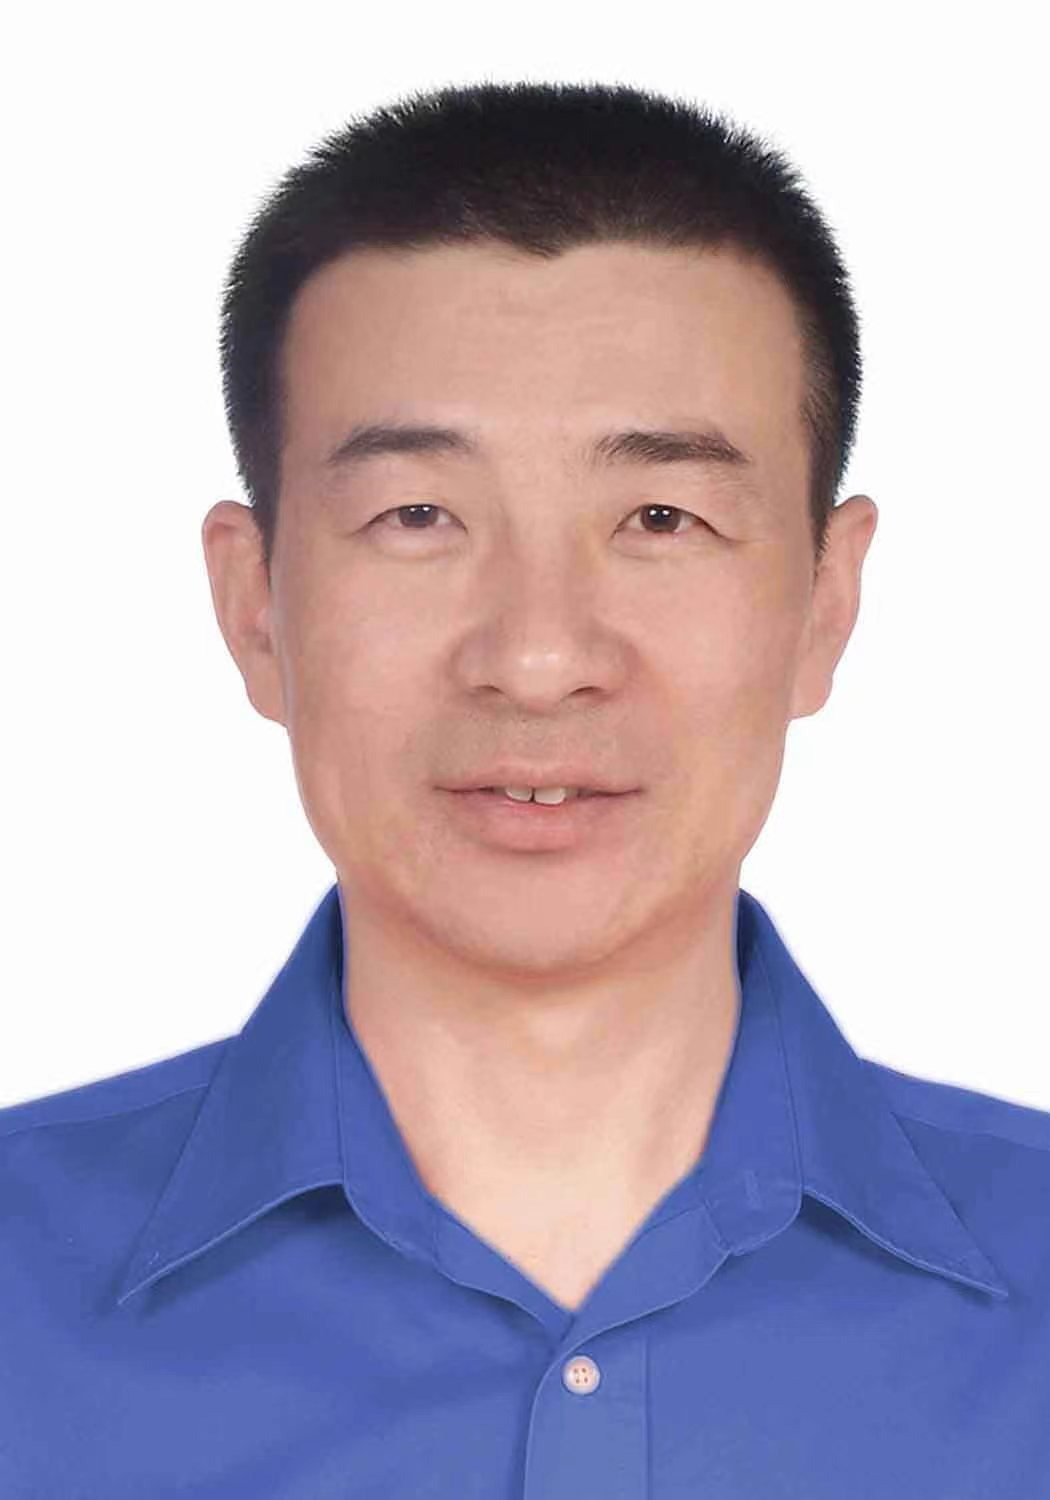
\includegraphics[width=1in,height=1.25in,clip,keepaspectratio]{photos/lx.jpg}}]{Xun Liang}
(Senior Member, IEEE) received the B.Sc. and Ph.D. degrees in computer engineering from Tsinghua University, Beijing, China, in 1989 and 1993, respectively, and the M.Sc. degree in operations research from Stanford University, Palo Alto, CA, USA, in 1999. He worked as a Post-Doctoral Fellow with the Institute of Computer Science and Technology, Peking University, Beijing, from 1993 to 1995, and with the Department of Computer Engineering, University of New Brunswick, Fredericton, NB, Canada, from 1995 to 1997. He worked as a CTO, leading over ten intelligent information products in RixoInfo Ltd., CA, USA, from 2000 to 2007, and was the Director of the Data Mining Lab, Institute of Computer Science and Technology, Peking University, from 2005 to 2009. He is currently a professor with the School of Information, Renmin University of China. His research interests include support vector machines, social computing and large language models.
\end{IEEEbiography}

\vskip -2\baselineskip plus -1fil

\begin{IEEEbiography}[{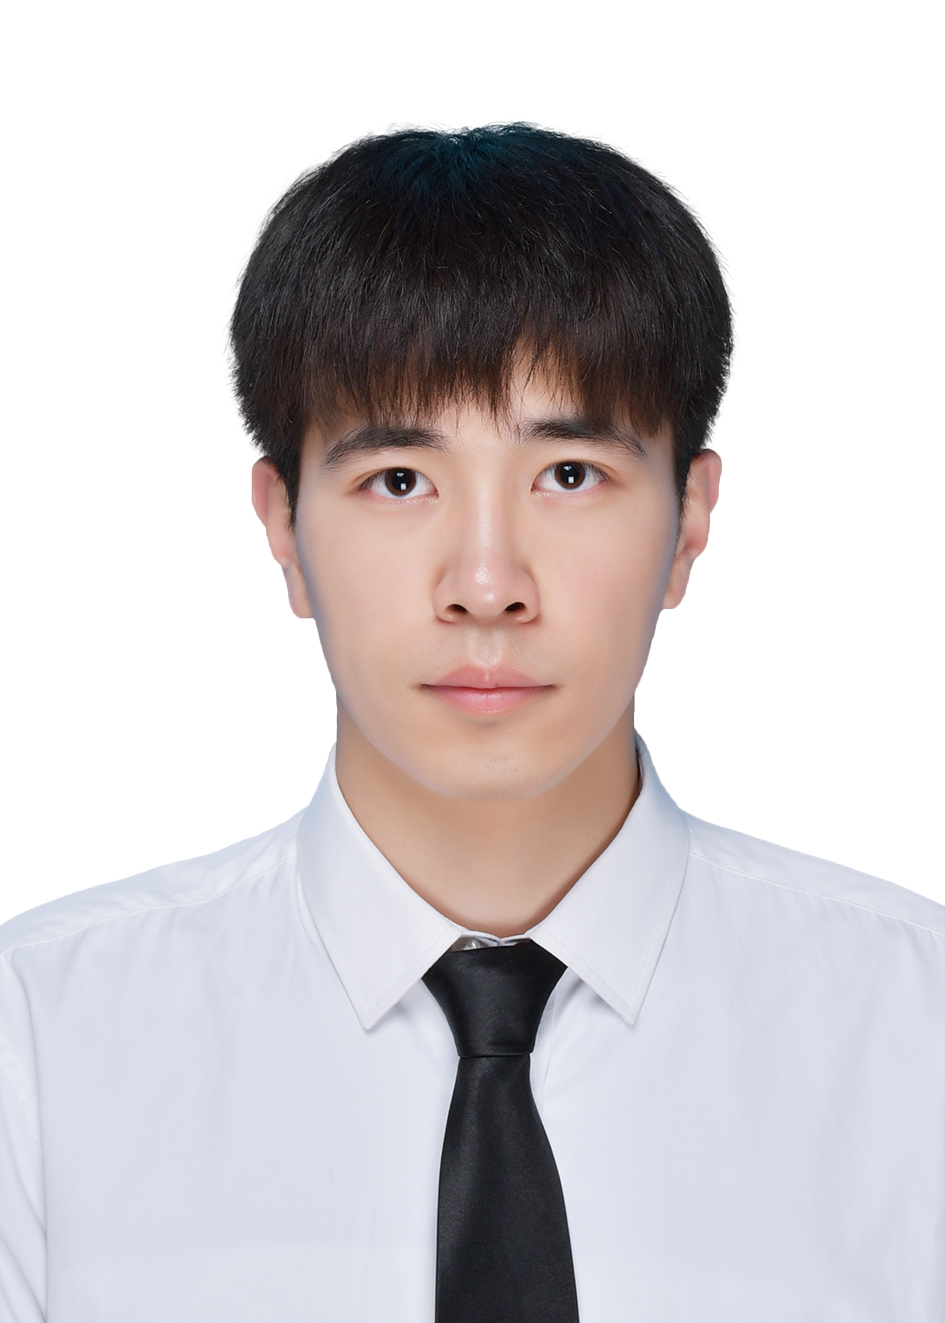
\includegraphics[width=1in,height=1.25in,clip,keepaspectratio]{photos/ssc.jpg}}]{Shichao Song}
is currently a PhD student at the School of Information, Renmin University of China, under the supervision of Prof. Xun Liang. His research interests span a wide range of topics, including internal consistency mining of LLMs, LLM interpretability, and reliable evaluation methods for LLMs. For more information, visit his website at \url{https://ki-seki.github.io/}.
\end{IEEEbiography}

\vskip -2\baselineskip plus -1fil

\begin{IEEEbiography}[{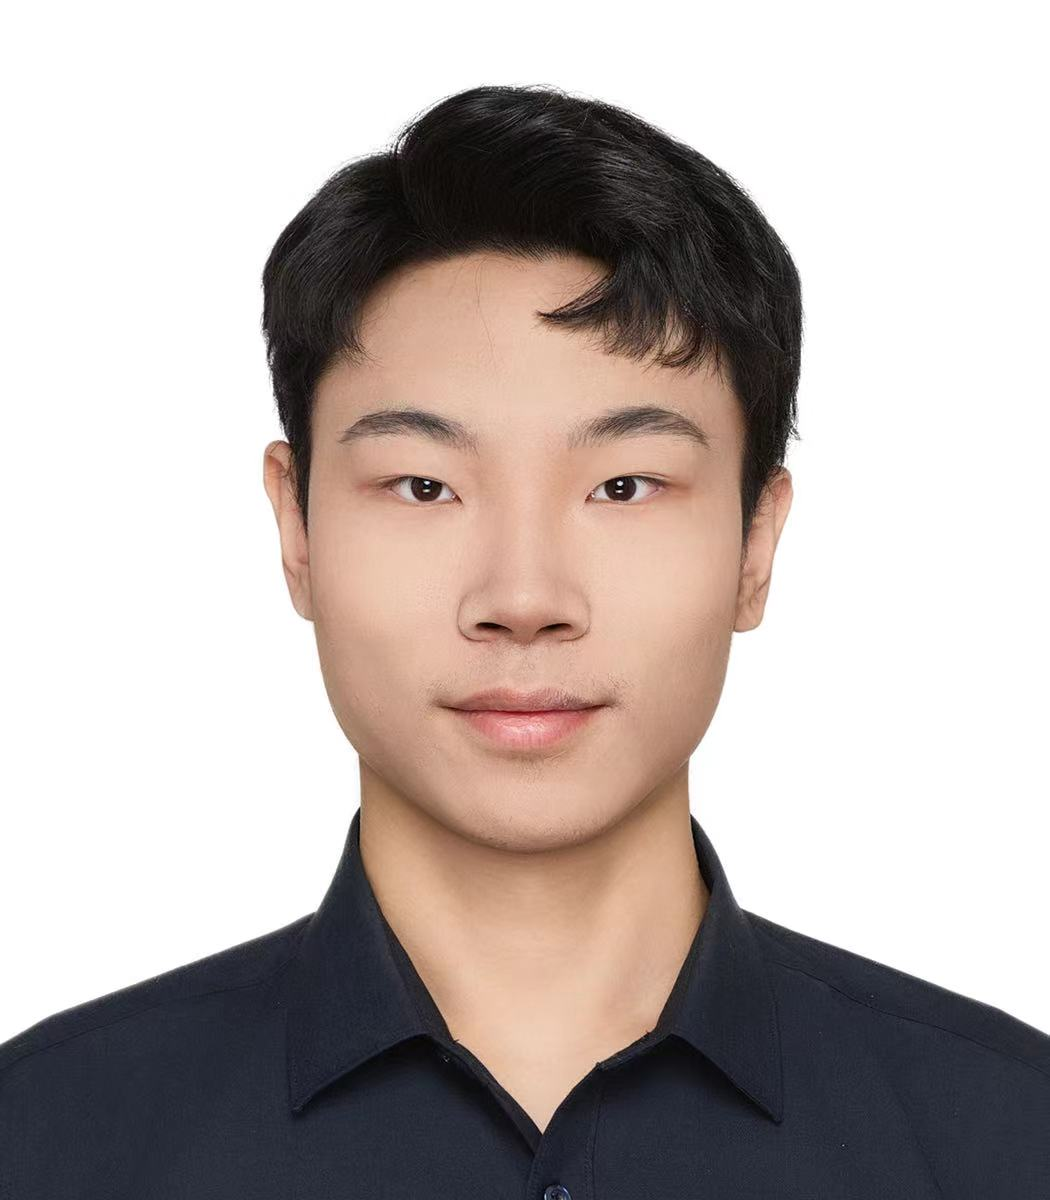
\includegraphics[width=1in,height=1.25in,clip,keepaspectratio]{photos/zzf.jpg}}]{Zifan Zheng}
is currently a research intern at the Large Language Model Center of the Institute for Advanced Algorithms Research, Shanghai. He received the B.S. degree in Computer Science and Technology from Beijing Institute of Technology, China, in 2024. His research interests include LLMs interpretability, reliable evaluation and social network analysis.
\end{IEEEbiography}

\vskip -2\baselineskip plus -1fil

\begin{IEEEbiography}[{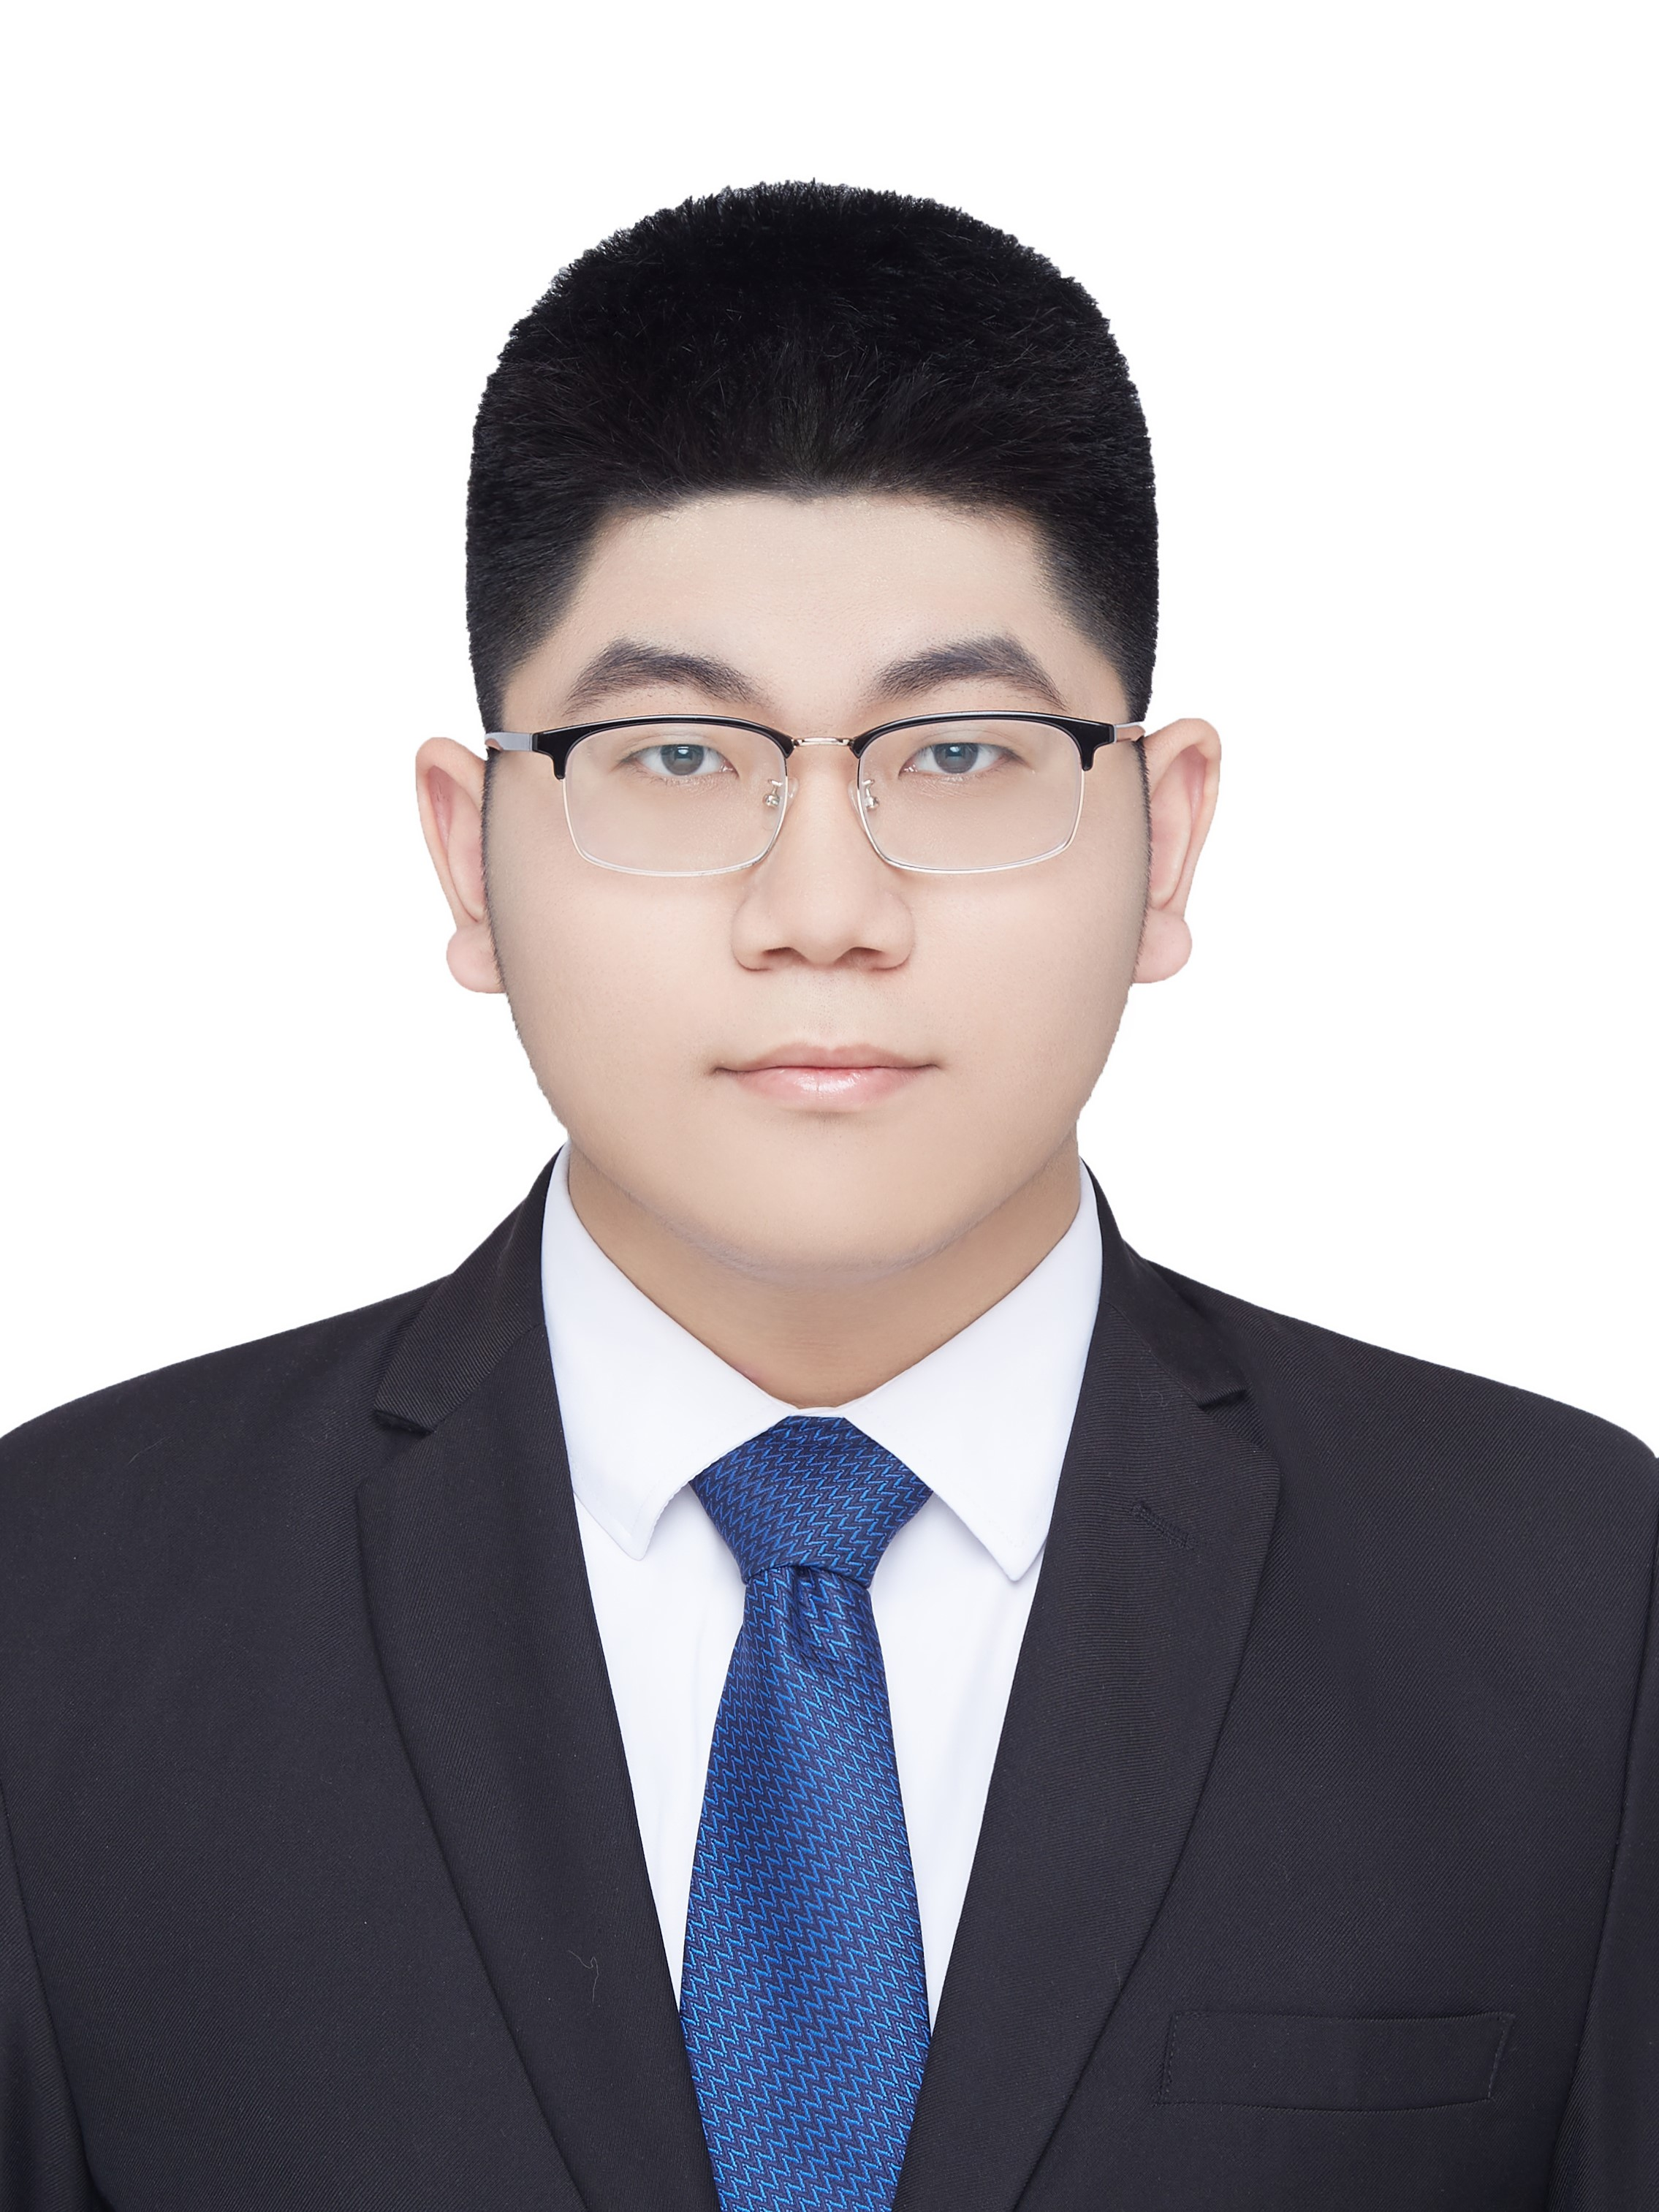
\includegraphics[width=1in,height=1.25in,clip,keepaspectratio]{photos/why.jpg}}]{Hanyu Wang}
is a Ph.D. student at the School of Information, Renmin University of China, under the supervision of Professor Xun Liang. His research areas include large language models, controllable text generation in large language models, and controlled decoding.
\end{IEEEbiography}

\vskip -2\baselineskip plus -1fil

\begin{IEEEbiography}[{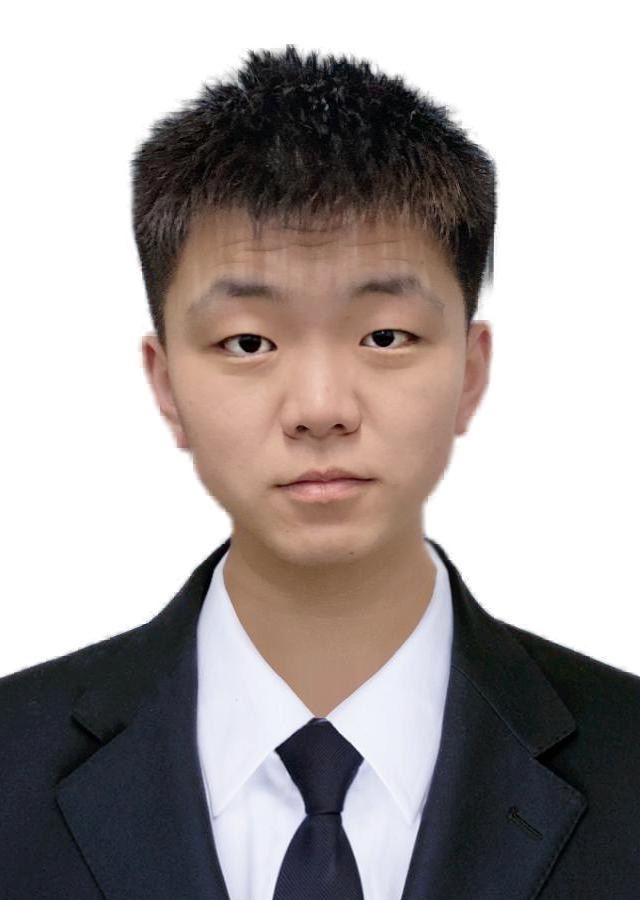
\includegraphics[width=1in,height=1.25in,clip,keepaspectratio]{photos/yqc.jpg}}]{Qingchen Yu}
is currently a research intern at the Large Language Model Center of the Institute for Advanced Algorithms Research in Shanghai. He is also a master's student at Shanghai University. His research interests include machine learning, LLM evaluation, and prompt engineering.
\end{IEEEbiography}

\vskip -2\baselineskip plus -1fil

\begin{IEEEbiography}[{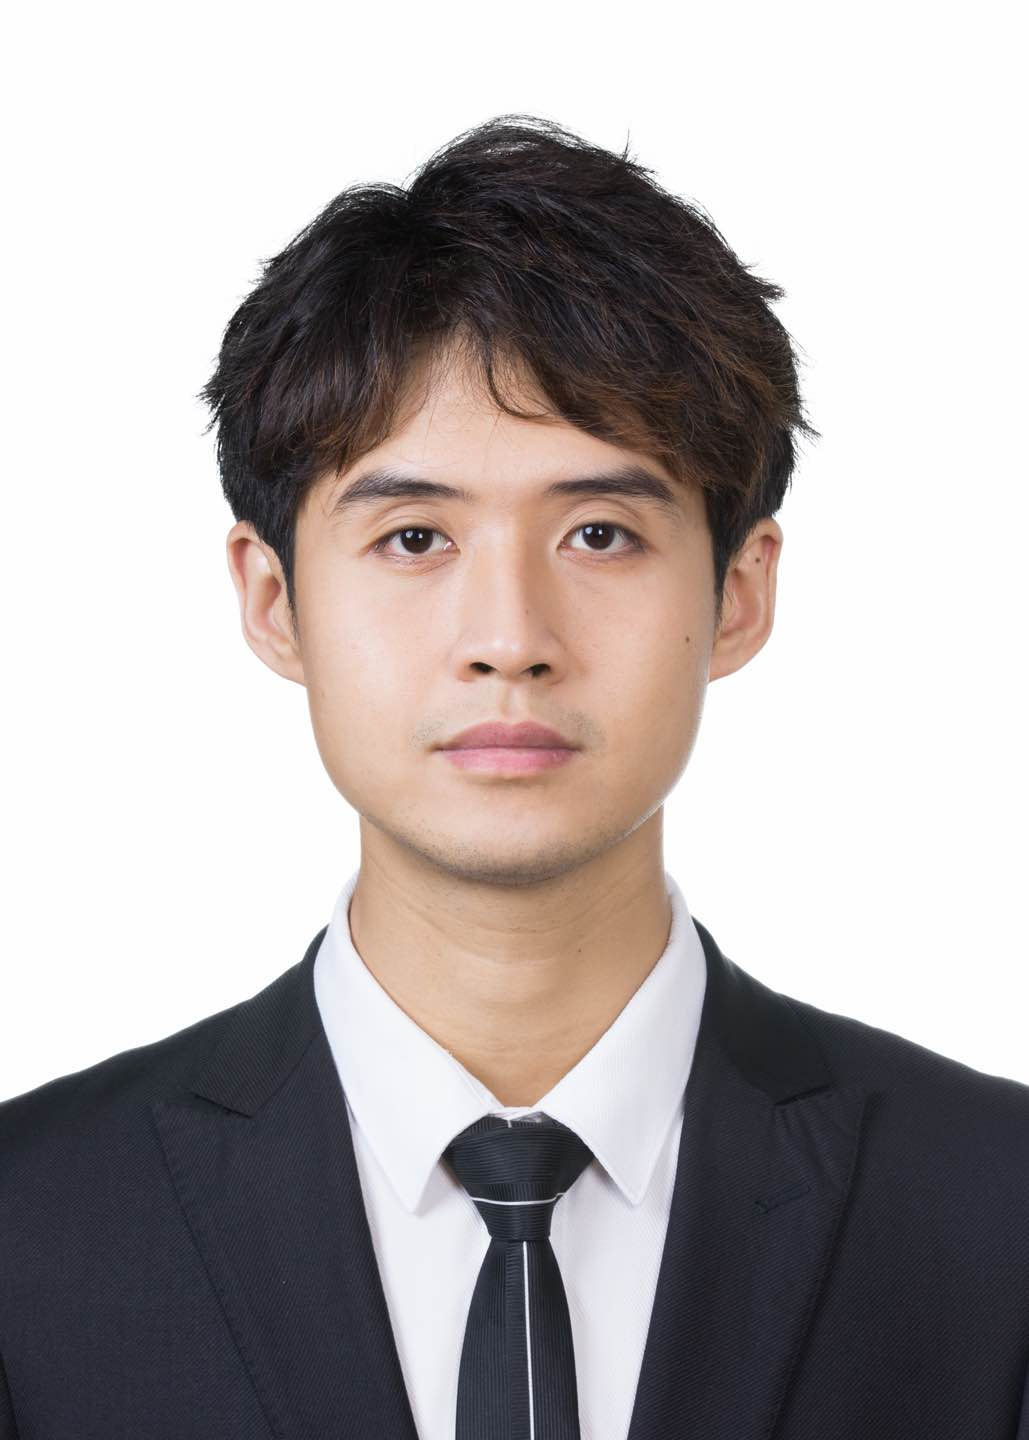
\includegraphics[width=1in,height=1.25in,clip,keepaspectratio]{photos/lxk.jpeg}}]{Xunkai Li} is currently working toward the PhD degree with the school of Computer Science, Beijing Institute of Technology, advised by Prof. Rong-Hua Li. He received the BS degree in computer science from Shandong University in 2022. His research interest lies in Data-centric ML and Graph-ML within complex relational data and new learning paradigms. He has published 5+ papers in top DB/DM/AI conferences such as VLDB, WWW, AAAI as the first author.
\end{IEEEbiography}

 \vskip -2\baselineskip plus -1fil
 
\begin{IEEEbiography}[{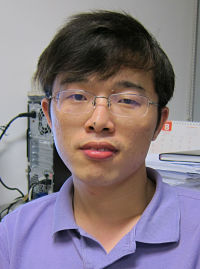
\includegraphics[width=1in,height=1.25in,clip,keepaspectratio]{photos/lrh.jpg}}]{Rong-Hua Li} received the Ph.D. degree in computer science from The Chinese University of Hong Kong, Hong Kong, in 2013. He is currently a Professor with the Beijing Institute of Technology, Beijing, China. His research interests include graph data management and mining, social network analysis, graph computation systems, and graph-based machine learning.
\end{IEEEbiography}

\vskip -2\baselineskip plus -1fil

\begin{IEEEbiography}[{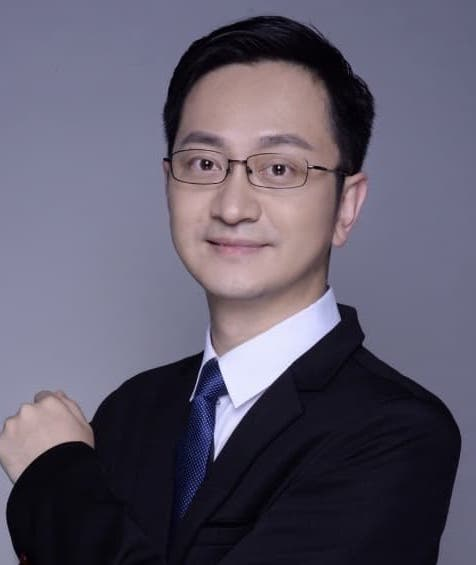
\includegraphics[width=1in,height=1.25in,clip,keepaspectratio]{photos/xfy.jpg}}]{Feiyu Xiong} is the Head of the Large Language Model Center of the Institute for Advanced Algorithms Research-Shanghai. He holds a Bachelor's degree from Huazhong University of Science and Technology and a Ph.D. from Drexel University. He has previously served as the Head of Data Intelligence for Alibaba's Business Middle Platform and the Head of the Data Platform for Taobao and Tmall Group. During his tenure at Alibaba, he was primarily responsible for the intelligent construction of systems related to core e-commerce transactions.
\end{IEEEbiography}

\vskip -2\baselineskip plus -1fil

\begin{IEEEbiography}[{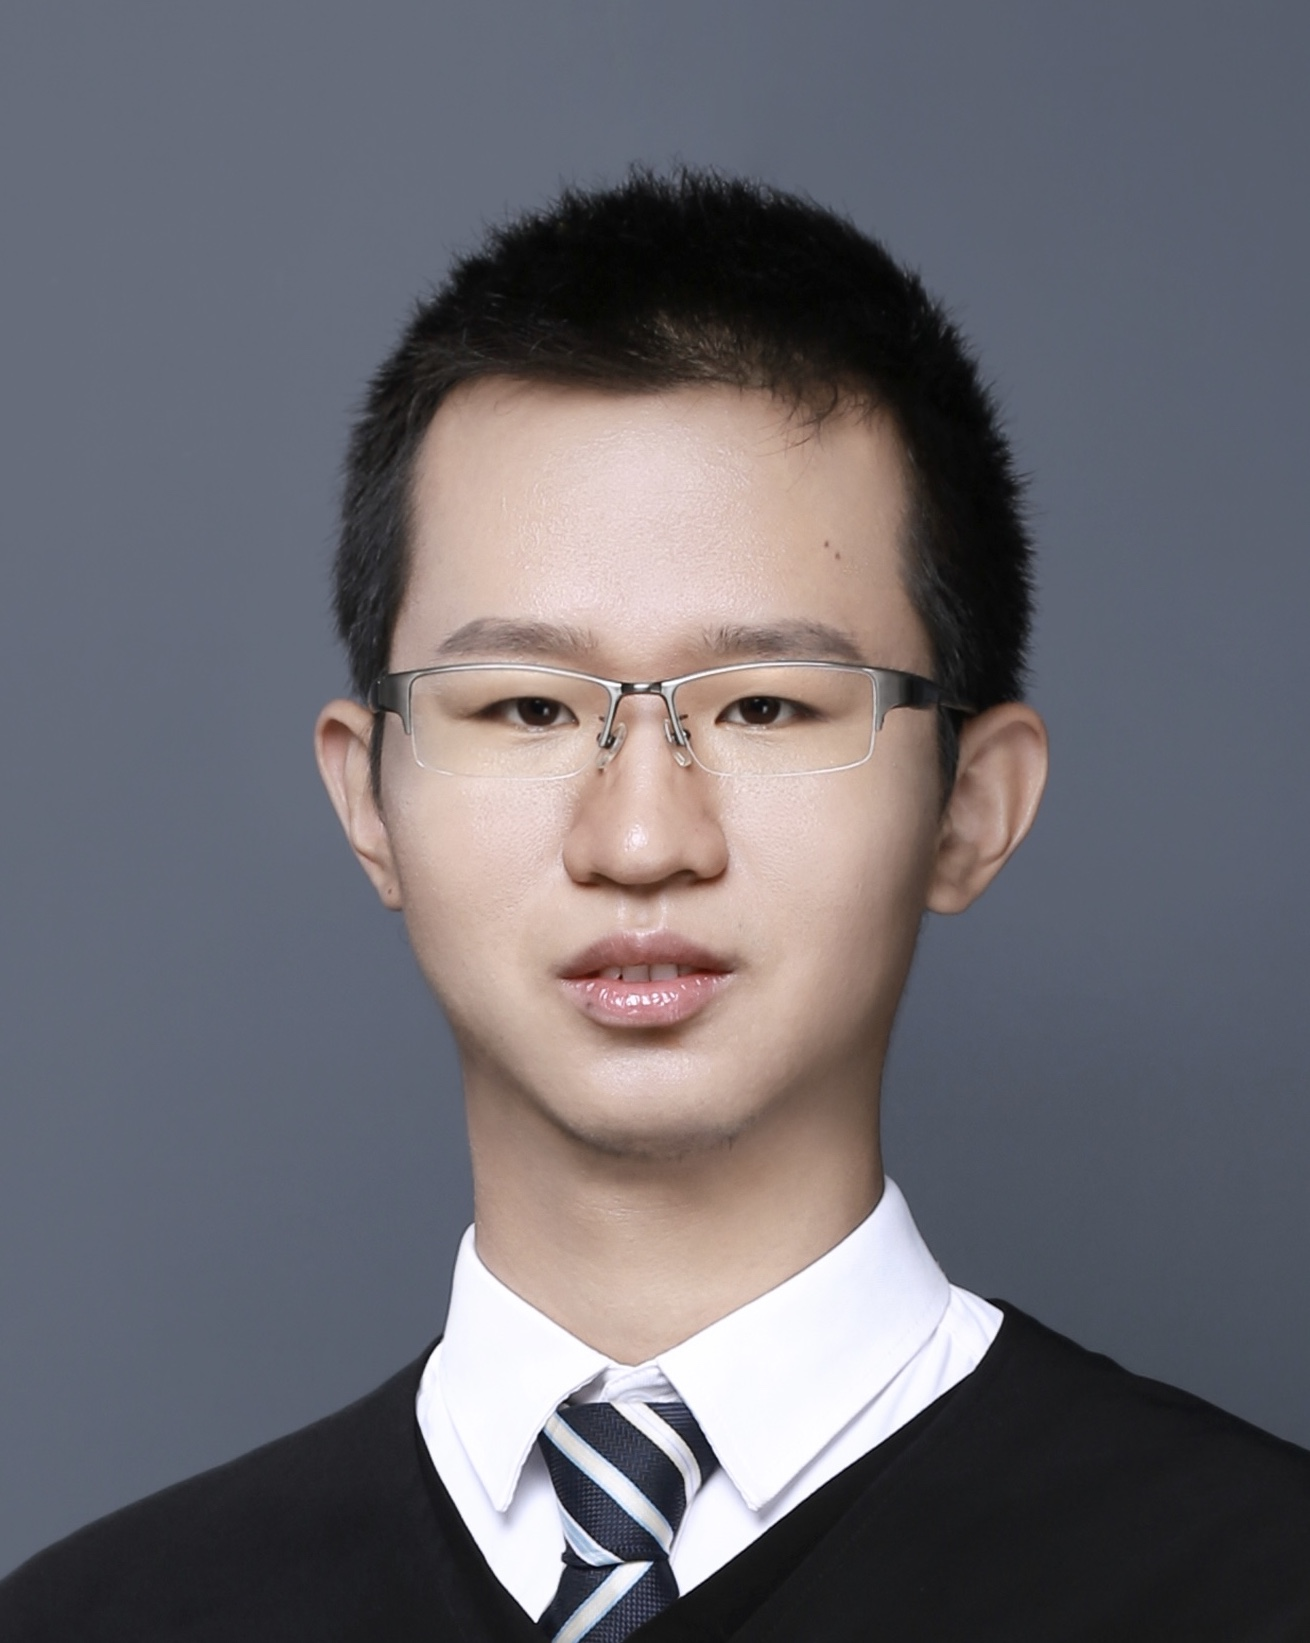
\includegraphics[width=1in,height=1.25in,clip,keepaspectratio]{photos/lzy.jpg}}]{Zhiyu Li} received his Ph.D. in Computer Science from the School of Information, Renmin University of China, in 2019. He is currently a Senior Researcher at the Large Language Model Center of the Institute for Advanced Algorithms Research-Shanghai. He has published over 30 papers in top-tier conferences and journals such as TKDE, KDD, and ACL. His current responsibilities include research and application implementation related to large language models. His research interests include model pre-training, model alignment, and hallucination optimization.
\end{IEEEbiography}

\vfill % This command ends the paragraph at the spot and adds the filling vertical space.


\end{document}
